\documentclass{../../common/projectreport}
\newcommand{\norm}[3]{{\left\|#1\right\|}_{#2}^{#3}}
\newcommand{\normball}[2]{{\mathbb{B}_{#1}^{#2}}}
\newcommand{\proximal}[2]{{\prox_{#1}(#2)}}
\newcommand{\forAll}{{\forall \,}}
\newcommand{\Rbb}{{\mathbb R}}
\newcommand{\Rbf}{{\mathbf R}}
\newcommand{\Lhat}{{\hat{L}}}
\newcommand{\Shat}{{\hat{S}}}
\newcommand{\Yhat}{{\hat{Y}}}
\newcommand{\Xhat}{{\hat{X}}}
\newcommand{\Nbb}{{\mathbb N}}
\newcommand{\Fbb}{{\mathbb F}}
\newcommand{\Cbb}{{\mathbb C}}
\newcommand{\Tbb}{{\mathbb T}}
\newcommand{\Zbb}{{\mathbb Z}}
\newcommand{\etabar}{{\bar{\eta}}}
\newcommand{\kbar}{{\bar{k}}}
\newcommand{\rbar}{{\bar{r}}}
\newcommand{\xibar}{{\bar{\xi}}}
\newcommand{\ubar}{{\bar{u}}}
\newcommand{\vbar}{{\bar{v}}}
\newcommand{\uhat}{{\hat{u}}}
\newcommand{\vbf}{{\mathbf{v}}}
\newcommand{\vhat}{{\hat{v}}}
\newcommand{\xbar}{{\bar{x}}}
\newcommand{\xhat}{{\hat{x}}}
\newcommand{\xdot}{{\dot{x}}}
\newcommand{\Xdot}{{\dot{X}}}
\newcommand{\xtilde}{{\tilde{x}}}
\newcommand{\xtildedot}{{\dot{\tilde{x}}}}
\newcommand{\Phitilde}{{\tilde{\Phi}}}
\newcommand{\phat}{{\hat{p}}}
\newcommand{\shat}{{\hat{s}}}
\newcommand{\xbf}{{\mathbf{x}}}
\newcommand{\wbf}{{\mathbf{w}}}
\newcommand{\Pbf}{{\mathbf{P}}}
\newcommand{\Xbf}{{\mathbf{X}}}
\newcommand{\Ebf}{{\mathbf{E}}}
\newcommand{\Obf}{{\mathbf{0}}}
\newcommand{\ebf}{{\mathbf{e}}}
\newcommand{\alphabf}{{\mathbf{\alpha}}} 
\newcommand{\alphabar}{{\bar{\alpha}}} 
\newcommand{\sgn}{\text{sgn}}
\newcommand{\Range}{\mathcal{R}}
\newcommand{\Nullspace}{\mathcal{N}}

\newcommand{\pderiv}[2]{\frac{\partial #1}{\partial #2}}
\newcommand{\pderivsq}[2]{\frac{\partial^2 #1}{\partial #2^2}}
\newcommand{\pderivxy}[3]{\frac{\partial^2 #1}{\partial #2 \partial #3}}

\newcommand{\One}{{\mathbf{1}}}

\newcommand{\Ccal}{{\mathcal{C}}}
\newcommand{\Dcal}{{\mathcal{D}}}
\newcommand{\Fcal}{{\mathcal{F}}}
\newcommand{\Hcal}{{\mathcal{H}}}
\newcommand{\Lcal}{{\mathcal{L}}}
\newcommand{\Ncal}{{\mathcal{N}}}
\newcommand{\Pcal}{{\mathcal{P}}}
\newcommand{\Qcal}{{\mathcal{Q}}}
\newcommand{\Rcal}{{\mathcal{R}}}
\newcommand{\Scal}{{\mathcal{S}}}
\newcommand{\Tcal}{{\mathcal{T}}}
\newcommand{\Ucal}{{\mathcal{U}}}
\newcommand{\Xcal}{{\mathcal{X}}}
\newcommand{\Ycal}{{\mathcal{Y}}}


\newcommand{\ifthen}[2]{\textbf{if} #1 \textbf{then} #2}
\newcommand{\ifthenreturn}[2]{\textbf{if} #1 \textbf{then return} #2}
\newcommand{\then}[1]{\textbf{then} #1}
\newcommand{\return}[1]{\textbf{return} #1}
\newcommand{\returns}[1]{\textbf{returns} #1}
\newcommand{\thenreturn}[1]{\textbf{then return} #1}
\newcommand{\foreachindo}[3]{\textbf{for each} #1 \textbf{in} #2 \textbf{do} #3}
\newcommand{\algindent}[1]{\STATE\hspace{#1\algorithmicindent}}

\DeclareMathOperator{\blkdiag}{blkdiag}
\DeclareMathOperator{\trace}{\mathbf{Tr}}
\DeclareMathOperator{\Convh}{Conv}
\DeclareMathOperator{\rank}{rk}
\DeclareMathOperator{\diag}{diag}
\DeclareMathOperator{\Realpart}{Re}
\DeclareMathOperator{\Imagpart}{Im}
\DeclareMathOperator{\Poles}{Poles}
\DeclareMathOperator{\spanspace}{span}
\DeclareMathOperator*{\argmax}{arg\,max}
\DeclareMathOperator*{\argmin}{arg\,min}
\DeclareMathOperator{\Onebf}{{\mathbf{1}}}
\DeclareMathOperator{\dom}{dom}
\DeclareMathOperator{\grad}{\nabla\!\!}
\DeclareMathOperator{\epi}{epi}
\DeclareMathOperator{\sign}{sign}
\DeclareMathOperator{\divergence}{div}
\DeclareMathOperator{\prox}{prox}

\newcommand\independent{\protect\mathpalette{\protect\independenT}{\perp}}
\def\independenT#1#2{\mathrel{\rlap{$#1#2$}\mkern2mu{#1#2}}}


\newcommand{\Acal}{{\mathcal{A}}}
\newcommand{\Abar}{{\bar{A}}}


\theoremstyle{plain}
\newtheorem{thm}{Theorem}
\theoremstyle{plain}
\newtheorem{fact}[thm]{Fact}
\theoremstyle{plain}
\newtheorem{prop}[thm]{Proposition}



%============================================================================================

\title{\Large EE227 Project Report \\ Robust Principal Component Analysis}
\author{Maximilian Balandat \and Walid Krichene \and Chi Pang Lam \and Ka Kit Lam}

%============================================================================================
\begin{document}
\maketitle

%============================================================================================
\section*{Introduction}
%TODO: general introduction goes here


%============================================================================================
%============================================================================================
\chapter{Theory}


\section{Introduction}
Given an observed matrix $M \in \Rbb^{n_1 \times n_2}$ that is formed as a superposition of a low-rank matrix $L_0$ and a sparse matrix $S_0$,
\[
M = L_0 + S_0
\]
Robust Principal Component Analysis \cite{Candes:2011fk} is the problem of recovering the low-rank and sparse components. Under suitable assumptions on the rank and incoherence of $L_0$, and the distribution of the support of $S_0$, the components can be recovered exactly with high probability, by solving the Principal Component Pursuit (PCP) problem given by

\begin{equation}
\begin{aligned}
&\text{minimize} && \|L\|_* + \lambda \|S\|_1 \\
&\text{subject to} && L+S = M
\label{eq:pcp}
\end{aligned}
\end{equation}

Principal component pursuit minimizes a linear combination of the nuclear norm of a matrix $L$ and the $\ell_1$ norm of $M-L$. Minimizing the $\ell_1$ norm is known to favor sparsity, while minimizing the nuclear norm $\|L\|_* = \sum_{\sigma \in \sigma(L)} \sigma$ is known to favour low-rank matrices (intuitively, favors sparsity of the vector of singular values).

The low-rank component $S_0$ is viewed as a noise matrix, that can represent measurement noise, failure in some sensors that will result in completely corrupting a fraction of the observed entries, or missing data (which translates to having a fraction of the entries equal to zero). In this setting, one would like to be able to recover the original data $L_0$, without making assumptions on the magnitude $\|S_0\|_\infty$ of the sparse component. PCP achieves recovery with high probability in this setting, under alternate assumptions on the structure of $L_0$ and sparsity pattern of $S_0$.

One cannot expect to recover the components exactly in the most general case. Assume for example that $L_0$ is such that $(L_0)_{ij} = \delta_i^1\delta_j^1$, and $S_0 = -L_0$. Both matrices are sparse and low-rank, and clearly one cannot expect to recover the components in this case, since the observed matrix is $M = 0$. Therefore assumptions are made on the incoherence of $L_0$ and the support of $S_0$.


%-----------------------------------------------------------------------------------------------------------------------------------------------------------------
\subsection{Incoherence of the low rank component $L_0$}
The Incoherence conditions describe how much the singular vectors of a given matrix are aligned with the vectors of the canonical basis.

Let the SVD of $L_0$ be given by

\begin{align}
L_0 = U\Sigma V^* = \sum_{i=1}^r \sigma_i u_i v_i^*
\label{eq:svd}
\end{align}

where $U \in \Rbb^{n_1 \times r}$ and $V \in \Rbb^{n_2 \times r}$ are the matrices of left and right singular vectors respectivley, $U = [u_1, \dots, u_r]$, $V = [v_1, \dots, v_r]$. Then the incoherence conditions are given by

\begin{equation}
\begin{aligned}
\max_i \|U^*e_i\|_2^2 \leq \frac{\mu r}{n_1}, && \max_i \|V^*e_i\|_2^2 \leq \frac{\mu r}{n_2}
\label{eq:incoherence1}
\end{aligned}
\end{equation}

and

\begin{equation}
\| U V^* \|_\infty \leq \sqrt{\frac{\mu r}{n_1 n_2}}
\label{eq:incoherence2}
\end{equation}

Note that the condition $\|U^*e_i\|_2^2 \leq \frac{\mu r}{n_1}$ translates to $\sum_{k = 1}^r (u_k)_i^2 \leq \frac{\mu r}{n_1}$.  Also note that the orthogonal projection $P_U$ on $\text{Span}(u_1, \dots, u_r)$ is given by
\[
UU^* = [u_1, \dots, u_r]
\left[ \begin{array}{c}
u_1^* \\
\vdots \\
u_r^* \\
\end{array} \right]
= \sum_{k = 1}^r u_ku_k^*
\]
and the condition is equivalent to $\|P_U e_i \|_2^2 \leq \frac{\mu r}{n_1}$ since $\|U^* e_i \|_2^2 = e_i^*(UU^*)e_i = e_i^* P_U e_i = (e_i - P_Ue_i + P_U e_i )^*P_U e_i = \|P_U e_i\|_2^2$ ($P_U e_i$ and $e_i - P_U e_i$ are orthogonal). Or simply $\|P_U e_i\|_2^2 = e_i^* UU^*UU^*e_i = e_i^* UU^*e_i = \|U^*e_i\|_2^2$ since $U^*U = I_r$.

These conditions require the singular vectors to be ``spread'' enough with respect to the canonical basis. Intuitively, if the singular vectors of the low-rank matrix $L_0$ are aligned with a few canonical basis vectors, then $L_0$ will be sparse and hard to distinguish from the sparse corruption matrix $S_0$.



%-----------------------------------------------------------------------------------------------------------------------------------------------------------------
\subsection{Support of the sparse component $S_0$}
The cardinality of the support of $S_0$ is denoted $m$. Guaranteeing exact recovery requires $m$ to be small enough, in a sense that will be defined in the next section. Proving exact recovery will rely on a probabilistic argument on the distribution of sparse matrices $S_0$ on the set of matrices $\{ S \in \Rbb^{n_1 \times n_2} | \text{card}(\text{Supp}(S)) = m \}$ assuming a uniform sampling model. The proof of the main result will use a different sampling model, and prove equivalence with the uniform model.


%============================================================================================

% !TEX root = report.tex

%============================================================================================
\section{Introduction}
Given an observed matrix $M \in \Rbb^{n_1 \times n_2}$ that is formed as a superposition of a low-rank matrix $L_0$ and a sparse matrix $S_0$,
\[
M = L_0 + S_0
\]
Robust Principal Component Analysis \cite{Candes:2011fk} is the problem of recovering the low-rank and sparse components. Under suitable assumptions on the rank and incoherence of $L_0$, and the distribution of the support of $S_0$, the components can be recovered exactly with high probability, by solving the Principal Component Pursuit (PCP) problem given by

\begin{equation}
\begin{aligned}
&\text{minimize} && \|L\|_* + \lambda \|S\|_1 \\
&\text{subject to} && L+S = M
\label{eq:pcp}
\end{aligned}
\end{equation}

Principal component pursuit minimizes a linear combination of the nuclear norm of a matrix $L$ and the $\ell_1$ norm of $M-L$. Minimizing the $\ell_1$ norm is known to favor sparsity, while minimizing the nuclear norm $\|L\|_* = \sum_{\sigma \in \sigma(L)} \sigma$ is known to favour low-rank matrices (intuitively, favors sparsity of the vector of singular values).

The low-rank component $S_0$ is viewed as a noise matrix, that can represent measurement noise, failure in some sensors that will result in completely corrupting a fraction of the observed entries, or missing data (which translates to having a fraction of the entries equal to zero). In this setting, one would like to be able to recover the original data $L_0$, without making assumptions on the magnitude $\|S_0\|_\infty$ of the sparse component, where $\|S\|_\infty = \max_{i,j} |S_{ij}|$. PCP achieves recovery with high probability in this setting, under alternate assumptions on the structure of $L_0$ and sparsity pattern of $S_0$.

One cannot expect to recover the components exactly in the most general case. Assume for example that $L_0$ is such that $(L_0)_{ij} = \delta_i^1\delta_j^1$, and $S_0 = -L_0$. Both matrices are sparse and low-rank, and clearly one cannot expect to recover the components in this case, since the observed matrix is $M = 0$. Therefore assumptions need to be made on the incoherence of $L_0$ and the support of $S_0$.


%-----------------------------------------------------------------------------------------------------------------------------------------------------------------
\subsection{Incoherence of the low rank component $L_0$}
The Incoherence conditions describe how much the singular vectors of a given matrix are aligned with the vectors of the canonical basis.

Let the SVD of $L_0$ be given by

\begin{align}
L_0 = U\Sigma V^* = \sum_{i=1}^r \sigma_i u_i v_i^*
\label{eq:svd}
\end{align}

where $U \in \Rbb^{n_1 \times r}$ and $V \in \Rbb^{n_2 \times r}$ are the matrices of left and right singular vectors respectivley, $U = [u_1, \dots, u_r]$, $V = [v_1, \dots, v_r]$. Then the incoherence conditions are given by

\begin{equation}
\begin{aligned}
\max_i \|U^*e_i\|_2^2 \leq \frac{\mu r}{n_1}, && \max_i \|V^*e_i\|_2^2 \leq \frac{\mu r}{n_2}
\label{eq:incoherence1}
\end{aligned}
\end{equation}

and

\begin{equation}
\| U V^* \|_\infty \leq \sqrt{\frac{\mu r}{n_1 n_2}}
\label{eq:incoherence2}
\end{equation}

Note that the condition $\|U^*e_i\|_2^2 \leq \frac{\mu r}{n_1}$ translates to $\sum_{k = 1}^r (u_k)_i^2 \leq \frac{\mu r}{n_1}$.  Also note that the orthogonal projection $P_U$ on $\text{Span}(u_1, \dots, u_r)$ is given by
\[
UU^* = [u_1, \dots, u_r]
\left[ \begin{array}{c}
u_1^* \\
\vdots \\
u_r^* \\
\end{array} \right]
= \sum_{k = 1}^r u_ku_k^*
\]
and the condition is equivalent to $\|P_U e_i \|_2^2 \leq \frac{\mu r}{n_1}$ since $\|U^* e_i \|_2^2 = e_i^*(UU^*)e_i = e_i^* P_U e_i = (e_i - P_Ue_i + P_U e_i )^*P_U e_i = \|P_U e_i\|_2^2$ ($P_U e_i$ and $e_i - P_U e_i$ are orthogonal). Or simply $\|P_U e_i\|_2^2 = e_i^* UU^*UU^*e_i = e_i^* UU^*e_i = \|U^*e_i\|_2^2$ since $U^*U = I_r$.

These conditions require the singular vectors to be ``spread'' enough with respect to the canonical basis. Intuitively, if the singular vectors of the low-rank matrix $L_0$ are aligned with a few canonical basis vectors, then $L_0$ will be sparse and hard to distinguish from the sparse corruption matrix $S_0$.



%-----------------------------------------------------------------------------------------------------------------------------------------------------------------
\subsection{Support of the sparse component $S_0$}
The cardinality of the support of $S_0$ is denoted $m$. Guaranteeing exact recovery requires $m$ to be small enough, in a sense that will be defined in the next section. Proving exact recovery will rely on a probabilistic argument which assumes the sparse matrix $S_0$ is drawn from a uniform distribution on the set of matrices with support of a fixed cardinality $m$, i.e. $\{ S \in \Rbb^{n_1 \times n_2} | \mathbf{card}(\mathbf{supp}(S)) = m \}$. Here $\mathbf{card}$ denotes the cardinality, and $\mathbf{supp}$ denotes the set of non zero elements, or support. The proof of the main result will use a different sampling model, and prove equivalence with the uniform model.


%============================================================================================
\section{Main Result}
\begin{theorem}
\label{thm:pcp}
Suppose $L_0 \in \mathbb{R}^{n \times n}$ satisfies incoherence conditions~(\ref{eq:incoherence1}) and (\ref{eq:incoherence2}) and that the support of $S_0$ is uniformly distributed among all sets of cardinality $m$. Then $\exists c$ such that with high probability over the choice of support of $S_0$ (at least $1-cn^{-10}$), Principal Component Pursuit with $m = 1/\sqrt{n}$ is exact, i.e. $\hat{L} = L_0$ and $hat{S} = S_0$ provided that

\begin{equation}
\begin{aligned}
\text{rank}(L_0) \leq \frac{\rho_r}{\mu} \frac{n}{(\log n)^2} && \text{ and } && m \leq \rho_s n^2
\end{aligned}
\end{equation}

\end{theorem}

Above, $\rho_r$ and $\rho_s$ are positive numerical constants. Note in particular that no assumptions are made on the magnitudes of the nonzero entries of $S_0$.

The first condition in the theorem bounds the rank of $L_0$, but also how spread the singular vectors have to be, since we need to have $\forall i$ (from the incoherence condition)
\[
\|U^*e_i\|_2^2 \leq \frac{\mu \text{rank}(L_0)}{n} \leq \frac{\rho_r}{(\log n)^2}
\]

The second condition bounds the size $m$ of the support of $S_0$.
%============================================================================================
\section{Proof}

The main arguments of the proof are the following:

First, change the model of the sparse matrix $S_0$ from the uniform sampling model, to the Bernoulli sampling model with fixed signs, then to the Bernoulli sampling model with random signs. To show equivalence of the results under the different sampling models, an elimination theorem is used.

Then using the random sign Bernoulli sampling model, it is shown that a dual certificate can be constructed with high probability, proving that $(L_0, S_0)$ is the unique optimizer, by constructing a subgradient that shows that any non-zero perturbation $H$ will result in a strict increase in the objective value $\|L_0 + H\|_* + \lambda \|S_0 - H\|_1$.

%-----------------------------------------------------------------------------------------------------------------------------------------------------------------
\subsection{Preliminaries}
\begin{itemize}
\item The subgradient of of the $\ell_1$ norm at $S_0$ supported on $\Omega$ is of the form $\sgn(S_0)+F$ where $P_\Omega F = 0$ and $\|F\|_\infty \leq 1$.
\item The subgradient of the nuclear norm (for details see Section~\ref{sub:nuclearnorm}) at $L_0 = U\Sigma V^*$ where $U, V \in \Rbb^{n \times r}$ and $\Sigma \in \Rbb^{r \times r}$, is of the form $U V^* + W$, where
\begin{equation}
\label{eq:nuc_norm_subg_cond_1}
\begin{aligned}
&U^*W = 0 \\
& WV = 0\\
& \|W\| \leq 1
\end{aligned}
\end{equation}

where $\|W\|$ denotes the operator norm of matrix $W$, i.e. $\|W\| = \underset{\|u\|_2 = 1}{\max} \|Wu\|_2 = \sigma_{\max}(W)$. Conditions~(\ref{eq:nuc_norm_subg_cond_1}) are equivalent to

\begin{equation}
\begin{aligned}
& P_T W = 0 \\
& \|W\| \leq 1
\end{aligned}
\end{equation}

where $T$ is the linear space of matrices defined by
\begin{equation}
\label{eq:T_subspace}
T = \{UX^* + YV^*, \  X, Y \in \mathbb{R}^{n \times r}\}
\end{equation}

Indeed, we have
\begin{align*}
P_TW = 0
&\Leftrightarrow W \in T^\perp  \\
&\Leftrightarrow \forall M \in T, \ Tr(W^*M) = 0\\
&\Leftrightarrow \forall X, Y \in \mathbb{R}^{n \times r}, \ Tr(W^*(UX^* + YV^*)) = 0\\
&\Leftrightarrow \forall X, Y \in \mathbb{R}^{n \times r}, \ Tr((U^*W)^*X^*) + Tr((WV)^*Y) = 0\\
&\Leftrightarrow U^*W = WV^* = 0
\end{align*}


\end{itemize}

Note that the projection on the orthogonal of $T$ is given by
\begin{equation}
P_{T^\perp} M = (I - UU^*)M(I - VV^*) \label{property: p1}
\end{equation}

\begin{proof}
Note that $UU^*$ is the orthogonal projection on the subspace spanned by the columns of $U$, and similarly for $VV^*$. Let $P_U = UU^*$, $P_{U^\perp} = I - UU^*$, and similarly for $V$.

Let $M_1 = (I - UU^*)M(I - VV^*) = P_{U^\perp} M P_{V^\perp}$. We have
\[
P_{T^\perp} M = M_1 \Leftrightarrow (M - M_1 \in T \text{ and } M_1 \perp M - M_1)
\]
and we have $M - M_1 = UU^*M + MVV^* - UU^*MVV^* = U(U^*M) + (MV - UU^*MV)V^* \in T$, and
\begin{align*}
Tr(M_1^* (M - M_1))
&= Tr((I-VV^*)M^*(I-UU^*)(UU^*M + MVV^* - UU^*MVV^*)) \\
&= Tr(P_{V^\perp}M^*P_{U^\perp}(P_UM + (M - UU^*M)P_V)) \\
&= Tr(P_{V^\perp}M^*P_{U^\perp}P_UM) + Tr((M - UU^*M)P_VP_{V^\perp}M^*P_{U^\perp})\\
&=0
\end{align*}
using the fact that $P_{U^\perp}P_U = P_V P_{V^\perp} = 0$ (projecting consecutively on a subspace and its orthogonal yields 0, or simply expanding, $(I-UU^*)UU^* = UU^* - UU^*UU^* = UU^* - U I_r U^* = 0$). This completes the proof.
\end{proof}

Note that since $P_{T^\perp}$ is an orthogonal projection, we have
\begin{equation}
\| P_{T^\perp} M \| \leq \|M\| \label{property: p2}
\end{equation}

and for any dyad $e_i e_j^*$, we have

%TODO: say why and where this is used?

\begin{align*}
\|P_{T^\perp} e_ie_j^*\|_F^2
&= Tr\left( (I-UU^*)e_ie_j^*(I-VV^*)(I-VV^*)^*e_je_i^*(I-UU^*)^* \right) \\
&= Tr\left( e_i^*(I-UU^*)^*(I-UU^*)e_ie_j^*(I-VV^*)(I-VV^*)^*e_j \right) \\
&= Tr\left( e_i^*(I-UU^*)^*(I-UU^*)e_i\right) Tr \left(e_j^*(I-VV^*)(I-VV^*)^*e_j \right) \\
&= \|(I - UU^*)e_i\|_2^2 \|(I - VV^*)e_j\|_2^2
\end{align*}

and since $UU^*$ is an orthogonal projection, we have
\begin{align*}
\|(I - UU^*)e_i\|_2^2
&= \|e_i\|_2^2 - \|UU^*e_i\|_2^2 \\
&\geq 1 - \mu r / n
\end{align*}

where the last inequality results form the incoherence condition~(\ref{eq:incoherence2}), $\|U^*e_i\|_2^2 \leq \frac{\mu r}{n}$. Therefore

\begin{equation}
\|P_{T^\perp} e_ie_j^*\|_F^2 \geq (1 - \mu r / n)^2   \label{property: p3}
\end{equation}

equivalently, using the fact that $\|P_{T^\perp} e_ie_j^*\|_F^2 + \|P_{T} e_ie_j^*\|_F^2 = \|e_ie_j^*\|_F^2 = 1$, we have

\begin{align*}
\|P_{T} e_ie_j^*\|_F^2
&\leq 1 - \left(1 - \frac{\mu r}{n} \right)^2 \\
&= \frac{2\mu r}{n} - \left( \frac{\mu r}{n} \right)^2 \\
&\leq \frac{2\mu r}{n}
\end{align*}

Thus
\begin{equation}
  \|P_{T} e_ie_j^*\|_F^2 \leq \frac{2\mu r}{n}   \label{property: p4}
\end{equation}
%-----------------------------------------------------------------------------------------------------------------------------------------------------------------
\subsection{Elimination Theorem}
The following elimination theorem states the intuitive fact that if PCP exactly recovers the components of $M = L+S$, then it also exactly recovers the components of $M = L+S'$ where $S'$ is a trimmed version of $S$ ($\text{supp}(S')\subset \text{supp}(S)$ and $S$ and $S'$ coincide on $\text{supp}(S')$)

\begin{theorem}
Suppose the solution to the PCP problem (\ref{eq:pcp}) with input data $M_0 = L_0 + S_0$ is unique and exact, and consider $M_0' = L_0 + S_0'$ where $S_0'$ is a trimmed version of $S_0$. Then the solution to (\ref{eq:pcp}) with input $M_0'$ is exact as well.
\end{theorem}

\begin{proof}
Let $S_0' = P_{\Omega_0} S_0$ and let $(\hat{L}, \hat{S})$ be the solution to (\ref{eq:pcp}) with input $L_0 + S_0'$. Then since $(L_0, S_0')$ is a feasible point for (\ref{eq:pcp}), it provides un upper bound on the optimal value
\[
\|\hat{L}\|_* + \lambda \|\hat{S}\|_1 \leq \|L_0\|_* + \lambda \|S_0'\|_1
\]
then decomposing $S_0$ into the orthogonal components $S_0 = P_{\Omega_0} S_0 + P_{\Omega_0^\perp} S_0 = S_0' + P_{\Omega_0^\perp} S_0$, we have $\|S_0'\|_1 = \|S_0\|_1 - \|P_{\Omega_0^\perp} S_0\|_1$, thus we have

\[
\|\hat{L}\|_* + \lambda \|\hat{S}\|_1 + \lambda \|P_{\Omega_0^\perp} S_0\|_1 \leq \|L_0\|_* + \lambda \|S_0\|_1
\]

and using the triangular inequality

\[
\|\hat{L}\|_* + \lambda \|\hat{S} + P_{\Omega_0^\perp} S_0\|_1 \leq \|L_0\|_* + \lambda \|S_0\|_1
\]

we observe that $(\hat{L}, \hat{S} + P_{\Omega_0^\perp} S_0)$ is feasible for the problem with input $M = L_0 + S_0$, for which the optimal value is precisely $\|L_0\|_* + \lambda \|S_0\|_1$. Therefore by uniqueness of the solution, we have
\[
\begin{aligned}
&\hat{L} = L_0 \\
&\hat{S} + P_{\Omega_0^\perp} S_0 = S_0
\end{aligned}
\]

the second equality is equivalent to $\hat{S} = S_0 - P_{\Omega_0^\perp} S_0 = P_{\Omega_0} S_0 = S_0'$. This completes the proof.
\end{proof}


%-----------------------------------------------------------------------------------------------------------------------------------------------------------------
\subsection{Derandomization}
Derandomization is used to show equivalence between the problem where the signs of the entries of $S_0$ are random, and the problem where the entries of $S_0$ have fixed signs.

In the setting of Theorem~\ref{thm:pcp}, the non-zero entries of the sparse component $S_0$ are fixed, but the proof will use a stronger assumption: the signs of the non-zero entries are independent Bernoulli variables. The following theorem shows equivalence of the two settings.

\begin{theorem}
Suppose $L_0$ satisfies conditions of Theorem~\ref{thm:pcp}, and that the support of $S_0$ is sampled from a Bernoulli model with parameter $2\rho_s$, and the signs of $S_0$ are i.i.d. Bernoulli $\pm 1$ with parameter $\frac{1}{2}$, and independent from the support. Then:

If the PCP solution is exact with high probability, then it is exact with at least the same probability for the model in which signs of $S_0$ are fixed and the support is sampled from a Bernoulli distribution with parameter $\rho_s$.
\end{theorem}

\begin{proof}
Consider the fixed values model, and let $S_0 = P_\Omega S$ for some matrix $S$, and the support $\Omega$ is sampled from a Bernoulli distribution. Thus the components of $S_0$ are independent and
\[
(S_0)_{ij} =
\begin{cases}
S_{ij} & \text{w.p. } \rho_s \\
0 & \text{w.p. } 1 - \rho_s
\end{cases}
\]

the idea of the proof is to craft a new model, and show that it is equivalent (in terms of probability distribution) to the above model.

Let $E$ be a random sign matrix, with i.i.d. entries
\[
E_{ij} =
\begin{cases}
1 & \text{w.p. } \rho_s \\
0 & \text{w.p. } 1 - 2\rho_s\\
-1 & \text{w.p. } \rho_s
\end{cases}
\]
and $\Delta(E)$ an elimination matrix, function of $E$, defined as
\[
\Delta_{ij} =
\begin{cases}
0 & \text{if } E_{ij}S_{ij} < 0 \ (E_{ij} \text{ and } S_{ij} \text{ have different signs} )\\
1 & \text{otherwise}
\end{cases}
\]

the entries of $\Delta$ are functions of independent variables, and are therefore independent.

Now consider the following variable
\[
S'_0 = \Delta \circ |S| \circ E
\]
where $\circ$ is the component wise product. Then $S_0$ and $S'_0$ have the same distribution. Indeed, it suffices by independence to check that they have the same marginals:

\begin{align*}
P((S'_0)_{ij} = S_{ij})
&= P(\Delta_{ij} = 1 \text{ and } E_{ij} = \sgn(S_{ij}) ) \\
&= P(E_{ij}S_{ij} \geq 0 \text{ and } E_{ij} = \sgn(S_{ij})) \\
&= P(E_{ij} = \sgn S_{ij}) \\
&= \rho_s
\end{align*}
and
\[
P(S_0 = S_{ij}) = \rho_s
\]

Finally, since, by assumption, PCP recovers $|S| \circ E$ with high probability, then by the elimination theorem, it also recovers $\Delta \circ |S| \circ E$ with at least the same probability. The result follows since $S'_0$ and $S_0$ have the same distribution.
\end{proof}

We remark that the uniform sampling and the iid Bernoulli sampling model are indeed equivalent and the justification is given in Section~\ref{sub:bernoullisampling}.
%-----------------------------------------------------------------------------------------------------------------------------------------------------------------
\subsection{Dual certificate}
The following lemma gives a simple sufficient condition for the pair $(L_0,S_0)$ to be the unique optimal solution to PCP.

\begin{lemma}
Assume that $\|P_\Omega P_T \| < 1$. Then $(L_0,S_0)$ is the unique solution to PCP if $\exists (W, F)$ such that
\begin{equation}
\begin{aligned}
& UV^* + W = \lambda(\sgn(S_0) + F) \\
& P_T W = 0 \\
& \|W\|<1 \\
& P_\Omega F = 0 \\
& \|F\|_\infty < 1
\end{aligned}
\end{equation}

\end{lemma}


\begin{proof}
We first prove that the condition $\|P_\Omega P_T\| < 1$ is equivalent to $\Omega \cap T = \{0\}$.

First, if $\Omega \cap T \neq \{0\}$, then let $M_0 \in \Omega \cap T$, $M_0 \neq 0$. We have $\| P_\Omega P_T M_0\| = \|M_0\|$, thus $\| P_\Omega P_T\| = \underset{M \neq 0}{\max} \frac{\| P_\Omega P_T M\|}{\|M\|} \geq 1$.

Conversely, if $\| P_\Omega P_T\| \geq 1$, then $\exists M_0 \neq 0$ such that $\|M_0\| \leq \| P_\Omega P_T M_0\|$. But since $P_\Omega$ and $P_T$ are orthogonal projections, we have $\|M_0\| \leq \| P_\Omega P_T\| \leq \|P_T M_0\| \leq \|M_0\|$, where inequalities must hold with equality. In particular, we have $\|P_T M_0\| = \|M_0\|$, which implies $P_T M_0 = M_0$ (to prove this, decompose $\|M_0\|$ into the orthogonal components $\|M_0\|^2 = \|M_0 - P_TM_0\|^2 + \|P_TM_0\|^2$, thus $\|P_TM_0\| = \|M_0\| \Rightarrow \|M_0 - P_TM_0\| = 0 \Rightarrow M_0 = P_T M_0$), then similarly, $\|P_\Omega M_0\| = \|M_0\|$, which implies $P_\Omega M_0 = M_0$. Therefore $M_0 \in \Omega \cap T$. This proves the equivalence $\|P_\Omega P_T\| < 1 \Leftrightarrow \Omega \cap T = \{0\}$.



To prove that $(L_0, S_0)$ is the unique optimizer, we show that for any feasible perturbation $(L_0 + H, S_0 - H)$ where $H \neq 0$ strictly increases the objective. Let
\begin{itemize}
\item $UV^* + W_0$ be an arbitrary subgradient of the nuclear norm at $L_0$, where $\|W_0\| \leq 1$ and $P_T W_0 = 0$
\item $\sgn (S_0) + F_0$ be an arbitrary subgradient of the $\ell_1$-norm at $S_0$, where $\|F_0\|_\infty \leq 1$ and $P_\Omega F_0 = 0$
\end{itemize}

Then we can lower bound the value of the objective
\[
\|L_0 + H\|_* + \lambda \|S_0 - H\|_1 \geq \|L_0\|_* + \lambda \|S_0\|_1 + \langle UV^* + W_0, H\rangle - \lambda \langle \sgn(S_0) + F_0, H\rangle
\]

Now we pick a particular pair $(W_0, F_0)$ such that
\begin{itemize}
\item $\langle W_0, H \rangle = \|P_{T^\perp} H\|_*$, for example $W_0 = P_{T^\perp} W$ where $W$ is a normed matrix such that $\langle W, P_{T^\perp} H \rangle = \|P_{T^\perp} H\|_*$ (by duality of $\|.\|$ and $\|.\|_*$)
\item $\langle F_0, H \rangle = -\|P_{\Omega^\perp} H\|_1$, for example $F_0 = -\sgn(P_{\Omega^\perp} H)$
\end{itemize}
then we have

\[
\|L_0 + H\|_* + \lambda \|S_0 - H\|_1 \geq \|L_0\|_* + \lambda \|S_0\|_1  + \|P_{T^\perp} H\|_* + \|P_{\Omega^\perp} H\|_1 + \langle UV^* - \lambda  \sgn(S_0), H\rangle
\]

we can bound the inner product using the definition of $W$ and $F$,

\begin{align*}
|\langle UV^* - \lambda  \sgn(S_0), H\rangle|
& = |\langle \lambda F - W, H\rangle|  & \text{since } UV^* + W = \lambda(\sgn(S_0) + F) \\
&\leq |\langle W, H \rangle| + \lambda |\langle F, H \rangle| & \text{by the triangular inequality} \\
&\leq \beta (\|P_{T^\perp} H\|_* + \lambda \|P_{\Omega^\perp} H\|_1)
\end{align*}
where $\beta = \max (\|W\|, \|F\|_\infty) < 1$, and the last inequality follows from the fact that
\[
\begin{aligned}
& \|P_{T^\perp} H\|_* \geq \langle P_{T^\perp} H, W/\|W\| \rangle \geq \langle H, W/\|W\| \rangle\\
& \|P_{\Omega^\perp} H\|_1 \geq \langle P_{\Omega^\perp} H, F/\|F\|_\infty \rangle \geq \langle H, F/\|F\|_\infty \rangle
\end{aligned}
\]
Thus
\begin{align*}
\|L_0 + H\|_* + \lambda \|S_0 - H\|_1 - \|L_0\|_* - \lambda \|S_0 \|_1
&\geq  (1-\beta) \left( \|P_{T^\perp} H\|_* + \lambda \|P_{\Omega^\perp} H\|_1 \right) \\
& > 0
\end{align*}
since $\|P_{T^\perp} H\|_* = \|P_{\Omega^\perp} H\|_1 = 0$ only if $P_{T^\perp} H = P_{\Omega^\perp} H = 0$, i.e. $H \in \Omega \cap T$, and, by assumption, $\Omega \cap T = {0}$ and $H \neq 0$. Therefore the objective strictly increases with a non-zero perturbation. This completes the proof.

\end{proof}


The proof of the main theorem will use a slightly different result, given by the following Lemma
\begin{lemma}
\label{lem:dual_cert}
Assume that $\|P_\Omega P_T \| \leq 1/2$. Then $(L_0,S_0)$ is the unique solution to PCP if $\exists (W, F)$ such that

\begin{equation}
\label{eq:dual_cert_cond}
\begin{aligned}
& UV^* + W = \lambda(\text{sign}(S_0) + F + P_\Omega D) \\
& P_T W = 0 \\
& \|W\| \leq 1/2 \\
& P_\Omega F = 0 \\
& \|F\|_\infty \leq 1/2 \\
&\|P_\Omega D \|_F \leq 1/4
\end{aligned}
\end{equation}

\end{lemma}

\begin{proof}
Using $\beta = \max (\|W\|, \|F\|_\infty) \leq \frac{1}{2}$ in the previous proof, we have for a non-zero perturbation $H$
\begin{align*}
\|L_0 + H\|_* + \lambda \|S_0 - H\|_1 - \|L_0\|_* - \lambda \|S_0 \|_1
&\geq  \frac{1}{2} \left( \|P_{T^\perp} H\|_* + \lambda \|P_{\Omega^\perp} H\|_1 \right) - \lambda \langle P_{\Omega} D, H\rangle \\
& \geq \frac{1}{2} \left( \|P_{T^\perp} H\|_* + \lambda \|P_{\Omega^\perp} H\|_1 \right) - \frac{\lambda}{4} \|P_{\Omega} H\|_F
\end{align*}

the last term can be further bounded
\begin{align*}
\|P_\Omega H\|_F
&\leq \|P_\Omega P_T H\|_F + \|P_\Omega P_{T^\perp} H\|_F \\
&\leq \frac{1}{2} \|H\|_F + \|P_{T^\perp} H\|_F & \text{using } \|P_\Omega P_T\| \leq \frac{1}{2} \text{ and } \|P_\Omega\| \leq 1 \\
&\leq \frac{1}{2} \|P_\Omega H\|_F + \frac{1}{2} \|P_{\Omega^\perp} H\|_F + \|P_{T^\perp} H\|_F
\end{align*}

therefore

\[
\|P_\Omega H\|_F \leq \|P_{\Omega^\perp} H\|_F + 2 \|P_{T^\perp} H\|_F
\]

and we conclude by lower bounding the increase in the objective
\begin{align*}
\|L_0 + H\|_* + \lambda \|S_0 - H\|_1 - \|L_0\|_* - \lambda \|S_0 \|_1
&\geq  \frac{1}{2} \left( (1- \lambda) \|P_{T^\perp} H\|_* + \frac{\lambda}{2} \|P_{\Omega^\perp} H\|_1 \right) \\
& > 0
\end{align*}
since $ \|P_{T^\perp} H\|_* =  \|P_{\Omega^\perp} H\|_1 = 0$ only if $P_{\Omega^\perp} H = P_{T^\perp} H = 0$, i.e. $H \in \Omega \cap T$, and, by assumption, $\Omega \cap T = \{ 0 \}$ ($\|P_\Omega P_T\| \leq \frac{1}{2} < 1$).
This completes the proof.

\end{proof}

\iffalse
By the previous Lemma, it suffices to produce a dual certificate $W$ such that
\begin{equation}
\begin{aligned}
& W \in T^{\perp} \\
& \|W\| < 1/2\\
& \|P_\Omega (UV^* - \lambda \sgn(S_0) + W) \|_F \leq \lambda / 4  \\
& \|P_{\Omega^\perp}(UV^* + W)\|_\infty < \lambda / 2
\end{aligned}
\end{equation}

since under these conditions, $D = \frac{1}{\lambda} P_\Omega (UV^* - \lambda \sgn(S_0) + W)$ and $F = \frac{1}{\lambda} P_{\Omega^\perp} (UV^* + W)$ satisfy the sufficient conditions given by Lemma~\ref{lem:dual_cert}. Indeed we have

\begin{align*}
UV^* + W - \lambda \sign(S_0)
&= P_\Omega (UV^* + W - \lambda \sign(S_0))+ P_{\Omega^\perp} (UV^* + W - \lambda \sign(S_0)) \\
&= \lambda D+ P_{\Omega^\perp} (UV^* + W) \text{ since } \sign(S_0) \in \Omega\\
&= \lambda (D+F)
\end{align*}

and the first condition of Lemma~\ref{lem:dual_cert} is satisfied. The remaining conditions follow from the definition of $F$ and $D$.
\fi

%-----------------------------------------------------------------------------
\subsubsection{Bounding $\|P_\Omega P_T\|$}
 Under suitable conditions on the size of the support $\Omega_0$ of the sparse component, a bound can be derived on  $\|P_\Omega P_T\|$ \cite{Candes:2009uq}.
\begin{theorem}
Suppose $\Omega_0$ is sampled from the Bernoulli model with parameter $\rho_0$. Then with high probability,
\[
\|P_T - \rho_0^{-1} P_T P_{\Omega_0} P_T\| \leq \epsilon
\]
provided that $\rho_0 \geq C_0 \epsilon^{-2} \frac{\mu r \log n}{n}$ where $\mu$ is the incoherence parameter and $C_0$ is a numerical constant.
\end{theorem}

As a consequence, $\|P_\Omega P_T\|$ can be bounded, and if $|\Omega|$ is not too large, then the desired bound $\|P_\Omega P_T\| \leq 1/2$ holds.

\subsection{Probabilistic Guarantee via Dual Certification}

We now present the proof that, under the assumptions of Robust PCA, then with high probability, we can find a dual certificate $(W,F,D)$ that satisfies the conditions~(\ref{eq:dual_cert_cond}) of Lemma~\ref{lem:dual_cert}. This will achieve the proof of the probabilistic guarantee of recovery of $(L_0, S_0)$.

In order to construct a dual certificate $(W, F, D)$, we define $W = W^{L}+W^{S}$ where $W^{L}$ and $W^{S}$ are constructed to satisfy the following
properties. First, $P_{\Omega}(W^{S}) = \lambda \sign(S_0)$. Then it also need to satisfies the following.

\begin{lemma} \label{wl} Let $S_0\sim Bern(\rho)$ iid for each entry with $\Omega$
as its support set. Set $j_{0}=2\log n$. With the assumptions in
the main theorem of RPCA, $W^{L}$ satisfies the following with high
probability.
\begin{enumerate}
\item $||W^{L}||<\frac{1}{4}$
\item $||P_{\Omega}(UV^{*}+W^{L})||_{F}<\frac{\lambda}{4}$
\item $||P_{\Omega^{\bot}}(UV^{*}+W^{L})||_{\infty}<\frac{\lambda}{4}$
\end{enumerate}
\end{lemma}

\begin{lemma} \label{ws} Let $S_0\sim Bern(\rho)$ iid for each entry with $\Omega$
as its support set. With the assumptions in the main theorem of RPCA,
$W^{S}$ satisfies the following with high probability.
\begin{enumerate}
\item $||W^{S}||<\frac{1}{4}$
\item $||P_{\Omega^{\bot}}(W^{S})||_{\infty}<\frac{\lambda}{4}$
\end{enumerate}
\end{lemma}

After having these two lemmas, we are ready to show that they help to justify the probabilistic guarantee. We note that
\begin{eqnarray*}
UV^{*}+W & = & W^{L}+W^{S}+UV^{*}\\
 & = & \lambda \left[ P_{\Omega} \left( \frac{UV^{*}+W^{L}}{\lambda} \right) + sign(S_{0}) + P_{\Omega^{\bot}} \left( \frac{W^{L}+W^{S}+UV^{*}}{\lambda} \right) \right]
\end{eqnarray*}
Thus we take
\begin{eqnarray*}
D & = & \frac{UV^{*}+W^{L}}{\lambda}\\
W & = & W^{L}+W^{S}\\
F & = & P_{\Omega} \left( \frac{W^{L}+W^{S}+UV^{*}}{\lambda} \right)
\end{eqnarray*}


From Lemma~(\ref{wl}) and Lemma~(\ref{ws}), we can check that $(W,F,D)$ satisfies the conditions of Lemma~(\ref{lem:dual_cert}), thus establishing the probabilistic guarantee.

The following section will discuss in depth how to construct $W^{L}$ and $W^{S}$ that satisfy conditions of Lemma~(\ref{wl}) and Lemma~(\ref{ws}). 

%----------------------------------------------------------------------------------------------------------------------------------------------------------------

% !TEX root = report.tex
\newpage
%-----------------------------------------------------------------------------------------------------------------------------------------------------------------
\subsection{Proof of the Lemma about golfing scheme and dual certificate }
Golfing scheme:

The golfing scheme involves creating a $W^{L}$ according to the following method.
\begin{enumerate}
\item Fix $j_{0}\ge1$, define $\Omega_{j}\sim Bern(q)$ iid with $1\le j\le j_{0}$ and $\rho=(1-q)^{j_{0}}$. Define the complement of support of $\Omega$ by $\Omega=\cup_{1\le j\le j_{0}}\Omega_{j}^{C}$.
\item Define a sequence of matrix which finally ends at $W^{L}$
\begin{enumerate}
\item $Y_{0}=0$
\item $Y_{j}=Y_{j-1}+\frac{1}{q}P_{\Omega_{j}}P_{T}(UV^{*}-Y_{j-1})$ for $1\le j\le j_{0}$
\item $W^{L}=P_{\ensuremath{T^{\bot}}}(Y_{j_{0}})$
\end{enumerate}
\end{enumerate}

We first list a number of facts that will be used in the proof of Lemma~(\ref{wl}).\\

\begin{fact}[\cite{Candes:2011fk}]
\label{fact2}
If we fix $Z\in T$, $\Omega_{0}\sim Bern(\rho_{0})$, and $\rho_{0}\ge C_{0}\epsilon^{-2}\frac{\mu r\log n}{n}$ , then with high probability, we will have,

\label{fact5}
\[
\|Z-\rho_{0}^{-1}P_{T}P_{\Omega_{0}}(Z)\|_{\infty}\le\epsilon\|Z\|_{\infty}
\]

\begin{fact}[\cite{Candes:2011fk}]
\label{fact3}
If we fix $Z$, $\Omega_{0}\sim Bern(\rho_{0})$, and $\rho_{0}\ge C_{0}\frac{\mu\log n}{n}$, then with high probability,
we will have,
\begin{eqnarray*}
\|(I-\rho_{0}^{-1}P_{\Omega_{0}})Z\| & \le & C_{0}^{'}\sqrt{\frac{n\log n}{\rho_{0}}}\|Z\|_{\infty}
\end{eqnarray*}

\begin{fact}[\cite{Candes:2011fk}]
\label{fact4}
If $\Omega_{0}\sim Bern(\rho_{0})$,$\rho_{0}\ge C_{0}\epsilon^{-2}\frac{\mu r\log n}{n}$, then with high probability, we will have,

\[
\|P_{T}-\rho_{0}^{-1}P_{T}P_{\Omega_{0}}P_{T}\|\le\epsilon
\]

\begin{fact}[\cite{Candes:2011fk}]
If $\Omega \sim Bern(\rho)$ and $1-\rho\ge C_{0}\epsilon^{-2}\frac{\mu r\log n}{n}$, then with high probability $\|P_{\Omega}P_{T}\|^{2}\le\rho+\epsilon$
\end{fact}
\end{fact}
\end{fact}
\end{fact}


Now we present the proof of Lemma (\ref{wl})

\begin{proof}
We define another sequence of matrix $Z_{j}=UV^{*}-P_{T}(Y_{j})$. There are some properties about~$Z_{j}$ which allows us to establish the proof. We survey them here and provides the proof of them.

i) Note that
\begin{equation}
Z_{j} = \left( P_{T}-\frac{1}{q}P_{T}P_{\Omega_{j}}P_{T} \right) Z_{j-1}. \label{wlp1}
\end{equation}
The reason is as follows.

\[
\begin{aligned}
Z_{j}
 & = UV^{*} - P_{T} \left( Y_{j-1} + \frac{1}{q}P_{\Omega_{j}} P_{T}(UV^{*}-Y_{j-1}) \right)
 &&\text{by construction of } Y_j \\
 & = UV^{*} - P_{T} ( Y_{j-1}) - \frac{1}{q}P_{T} P_{\Omega_{j}} P_{T}( UV^{*} - Y_{j-1} )
 &&\text{by of linearity of } P_{T}\\
 & = Z_{j-1} - q^{-1}(P_{T}P_{\Omega_{j}}(UV^{*}-P_{T}(Y_{j-1})))
 &&\text{since } P_{T}(UV^{*}) = UV^{*}\\
 & = P_{T}(Z_{j-1}) - q^{-1}(P_{T}P_{\Omega_{j}}P_{T}Z_{j-1})
 &&\text{since } Z_{j-1}\in T\\
 & = ( P_{T} - q^{-1} P_{T} P_{\Omega_{j}} P_{T} ) Z_{j-1}
 &&\text{by linearity}
\end{aligned}
\]

ii) If $q\ge C_{0}\epsilon^{-2}\frac{\mu r\log n}{n}$, then  with high probability,
%
\begin{equation}
\| Z_{j}\|_{\infty}\le\epsilon^{j}\|UV^{*}\|_{\infty} \label{wlp2}
\end{equation}

The reason is as follows. By Fact (\ref{fact2}), we have,
%
\begin{eqnarray*}
\|Z_{j-1}-q^{-1}P_{T}P_{\Omega_{j}}Z_{j-1}\|_{\infty} & \le & \epsilon\|Z_{j-1}\|_{\infty} \\
\|Z_{j}\|_{\infty} & \le & \epsilon\|Z_{j-1}\|_{\infty} \text{by (\ref{wlp1})}
\end{eqnarray*}


Inductively, we get the desired.
%
iii) If $q\ge C_{0}\epsilon^{-2}\frac{\mu r\log n}{n}$, then
\begin{equation}
\|Z_{j}\|_{F}\le\epsilon^{j}\sqrt{r}  \label{wlp3}
\end{equation}

The reason is as follows. By Fact~(\ref{fact4}), we have,
%
\begin{align*}
\left\|(P_{T}-q^{-1}P_{T}P_{\Omega_{0}}P_{T}) \left( \frac{Z_{j-1}}{\|Z_{j-1}\|_{F}} \right) \right\|_{F} & \le \epsilon\\
\|(P_{T}-q^{-1}P_{T}P_{\Omega_{0}}P_{T})Z_{j-1}\|_{F} & \le \epsilon\|Z_{j-1}\|_{F} && \text{by rearranging terms}\\
\|Z_{j}\|_{F} & \le \epsilon\|Z_{j-1}\|_{F} &&\text{by (\ref{wlp1}) }
\end{align*}

Inductively, we get the desired result.

After establishing these properties, we are ready to prove that golfing scheme yields $W^{L}$ that satisfies the desired properties.

1) Proof of condition (1):
\[
\begin{aligned}
\|W^{L}\| & = \|P_{T^{\bot}}(Y_{j_{0}})\| && \text{by definition}\\
 & \le \sum_{j=1}^{j_{0}}\frac{1}{q}\|P_{T^{\bot}}P_{\Omega_{j}}Z_{j-1}\|
 &&\text{since } Y_{j} = Y_{j-1} + q^{-1} P_{\Omega_{j}}(Z_{j-1})\\
 & = \sum_{j=1}^{j_{0}}\|P_{T^{\bot}}(\frac{1}{q}P_{\Omega_{j}}Z_{j-1}-Z_{j-1})\|
 &&\text{since }Z_{j}\in T\\
 & \le \sum_{j=1}^{j_{0}}\|(\frac{1}{q}P_{\Omega_{j}}Z_{j-1}-Z_{j-1})\|
 &&\text{since }\|P_{T^{\bot}}(M)\|\le\|M\|\\
 & \le C_{0}^{'}\sqrt{\frac{n\log n}{q}}\sum_{j=1}^{j_{0}}\|Z_{j-1}\|_{\infty}
 &&\text{by Fact(\ref{fact3})}\\
 & \le C_{0}^{'}\sqrt{\frac{n\log n}{q}}\sum_{j=1}^{j_{0}}\epsilon^{j}\|UV^{*}\|_{\infty}
 &&\text{by (\ref{wlp2})}\\
 & \le C_{0}^{'}\sqrt{\frac{n\log n}{q}}\frac{1}{1-\epsilon}\|UV^{*}\|_{\infty}
 &&\text{by bound on geometric series}\\
 & \le C_{0}^{'}\sqrt{\frac{n\log n}{q}}\frac{1}{1-\epsilon}\frac{\sqrt{\mu r}}{n}
 &&\text{by RPCA assumptions}\\
 & \le C^{''}\epsilon<\frac{1}{4}
 &&\text{for some constant }C^{''}
\end{aligned}
\]

2) Proof of condition (2) : First, we expand,
\begin{eqnarray*}
\|P_{\Omega}(UV^{*}+W^{L})\|_{F} & = & \|P_{\Omega}(UV^{*}+P_{T^{\bot}}Y_{j_{0}})\|_{F}
\end{eqnarray*}

Then, because $P_{\Omega}(Y_{j_{0}})=P_{\Omega}(\sum_{j}P_{\Omega_{j}}Z_{j-1})=0$ and $P_{\Omega}(P_{T}(Y_{j_{0}})+P_{T^{\bot}}(Y_{j_{0}}))=0$, we have,
\begin{eqnarray*}
\|P_{\Omega}(UV^{*}+W^{L})\|_{F} & = & \|P_{\Omega}(UV^{*}-P_{T}Y_{j_{0}})\|_{F}
\end{eqnarray*}


Continuing,
\begin{align*}
\|P_{\Omega}(UV^{*}+W^{L})\|_{F}
& = \|P_{\Omega}(Z_{j_{0}})\|_{F}
&&\text{by definition}\\
& \le \|Z_{j_{0}}\|_{F}
&&\text{because of summing over larger set} \\
& \le \epsilon^{j_{0}} \sqrt{r}
&&\text{by (\ref{wlp3})} \\
& \le \sqrt{r}\frac{1}{n^{2}} \le \frac{\lambda}{4}
&&\text{by the choice of } \lambda \text{ and } \epsilon
\end{align*}


3) Proof of condition (3) :
\begin{align*}
\|P_{\Omega^{\bot}}(UV^{*}+W^{L})\|_{\infty}
& = \|P_{\Omega^{\bot}}(Z_{j_{0}}+Y_{j_{0}})\|_{\infty}
&&\text{by definition}\\
& \le \|Z_{j_{0}}\|_{\infty} + \|Y_{j_{0}}\|_{\infty}
&&\text{by triangle inequality and summing over larger set}\\
& \le \|Z_{j_{0}}\|_{F} + \|Y_{j_{0}}\|_{\infty}
&&\text{by the properties of Frobenius and infinite norms}\\
& \le \frac{\lambda}{8} + \|Y_{j_{0}}\|_{\infty}
&&\text{similar argument as in Proof of condition (2)}
\end{align*}


Moreover, we have
\[
\begin{aligned}
\|Y_{j_{0}}\|_{\infty}
& \le q^{-1}\sum_{j}\|P_{\Omega_{j}}Z_{j-1}\|_{\infty}
&&\text{ by triangle inequality}\\
& \le q^{-1}\sum_{j}\|Z_{j-1}\|_{\infty}
&&\text{ by summing over a larger set}\\
& \le q^{-1}\sum_{j}\epsilon^{j}\frac{\sqrt{\mu r}}{n}
&&\text{ by (\ref{wlp2})}\\
& \le \frac{\lambda}{8}
&&\text{if } \epsilon \text{ is sufficiently small}
\end{aligned}
\]
\end{proof}


%-----------------------------------------------------------------------------------------------------------------------------------------------------------------
\subsection{Proof of the Lemma about least square construction and dual certificate }

Construction of $W^{S}$:
%
\[
W^{S}=\lambda P_{T^{\bot}}((P_{\Omega}-P_{\Omega}P_{T}P_{\Omega})^{-1}sign(S_{0}))
\]

Now we present the proof of Lemma (\ref{ws}).
\begin{proof}
We consider the sign of $S_{0}$ to be distrbuted as follows
\[
sign(S_{0})_{i,j}=\begin{cases}
1 & \text{wp }\frac{\rho}{2}\\
0 & \text{wp }1-\rho\\
-1 & \text{wp }\frac{\rho}{2}
\end{cases}
\]


1) Proof of condition (1) :

I) We note the we can separate $W^{S}$into two parts and then bound them separately.
%
\begin{eqnarray*}
W^{S} & = & \lambda P_{T^{\bot}}(sign(S_{0}))+\lambda P_{T^{\bot}}(\sum_{k\ge1}(P_{\Omega}P_{T}P_{\Omega})^{k}(sign(S_{0})))
\end{eqnarray*}


II) Then, we have
\begin{align*}
\lambda \| P_{T^{\bot}}(sign(S_{0})) \|
& \le \lambda\| \sign(S_{0}) \|  &&\text{ by (\ref{property: p2})}\\
& = \frac{1}{\sqrt{n}}\|sign(S_{0})\| &&\text{ by the choice of }  \lambda\\
& \le 4\sqrt{\rho} &&\text{with high probability}
\end{align*}


where the last inequality uses the fact that for the entry-wise distribution of $sign(S_{0}$) , we can have $\|sign(S_{0})\|\le4\sqrt{n\rho}$ holds with high probability.

III) Now, for the other part, $\lambda P_{T^{\bot}}(\sum_{k\ge1}(P_{\Omega}P_{T}P_{\Omega})^{k}(sign(S_{0})))$, we bound it by first expressing it in the form of $<X,sign(S_{0})\rangle$ and then claim that with high probability, this term is bounded above as desired. Let $R=\sum_{k\ge1}(P_{\Omega}P_{T}P_{\Omega})^{k}$ ,
then we have,
\begin{eqnarray*}
\|P_{T^{\bot}}(R(sign(S_{0})))\| & \le & \|R(sign(S_{0}))\|\\
 & \le & 4\sup_{x,y\in N}<y,R(sign(S_{0})x)\rangle
\end{eqnarray*}


where the last inequality uses the fact that there exists a $\frac{1}{2}-net$ of the Eucledean ball and it has at most $6^{n}$ elements. Continuing, we have
\begin{align}
\|P_{T^{\bot}}(R(sign(S_{0})))\|
& \le 4\sup_{x,y \in N} \langle y,R(sign(S_{0})x) \rangle \nonumber \\
& = 4\sup_{x,y \in N} \langle yx^{*},R(sign(S_{0})) \rangle \nonumber \\
& = 4\sup_{x,y \in N} \langle R(yx^{*}),sign(S_{0}) \rangle
\label{net}
\end{align}


and that we denote $X(x,y)= \langle R(yx^{*}),sign(S_{0}) \rangle$ afterwards.

Note that, by Hoeffding's inequality, we have,
\begin{eqnarray*}
Pr(|X(x,y)|>t\mid\Omega) & \le & 2exp(-\frac{t^{2}}{2\|R(xy^{*})\|_{F}^{2}})
\end{eqnarray*}


This gives,
\begin{align*}
Pr(\|P_{T^{\bot}}(R(sign(S_{0})))\| > 4t\mid\Omega)
& \le Pr(\|R(sign(S_{0}))\| > 4t\mid\Omega)\\
& \le Pr(\sup_{x,y}|X(x,y)|>t\mid\Omega)
&& \text{ by (\ref{net})}\\
& \le 2N^{2}\exp \left( -\frac{t^{2}}{2\|R\|_{F}^{2}} \right)
&& \text{since } \|yx^{*}\|_{F} \le 1
\end{align*}


Now, we proceed to bound the probability without the condition on $\Omega$.

First, note that the event of $\|P_{\Omega}P_{T}\|\le\sigma=\rho+\epsilon$, implies that $\|R\|\le(\frac{\sigma^{2}}{1-\sigma^{2}})^{2}$. Thus, unconditionally, we have
\begin{eqnarray*}
Pr(\|R(sign(S_{0}))\|>4t) & \le & 2|N|^{2} \exp \left( \frac{-t^{2}}{2(\frac{\sigma^{2}}{1-\sigma^{2}})^{2}} \right) + Pr(\|P_{\Omega}P_{T}\|>\sigma)\\
 & \le & 2\cdot6^{2n} \exp \left( \frac{-t^{2}}{2(\frac{\sigma^{2}}{1-\sigma^{2}})^{2}} \right) + Pr(\|P_{\Omega}P_{T}\|>\sigma)
\end{eqnarray*}


Thus, where we finally put $t=\frac{1}{16}$
\begin{eqnarray*}
Pr(\lambda\|R(sign(S_{0}))\|>4t) & \le & 2\cdot6^{2n} \exp \left( \frac{-\frac{t^{2}}{\lambda^{2}}}{2(\frac{\sigma^{2}}{1-\sigma^{2}})^{2}} \right) + Pr(\|P_{\Omega}P_{T}\| > \sigma)
\end{eqnarray*}


With $\lambda=\sqrt{\frac{1}{n}},$we have this probability$\to0$ as $n\to\infty$. Thus with high probability $\|W^{S}\|\le\frac{1}{4}$

2) Proof of condition (2) :

The idea is that we first express $P_{\Omega^{\bot}}(W^{S})$ in the form of $<X,sign(S_{0})>$and we can derive upper bound on it if highly probably event of $\{\|P_{\Omega}P_{T}\|\le\sigma\}$ for some small $\sigma=\rho+\epsilon$ holds .

I) First,
\begin{align}
P_{\Omega^{\bot}}(W^{S})
& = P_{\Omega^{\bot}} \left( \lambda(I-P_{T}) \left( \sum_{k\ge0}(P_{\Omega}P_{T}P_{\Omega})^{k} \right) \sign(S_{0}) \right)
&& \text{since } P_{T^{\bot}} = I- P_T\\
& = -\lambda P_{\Omega^{\bot}} P_{T}(P_{\Omega}-P_{\Omega}P_{T}P_{\Omega})^{-1} \sign(S_{0})
&&\text{by  summing over terms and canceling}
\label{wsp1}
\end{align}


For $(i,j)\in\Omega^{C}$, we have
%
\[
\begin{aligned}
e_{i}^{*}W^{S}e_{j}
& = \langle e_{i}e_{j}^{*},W_{S} \rangle
&&\text{ by property of trace}\\
& = \langle e_{i}e_{j}^{*},-\lambda P_{\Omega^{\bot}}P_{T}(P_{\Omega}-P_{\Omega}P_{T}P_{\Omega})^{-1} \sign(S_{0}) \rangle
&&\text{ by (\ref{wsp1})}\\
& = -\lambda \langle e_{i}e_{j}^{*},P_{T}(P_{\Omega}-P_{\Omega}P_{T}P_{\Omega})^{-1} \sign(S_{0}) \rangle
&&\text{ by rearranging terms}\\
& = -\lambda \langle e_{i}e_{j}^{*},P_{T}P_{\Omega}(P_{\Omega}-P_{\Omega}P_{T}P_{\Omega})^{-1} \sign(S_{0}) \rangle
&&\text{ by the property of the inverse }\\
& = -\lambda \langle e_{i}e_{j}^{*},P_{T}\sum_{k\ge0}(P_{\Omega}P_{T}P_{\Omega})^{k} \sign(S_{0}) \rangle
&&\text{ by infinite sum representation}
\end{aligned}
\]

Noting that $P_{\Omega},P_{T}$ are self-adjoint, thus, we have
\begin{eqnarray}
e_{i}^{*}W^{S}e_{j} & = & \lambda \langle-(P_{\Omega}-P_{\Omega}P_{T}P_{\Omega})^{-1}P_{\Omega}P_{T}(e_{i}e_{j}^{*}), \sign(S_{0}) \rangle
\label{wsp2}
\end{eqnarray}


where we now denote $X(i,j)=-(P_{\Omega}-P_{\Omega}P_{T}P_{\Omega})^{-1}P_{\Omega}P_{T}(e_{i}e_{j}^{*})$

II)We now consider, where we put $t=\frac{1}{4}$,
\[
\begin{aligned}
Pr(\|P_{\Omega^{\bot}}(W^{S})\|_{\infty}>t\lambda\mid\Omega)
& \le \sum_{(i,j)\in\Omega^{C}}Pr(|e_{i}^{*}W^{S}e_{j}|>t\lambda|\Omega)
&&\text{by union bound}\\
& \le n^{2}Pr(|e_{i}^{*}W^{S}e_{j}|>t\lambda|\Omega)\text{ for some (i,j)}
&&\text{by taking the maximum}\\
& = n^{2}Pr(| \langle X(i,j), \sign(S_{0}) \rangle|>t|\Omega)
&&\text{ by (\ref{wsp2})}\\
& \le 2n^{2}\exp \left( -\frac{2t^{2}}{4\|X(i,j)\|_{F}} \right)
&&\text{by Hoeffding's inequality}
\end{aligned}
\]

III) We then proceed to bound the $\|X(i,j)\|$. On the event of $\{\|P_{\Omega}P_{T}\|\le\sigma\}$,
we have
\[
\begin{aligned}
\|P_{\Omega}P_{T}(e_{i}e_{j}^{*})\|_{F}
& \le \|P_{\Omega}P_{T}\|\cdot\|P_{T}(e_{i}e_{j}^{*})\|_{F}
&&\text{by property of spectral norm}\\
& \le \sigma\sqrt{\frac{2\mu r}{n}}
&&\text{ by (\ref{property: p4}) and the bound on } \|P_{\Omega}P_{T}\|
\end{aligned}
\]


Moreover, we have
\[
\begin{aligned}
\|(P_{\Omega}-P_{\Omega}P_{T}P_{\Omega})^{-1}\|
& \le \sum_{k\ge0}\|(P_{\Omega}P_{T}P_{\Omega})^{k}\|
&&\text{by triangle inequality}\\
& \le \frac{1}{1-\sigma}
&&\text{by the bound on } \|P_{\Omega}P_{T}\|
\end{aligned}
\]

Finally, we have
\begin{eqnarray*}
\|X(i,j)\|_{F} & \le & 2\sigma^{2}\frac{\frac{\mu r}{n}}{(1-\sigma)^{2}}
\end{eqnarray*}


Combining, we have
\begin{eqnarray*}
Pr(\|P_{\Omega^{\bot}}W^{S}\|>t\lambda) & \le & 2n^{2} \exp \left( \frac{-t^{2}n(1-\sigma)^{2}}{4\sigma^{2}(\mu r)} \right)+Pr(\|P_{\Omega}P_{T}\|\ge\sigma)\\
 & \le & \epsilon\text{ if }\mu r<\rho_{r}^{'}\frac{n}{\log n}
\end{eqnarray*}

\end{proof}



\subsection{Proof of the equivalence of the Bernoulli sampling and uniform sampling model } \label{sub:bernoullisampling}
To complete the story about the equivalence of sampling model, we present theorem.
\begin{theorem}
Let $E$ be the event that the recovery of $(L_{0},S_{0})$ is exact
through the RPCA. Then, $\forall\epsilon>0$,
\end{theorem}

\begin{itemize}
\item With $\rho=\frac{m}{n^{2}}+\epsilon$, $E$ holds with high probability when the sparse matrix $S_{i,j}\sim Bern(\rho)$ iid $\Longrightarrow$$E$ holds with high probability when the sparse matrix $S\sim Uniform(m)$.
\item With $\rho=\frac{m}{n^{2}}-\epsilon$, $E$ holds with high probability when the sparse matrix $S\sim Uniform(m)$ $\Longrightarrow$ $E$ holds with high probability when the sparse matrix $S_{i,j}\sim Bern(\rho)$
iid
\end{itemize}
\begin{proof}
Let us use the notation of subscrpt to denote the underlying sampling process, e.g. ,$P_{B(\rho)}(E)$ and $P_{U(m)}(E)$ be the probability of success recovery using Bernoulli sampling and uniform sampling respectively. We then upper and lower bound the difference of $P_{B(\rho)}(E)-P_{U(m)}(E)$ and show that the difference goes to zero as the dimension of the matrix $n\to\infty$. \\

\begin{align*}
P_{B(\rho)}(E)
& = \sum_{i=0}^{n^{2}}P_{B(\rho)}(|\Omega|=i)P_{B(\rho)}(E\mid|\Omega|=i)\\
& = \sum_{i=0}^{n^{2}}P_{B(\rho)}(|\Omega|=i)P_{U(i)}(E)\\
& \le \sum_{i=0}^{m-1}P_{B(\rho)}(|\Omega|=i)+\sum_{i=m}^{n^{2}}P_{U(i)}(E)P_{B(\rho)}(|\Omega|=i)\\
& \le \sum_{i=0}^{m-1}P_{B(\rho)}(|\Omega|=i)+\sum_{i=m}^{n^{2}}P_{U(i)}(E)P_{B(\rho)}(|\Omega|=i)\\
& \le \sum_{i=0}^{m-1}P_{B(\rho)}(|\Omega|=i)+\sum_{i=m}^{n^{2}}P_{U(m)}(E)P_{B(\rho)}(|\Omega|=i)\\
& \le P_{B(\rho)}(|\Omega|<m)+P_{U(m)}(E)
\end{align*}


This gives, $P_{B(\rho)}(E)-P_{U(m)}(E)\le P_{B(\rho)}(|\Omega|<m)$. With $\rho=\frac{m}{n^{2}}+\epsilon$, by law of large number, when $n\to\infty$ we get, $P_{B(\rho)}(E)\le P_{U(m)}(E)$ .

On the other hand,
\begin{align*}
P_{B(\rho)}(E)
& \ge \sum_{i=0}^{m}P_{B(\rho)}(|\Omega|=i)P_{B(\rho)}(E\mid|\Omega|=i)\\
& \ge P_{U(m)}(E)\sum_{i=0}^{m}P_{B(\rho)}(|\Omega|=i)\\
& = P_{U(m)}(E)(1-P_{B(\rho)}(|\Omega|>m))\\
& \ge P_{U(m)}(E)-P_{B(\rho)}(|\Omega|>m)
\end{align*}


This gives, $P_{B(\rho)}(E)-P_{U(m)}\ge-P_{B(\rho)}(|\Omega|>m)$. With $\rho=\frac{m}{n^{2}}-\epsilon$, by law of large number, when $n\to\infty$ we get, $P_{B(\rho)}(E)\ge P_{U(m)}(E)$ .
\end{proof}


%-----------------------------------------------------------------------------------------------------------------------------------------------------------------
\subsection{Proof of the form of sub-differential of nuclear norm } \label{sub:nuclearnorm}
To complete the story on the structure of subdifferential of nuclear norm, we present the following justifications.\\

\begin{definition}
For matrix norms $\|\cdot\|$ which satisfy $\|UAV\|=\|A\|$ $\forall U,V$ being orthonormal, then they are called orthogonally invariant norm.\\

\begin{definition}
For orthogonally invariant norm $\|\cdot\|$ which is defined by its singular values $\|A\|=\phi(\vec{\sigma})$ where $\vec{\sigma}$ are the singular values of $A$, we call the function $\phi$ as a symmetric gauge function if it is a norm and it satisfies $\phi(\vec{\sigma})=\phi(\epsilon_{1}\sigma_{i_{1}},...,\epsilon_{n}\sigma_{i_{n}})$ for any permulation of $(i_{1},...,i_{n})$ of $(1,...,n)$ and $\epsilon_{i}=\pm1$.

\begin{fact}
\label{fact10}
For orthogonally invariant norm $\|\cdot\|$ with symmetric
gauge function $\phi$, the sub-differential is given by

\begin{eqnarray*}
\partial\|A\| & = & \{Udiag(\vec{d})V\mid A=U\Sigma V^{T},\vec{d}\in\partial\phi(\vec{d}),U\in R^{m},V\in R^{n}\}
\end{eqnarray*}

\end{fact}
\end{definition}
\end{definition}

\begin{thm}
Let $A=U^{(1)}\Sigma{V^{(1)}}^{T}$. Then
\[
\partial\|A\|_{*}=\{U^{(1)}{V^{(1)}}^{T}+W:\|W\|\le1,{U^{(1)}}^{T}W=0,WV^{(1)}=0\}
\]
\end{thm}

\begin{proof}
We take the symmetric gauge function as $\|\cdot\|_{1}$ and then apply the Fact (\ref{fact10}) and will obtain the desired result.
\end{proof}




%============================================================================================
\newpage
\section{Related Problems and Extensions}


%-----------------------------------------------------------------------------------------------------------------------------------------------------------------
\subsection{Exact Matrix completion}
Robust PCA is an extension of the exact matrix completion problem introduced in \cite{Candes:2009uq}, where one seeks to recover a low-rank matrix $L_0$ from a small fraction of its entries. More precisely, assume one is given $\{(L_0)_{ij}, (i,j)\in \Omega\}$ where $\Omega$ is a subset of $[n]\times [n]$. The observed matrix in this case is 
\[
M = P_\Omega L_0
\]
where $P_\Omega$ denotes the sampling operator, i.e. the orthogonal projection on the subspace of matrices supported on $\Omega$. One seeks to solve the problem

\begin{equation}
\begin{aligned}
&\text{minimize} && \text{rank}(L) \\
&\text{subject to} && P_\Omega L = P_\Omega L_0
\end{aligned}
\end{equation}


A heuristic is to minimize the nuclear norm of $L$, $\|L\|_* = \|\sigma(L)\|_1$ which encourages sparsity of the vector of singular components of $L$, and can thus be considered an approximation of the rank operator, similarly to the $\ell_1$-norm that can be considered an approximation of the $\ell_0$ count operator.

\begin{equation}
\begin{aligned}
&\text{minimize} && \|L\|_* \\
&\text{subject to} && P_\Omega L = P_\Omega L_0
\end{aligned}
\end{equation}


%-------------------------------------------------------------------------
\subsubsection{Incoherence}

In order to guarantee recovery with high probability, an incoherence condition is introduced, similar to the one in the Robust PCA framework, though slightly different. First consider an orthogonal matrix $U = [u_1, \dots, u_n]$, and define its coherence of $\mu(U)$ with respect to the canonical basis to be

\begin{equation}
\mu(U) = \frac{n}{r} \max_i \|P_U e_i\|_2^2 = \frac{n}{r} \max_i \left[ \sum_{k=1}^r u_{ki}^2 \right]
\label{emc_incoherence}
\end{equation}

$\mu(U)$ is a measure of spread of the vectors $u_1, \dots, u_n$ with respect to the canonical basis. One seeks matrices with low coherence, since intuitively, those matrices will have low probability to be in the null space of the sampling operator $P_\Omega$.
%------------------------------------------------------------------------------
\subsubsection{Main result}
\begin{theorem}
\label{thm:exact_matrix_recovery}
Let the SVD of original matrix $L_0$ be given by $L_0 = U \Sigma V^T$, and assume that the following conditions hold:
\begin{itemize}
\item $\max \{\mu(U), \mu(V)\} \leq \mu_0$
\item $\left( \sum_k u_kv_k^T\right)_{ij} \leq \mu_1 \sqrt{\frac{r}{n_1 n_2}}$ (true for $\mu_1 = \mu_0\sqrt{r}$)
\item $m \geq c \max \{ \mu_1^2, \sqrt{\mu_0}\mu_1, \mu_0 n^{1/4}\}n r \beta \log n$
\end{itemize}
Then recovery is exact with high probability (at least $1-\frac{c}{n\beta}$)
\end{theorem}


The authors also give a list of models that can be used to generate incoherent matrices. Let the SVD of $L_0$ be given by $L_0 = \sum_k \sigma_k u_k v_k^*$. Then $L_0$ is incoherent with high probability if it is sampled from:
\begin{itemize}
\item The incoherent basis model: $U$ and $V$ satisfy the size property
\[
\begin{aligned}
\|U\|_\infty \leq \sqrt{\mu_B/n} && \|V\|_\infty \leq \sqrt{\mu_B/n}
\end{aligned}
\]
for some numerical constant $\mu_B$. Observe that under these conditions, one can bound the coherence $\max (\mu(U), \mu(V)) \leq \mu_B$, and it can be shown that the second condition of Theorem~\ref{thm:exact_matrix_recovery} holds for $\mu_1 = O(\sqrt{\log n})$.

\item The random orthogonal model: if , then $\{u_1, \dots, u_r\}$ and $\{v_1, \dots, v_r\}$ are assumed to be selected at random.
\end{itemize}

%-------------------------------------------------------------------------
\subsubsection{SDP formulation}

Observe that the problem is equivalent to the SDP
\begin{equation}
\begin{aligned}
&\text{minimize}_{L, W_1, W_2} && tr(W_1) + tr(W_2) \\
&\text{subject to} && P_\Omega L = P_\Omega L_0\\
&&& \left[ \begin{array}{cc}
W_1 & L \\
L^T & W_2
\end{array} \right] \succeq 0
\end{aligned}
\end{equation}
%TODO: show equivalence

%-------------------------------------------------------------------------
\subsubsection{Comparing results to Robust PCA}
Robust PCA can be thought of as an extension of the matrix completion problem, where instead of having a known subset of the entries $\{(L_0)_{ij}, (i,j)\in \Omega\}$ and the rest is missing, we have an unknown subset of the entries and the rest is corrupted. In this sense, Robust PCA is a harder problem.

Note that the matrix $L_0$ can be recovered by Principal Component Pursuit, solving a different problem:
\begin{equation}
\begin{aligned}
&\text{minimize} && \|L\|_* + \lambda \|S\|_1\\
&\text{subject to} && P_\Omega (L+S) = M
\end{aligned}
\end{equation}
where now the observed matrix $M$ is assumed to be given by
\[
M = P_\Omega (L_0 + S_0) = P_\Omega (L_0) + S_0'
\]

Here the original data matrix $L_0$ is assumed to be corrupted with the noise matrix $S_0$ in addition to being under-sampled. The exact matrix completion problem however, assumes that the observed data is perfect $S_0 = 0$. Under the assumptions of Theorem~\ref{thm:pcp}, recovery is exact with high probability, in particular for $S_0 = 0$ (support of the sparse matrix has cardinality $0$).

%TODO: numerical simulations



%-----------------------------------------------------------------------------------------------------------------------------------------------------------------
\subsection{Stable Principal Component Pursuit}
\subsubsection{Overview}

The paper studies the problem of recovering a low-rank matrix (the principal components) from a high- dimensional data matrix despite both small entry-wise noise and gross sparse errors. It proves that the solution to a convex program (a relaxation of classic Robust PCA) gives an estimate of the low-rank matrix that is simultaneously stable to small entry- wise noise and robust to gross sparse errors. The result shows that the proposed convex program recovers the low-rank matrix even though a positive fraction of its entries are arbitrarily corrupted, with an error bound proportional to the noise level.

%-----------------------------------------------------------------------------
\subsubsection{Main result}

The paper consider a matrix $M\in\mathbb{R}^{n_1\times n_2}$ of the from $M = L_0+S_0+Z_0$, where~$L_0$ is (non-sparse) low rank, $S_0$ is sparse (modeling gross errors) and $Z_0$ is ``small'' (modeling a small noisy perturbation). The assumption on~$Z_0$ is simply that $||Z_0||_F \leq \delta$ for some small known~$\delta$. Hence at least for the theory part of the paper the authors do not assume anything about the distribution of the noise other than it is bounded (however they will gloss over this in their algorithm).

The convex program to be solved is a slight modification of the standard Robust PCA problem and given by
\begin{align}
\begin{split}
\min_{L,S} \; &||L||_* + \lambda ||S||_1 \\
\text{s.t.} \quad &||M-L-S||_F \leq \delta
\end{split}
\label{mainresult:optproblem}
\end{align}
where $\lambda = 1/\sqrt{n_1}$. Under a standard incoherence assumption on~$L_0$ (which essentially means that $L_0$ should not be sparse) and a uniformity assumption on the sparsity pattern of~$S_0$ (which means that the support of~$S_0$ should not be too concentrated) the main result states that, with high probability in the support of~$S_0$, for any~$Z_0$ with $||Z_0||_F \leq \delta$, the solution $(\hat{L},\hat{S})$ to~\eqref{mainresult:optproblem} satisfies
\begin{align*}
||\hat{L}-L_0||_F^2 + ||\hat{S}-S_0||_F^2 \leq C n_1n_2\delta^2
\end{align*}
where~$C$ is a numerical constant. The above claim essentially states that the recovered low-rank matrix~$\hat{L}$ is stable with respect to non-sparse but small noise acting on all entries of the matrix.

In order to experimentally verify the predicted performance to their formulation, the author provide a comparison with an oracle. This oracle is assumed to provide information about the support of~$S_0$ and the row and column spaces of~$L_0$, which allows the computation of the MMSE estimator which otherwise would be computationally intractable (strictly speaking it of course is not really the MMSE, since it uses additional information from the oracle). Simulation results that show that the RMS error of the solution obtained through~\eqref{mainresult:optproblem} in the non-breakdown regime (that is, for the support of~$S_0$ sufficiently small) is only about twice as large as that of the oracle-based MMSE. This suggests that the proposed algorithm works quite well in practice.



%-----------------------------------------------------------------------------
\subsubsection{Relations to existing work}

The result of the paper can be seen from two different view points. On the one hand, it can be interpreted from the point of view of standard PCA. In this case, the result states that standard PCA, which can in fact be shown to be statistically optimal w.r.t. i.i.d Gaussian perturbations, can also be made robust with respect to sparse gross corruptions. On the other hand, the result can be interpreted from the point of view of Robust PCA. In this case, it essentially states that the classic Robust PCA solution can itself be made robust with respect to some small but non-sparse noise acting on all entries of the matrix.

Conceptually, the work presented in the paper is similar to the development of results for ``imperfect'' scenarios in compressive sensing where the measurements are noisy and the signal is not exact sparse. In this body of literature, $l_1$-norm minimization techniques are adapted to recover a vector $x_0 \in \mathbb{R}^n$ from contaminated observations $y=Ax_0+z$, where $A \in \mathbb{R}^{m\times n}$ with $m \ll n$ and z is the noise term.


%-----------------------------------------------------------------------------
\subsubsection{Algorithm}

For the case of a noise matrix~$Z_0$ whose entries are i.i.d. $\Ncal(0,\sigma^2)$, the paper suggests to use an Accelerated Proximal Gradient (APG) algorithm (see algorithms section for details) for solving~\eqref{mainresult:optproblem}. Note that for~$\delta =0$ the problem reduces to the standard Robust PCA problem with an equality constraint on the matrices. For this case the APG algorithm proposed in~\cite{Lin:2009kx} solves an approximation of the form
\begin{align*}
\min_{L,S} \; &||L||_* + \lambda ||S||_1 + \frac{1}{2\mu} ||M-L-S||_F
\end{align*}
For the Stable PCP problem where~$\delta>0$ the authors advocate using the same algorithm with fixed but carefully chosen parameter~$\mu$ (similar to~\cite{Candes:2010fk}). In particular, they point out\footnote{this based on the strong Bai Yin Theorem~\cite{Bai:1988fk}, which implies that for an $n\times n$ real matrix with entries $\xi_{ij} \sim \Ncal(0,1)$ the it holds that $\limsup_{n\rightarrow \infty} \norm{Z_0}{2}{}/\sqrt{n} = 2$ almost surely}
 that for $Z_0 \in\Rbf^{n\times n}$ with~$(Z_0)_{ij} \sim \Ncal(0,\sigma^2)$ i.i.d. it holds that $n^{-1/2}\norm{Z_0}{2}{} \rightarrow \sqrt{2}\sigma$ almost surely as $n\rightarrow\infty$. They then choose the parameter~$\mu$ such that if $M=Z_0$, i.e. if $L_0=S_0=0$, the minimizer of the above problem is likely to be $\hat{L}=\hat{S}=0$. The claim is that this is the case for~$\mu = \sqrt{2n}\sigma$.

It is worth noting that the assumption of a Gaussian noise matrix~$Z_0$ is reasonable but not always satisfied. If it is not, then it is not clear if using the APG algorithm to solve the associated approximate problem is a good idea and different algorithms may be needed. The problem~\eqref{mainresult:optproblem} can be expressed as an SDP and can therefore in principle be solved using general purpose interior point solvers. However, the same scalability issues as in the standard Robust PCA problem will limit prohibit to use these methods for high-dimensional data. The paper~\cite{Aybat:2011vn} focuses on efficient first-order algorithms for solving~\eqref{mainresult:optproblem}.


%-----------------------------------------------------------------------------
\subsubsection{Conclusion and Outlook}

The paper addresses a problem of potentially very high practical relevance. While it is reasonable to assume that in many applications the low-rank component~$L_0$ will only be corrupted by a comparatively small number of gross errors (caused by rare and isolated events), the assumption of perfect measurements for the rest of the data outside the support of~$S_0$ that is made in classic Robust PCA will generally not hold for example due to sensor noise. This paper asserts that if the non-sparse noise component~$Z_0$ is sparse, then with high probability the recovered components are ``close'' to the actual ones.

For simplicity, the paper models the non-sparse noise simply as an additive perturbation that is bounded in the Frobenius norm. In cases where one has additional information available about this noise, for example its distribution or some bounds on the absolute value of each entry, it might be possible to derive better bounds on the resulting errors. One possible extension could therefore be to look at exploiting structure in the noise.

One thing the paper claims is that ``at a cost not so much higher than the classical PCA, [the] result is expected to have significant impact on many practical problems''. As mentioned above I do agree that the result has a significant impact on many practical problems. However, the claim concerning the computational complexity is very optimistic. The fastest solver for the special case $\delta =0$ (classic Robust PCA) currently seems to be a alternating directions augmented Lagrangian method. This method requires an SVD at each iteration, and for problems involving large-scale data the number of iterations can be very large. The standard PCP algorithm on the other hand is based on a single SVD, hence it can be computed much faster.


%-----------------------------------------------------------------------------------------------------------------------------------------------------------------
\subsection{Robust Alignment by Sparse and Low-rank Decomposition}
\label{subsec: RASL}

The convex optimization framework for low-rank matrix recovery has been employed successfully. However, in practice, much more data can be viewed as low-rank only after some transformation is applied. The new formulation of this problem as Robust Alignment by Sparse and Low-rank Decomposition (RASL) \cite{Peng:2010}:
\begin{align}
\min_{A, E, \tau}  ||A||_{*} + \lambda||E||_{1} \quad  \text{s.t.} \;  D\circ\tau = A+E
\label{eq:rasl:original}
\end{align}
where $A  \in\mathbb{R}^{m\times n}$ is low-rank matrix, $A\in\mathbb{R}^{m\times n}$ is sparse matrix, $D$ is our measurements, which is the result of $(A+E)$ subjecting to transformation $\tau^{-1}$. Here we assume that the transformation is invertible.
We define $D\circ\tau$ as: $D\circ\tau = [\;D_{1}\circ\tau_{1} \;|\;D_{2}\circ\tau_{2} \;|\; \dots \;|\; D_{n}\circ\tau_{n}\;]$, which is the measurements $D=[\;D_{1} \;|\;D_{2} \;|\; \dots \;|\; D_{n}\;] $subjects to set of transformations $\tau=[\;\tau_{1} \;|\;\tau_{2} \;|\; \dots \;|\; \tau_{n}\;] \in\mathbb{G}^n$, where $\mathbb{G}$ is a group of certain type of invertible transformations, which could be affine transform, rotation transform, etc.  \\

The main difficulty in solving ~\eqref{eq:rasl:original} is the nonlinearity of constraint $D\circ\tau = A+E$. When the change in $\tau$ is small, we can approximate this constraint by linearizing about the current estimate of $\tau$. Here, we assume that $\mathbb{G}$ is some $p$-parameter group and identify $\tau=[\;\tau_{1} \;|\;\tau_{2} \;|\; \dots \;|\; \tau_{n}\;] \in \mathbb{R}^{p\times n}$ with the parameterizations of all of the transformations. For $\Delta\tau = [\;\Delta\tau_{1} \;|\; \Delta\tau_{2} \;|\; \dots \;|\; \Delta\tau_{n}\;]$, write $D\circ(\tau+\Delta\tau) \approx D\circ\tau + \sum_{i=1}^n J_{i}\Delta\tau_{i}\epsilon_{i}$, where $J_{i} \doteq \frac{\partial}{\partial\zeta}(D_{i}\circ\zeta)|_{\zeta = \tau_{i}}$ is the Jacobian of the $i$-th measurement with respect to the transformation parameters $\tau_{i}$. $\{\epsilon_{i}\}$ denotes the standard basis for $\mathbb{R}^n$. This leads to a convex optimization problem in unknowns $A, E, \Delta\tau$:
\begin{align}
\min_{A, E, \Delta\tau}  ||A||_{*} + \lambda||E||_{1}  \quad \text{s.t.} \;  D\circ\tau + \sum_{i=1}^n J_{i}\Delta\tau\epsilon_{i}\epsilon_{i}^{T}= A+E
\label{eq:rasl:linearized}
\end{align}
It leads to algorithm~\ref{alg:RASL}




\begin{algorithm}[h!]
\label{alg:RASL}
\caption{RASL}
\KwIn{$D = [\; D_{1} \;|\; D_{2} \;|\; \dots \;|\; D_{n}]$, initial transformation $\tau_{1}, \tau_{2}, \dots, \tau_{n}$ in a certain parametric group $\mathbb{G}$, weight $\lambda > 0$.}
\While{not converged}{
\textbf{Step 1:} compute Jacobian matrices w.r.t. transformation: %$J_{i} \leftarrow \frac{\partial}{\partial\zeta}(D_{i}\circ\zeta)|_{\zeta = \tau_{i}}$ \\
\begin{equation}
J_{i} \leftarrow \frac{\partial}{\partial\zeta}(D_{i}\circ\zeta)|_{\zeta = \tau_{i}} \nonumber
\end{equation}
\textbf{Step 2 (inner loop):} solve the linearized convex optimization:
\begin{equation}
(A^{*}, E^{*}, \Delta\tau^{*}) \leftarrow \argmin_{A, E, \Delta\tau}  ||A||_{*} + \lambda||E||_{1}  \quad \text{s.t.} \;  D\circ\tau + \sum_{i=1}^n J_{i}\Delta\tau\epsilon_{i}\epsilon_{i}^{T}= A+E  \nonumber
\end{equation}
\textbf{Step 3:} update the transformation: $\tau \leftarrow \tau + \Delta\tau^{*}$
\newline
}
\KwOut{$A^{*}, E^{*}, \tau^{*}$}
\end{algorithm}

%-----------------------------------------------------------------------------------------------------------------------------------------------------------------
\subsection{Robust Matrix Decomposition With Sparse Corruptions: D Hsu et. al.}

%------------------------------------------------------------------------------
\subsubsection{Question being addressed}

Under deterministic setting, it studies how much sparsity is allowed for accurate recovery of the sparse-lowrank pairs.


%------------------------------------------------------------------------------
\subsubsection{Main ideas}

Given $M$ as the observed matrix, it analyze the following two optimization problems. With arguments as $(L,S)$,

\begin{eqnarray}
\min_{(L,S)} & ||L||_{*}+\lambda||S||_{1}\nonumber \\
s.t. & ||L+S-M||_{1}\le\epsilon_{1}\\
 & ||L+S-M||_{*}\le\epsilon_{*}\nonumber
\end{eqnarray}


and
\begin{eqnarray}
\min_{(L,S)} & ||L||_{*}+\lambda||S||_{1}+\frac{1}{2\mu}||L+S-M||_{F}
\end{eqnarray}


It is remarked that the $M$ is a perturbed observation outcome of the original $(L_{0},S_{0})$ pairs.


%------------------------------------------------------------------------------
\subsubsection{Contributions}
\begin{enumerate}
\item It provides sufficient conditions on sparsity of the original $(L_{0},S_{0})$ pairs that allow accurate recovery in the sense that $||L_{0}-\hat{L}||_{\infty},||S_{0}-\hat{S}||_{\infty}$ is small.
\item If the observed matrix $M$ is pertured from $L_{0}+S_{0}$ by a small amount (i.e.$\epsilon$), the optimizer $(\hat{L}, \hat{S})$ will be $\epsilon-$close to the orginal $(L_{0},S_{0})$ pairs.
\end{enumerate}

%-----------------------------------------------------------------------------------------------------------------------------------------------------------------

%============================================================================================
%Generalization section
% !TEX root = report.tex
%============================================================================================
\newpage
\section{Robust PCA with known rank: a block coordinate descent approach}

%-----------------------------------------------------------------------------------------------------------------------------------------------------------------
\subsection{Motivation}
In some application, we normally have some prior information about the low rank component of an observed matrix. For example, in computer vision, if we are to extract the background from different frames of a video, then it is natural to consider each video frame as a long vector. The background that we are recovering is then one vector, which is of rank 1. Therefore, it is natural to see if we can utilize this additional rank information to derive faster algorithms while retaining the performance guarantee.



%-----------------------------------------------------------------------------------------------------------------------------------------------------------------
\subsection{Equivalent formulation of Robust PCA with rank information}

We first show the intuitive fact that in the robust PCA framework, the same probability
guarantee will still hold when additional information on the problem is incorporated into the optimization problem. . Then we
derive a block-coordinate descent algorithm for the case when rank
information is known.
\begin{prop}
\label{prop:restriction prob}Let $M=L_{0}+S_{0}$ , $rank(L_{0})\le r$ and $(L_0,S_0)$
satisfy the Robust PCA assumptions. Then with high probability, the
following problems are equivalent:

\begin{eqnarray}
J_{1} & =\min_{L,S} & \|L\|_{*}+\lambda\|S\|_{1}\label{eq:general}\\
 & s.t. & M=L+S\nonumber
\end{eqnarray}

\begin{eqnarray}
J_{2} & =\min_{L,S} & \|L\|_{*}+\lambda\|S\|_{1}\label{eq:restricted}\\
 & s.t. & M=L+S\nonumber \\
 &  & \text{and }T(L,S)\text{ holds}\nonumber
\end{eqnarray}


where $T(L,S)$ are conditions on $(L,S)$ that $(L_{0},S_{0})$ also
satisfies.
\end{prop}

\begin{proof}
We use subscript to denote the optimizer for $J_{1}$ and $J_{2}$ respectively.
With high probability, $(L_{1},S_{1})=(L_{0},S_{0})$. Now, over the event of $(L_{1},S_{1})=(L_{0},S_{0})$, $(L_{1},S_{1})$ is also a feasible solution for (\ref{eq:restricted}). Since $J_{1}\le J_{2}$ always, now $(L_{1},S_{1})$ achieve the bound for (\ref{eq:restricted}).
Note that it should also be unique because otherwise it would contradict with the recovery of (\ref{eq:general}).
\end{proof}

Now we apply Proposition (\ref{prop:restriction prob}) to the case when the rank information is known and derive a block coordinate descent framework for future algorithm design.

\begin{alignat}{3}
J_{3} 
&= &&\min_{L, S}  && \|L\|_{*} + \lambda \|S\|_{1} \notag \\
&&&\text{s.t.} && M=L+S, \ \text{rank}(L)\le r \notag \\
&= &&\min_{L, S, p_i, q_i, \mu_i} && \|L\|_{*} + \lambda\| M - L \|_{1} \notag \\
&&& \text{s.t.} && L = \sum_{i=1}^{r} \mu_{i}p_{i}q_{i}^{T}, \  \|p_{i}\|_{2}=1, \ \|q_{i}\|_{2}=1, \ \mu_{i}\ge0 \notag \\
&= && \min_{\mu_{i}, p_{i}, q_{i}} && \sum_{i=1}^{r} \mu_{i} + \lambda \|M - \sum_{i=1}^{r} \mu_{i}p_{i}q_{i}^{T}\|_{1} \notag \\
&&& \text{s.t.} && \|p_{i}\|_{2} = 1, \ \|q_{i}\|_{2} = 1, \mu_{i} \ge 0 \notag \\
& = && \min_{\mu_{i}, p_{i}, q_{i}} && \sum_{i=1}^{r} |\mu_{i}-0| + \lambda \|M - \sum_{i=1}^{r} \mu_{i} p_{i} q_{i}^{T}\|_{1} \label{eq:rank form} \\
&&& \text{s.t.} && \|p_{i}\|_{2} = 1, \ \|q_{i}\|_{2} = 1, \ \mu_{i} \ge 0 \notag
\end{alignat}

Note that this formulation allows us to optimize over $\mu_{i},p_{i}q_{i}$ sequentially and for each step of optimization, the problem is a weighted median problem where efficient algorithm is known. And by the Proposition (\ref{prop:restriction prob}), we know that the formulation of (\ref{eq:rank form}) can recover the original $(L_{0},S_{0})$ with high probability.


%-----------------------------------------------------------------------------------------------------------------------------------------------------------------
\subsection{Simplification using $L_{1}$ heuristic}


%------------------------------------------------------------------------------
\subsubsection{Introduction}

Recall that the nuclear norm is used in the PCP scheme because we would like as a heuristic to recover the low rank component from gross random noise. Nuclear norm is used because it is a heuristic for penalizing high rank matrices (the nuclear norm encourages sparsity of the vector of singular values). Now, we consider the case when we have extra information/guess from the data set about the rank of the matrix. Assume the rank of the matrix is known. Therefore, it is natural to introduce the following heuristic.

\begin{eqnarray}
E^{*} & = & \min_{\{p_{j}\}\{q_{j}\},1\le j\le r}\|M-\sum_{j=1}^{r}p_{j}q_{j}^{T}\|_{1}\label{heu}
\end{eqnarray}



%------------------------------------------------------------------------------
\subsubsection{Performance guarantee for the $L_1$ heuristic}

For this new heuristic, we provide some performance guarantee for the case
when the noise is bounded. One is a result for deterministic case
and the other is for the random case. They are as follows.
\begin{prop}
Let $M=S+\sum_{i=1}^{r}p_{i}q_{i}^{T}$, $\frac{2}{\epsilon}\|S\|_{1}\le\|\sum_{i=1}^{r}p_{i}q_{i}^{T}\|_{1}$,
then, for the recovered $(\hat{L},\hat{S})$ from (\ref{heu}) , it
will satisfy
\begin{eqnarray*}
\frac{\|\sum_{i=1}^{r}p_{i}q_{i}^{T}-\hat{L}\|_{1}}{\|\sum_{i=1}^{r}p_{i}q_{i}^{T}\|_{1}} & \le & \epsilon
\end{eqnarray*}
\end{prop}
\begin{proof}
Assume not, then
\begin{eqnarray*}
\|S\|_{1} & \ge & \|\sum_{i=1}^{r}p_{i}q_{i}^{T}+S-\hat{L}\|_{1}\\
 & \ge & \|\sum_{i=1}^{r}p_{i}q_{i}^{T}-\hat{L}\|_{1}-\|S\|_{1}\\
 & > & \epsilon\|\sum_{i=1}^{r}p_{i}q_{i}^{T}\|_{1}-\|S\|_{1}
\end{eqnarray*}

\end{proof}
This gives a contraditcion, which is,
\begin{eqnarray*}
\frac{2}{\epsilon}\|S\|_{1} & > & \|\sum_{i=1}^{r}p_{i}q_{i}^{T}\|
\end{eqnarray*}

\begin{prop}
Let $M=\sum_{i=1}^{r}p_{i}q_{i}^{T}+S$, where $S_{i,j}\sim Uniform(-x_{s},x_{s})$,
$(p_{i})_{j}\sim Uniform(-x_{p},x_{p})$, $(q_{i})_{j}\sim Uniform(-x_{q},x_{q})$
all of the random variables being independent. With $|S|=k$ such that
$\lim_{n\to\infty}\frac{k^{2}}{n}$, then we have,
\[
\lim_{n \to \infty} P \left( \frac{ \|\sum_{i=1}^{r} p_{i} q_{i}^{T} - \hat{L} \|_{1} }{ \| \sum_{i=1}^{r} p_{i} q_{i}^{T} \|_{1} } > \epsilon \right) = 0
\]
\end{prop}

\begin{proof}
Let $E$ be the error event that $\frac{\|\sum_{i=1}^{r}p_{i}q_{i}^{T}-\hat{L}\|_{1}}{\|\sum_{i=1}^{r}p_{i}q_{i}^{T}\|_{1}}>\epsilon$.
If error occurs,
\begin{eqnarray*}
kx_{s} & \ge & \|\sum_{i=1}^{r}p_{i}q_{i}^{T}+S-\hat{L}\|_{1}\\
 & \ge & \|\sum_{i=1}^{r}p_{i}q_{i}^{T}-\hat{L}\|_{1}-\|S\|_{1}\\
 & \ge & \epsilon\|\sum_{i=1}^{r}p_{i}q_{i}^{T}\|_{1}-kx_{s}\\
 & \ge & \epsilon\sqrt{\sum_{l_{1}l_{2}}(\sum_{i=1}^{r}(p_{i})_{l_{1}}(q_{i})_{l_{2}})^{2}}-k_{s}
\end{eqnarray*}


Thus,
\begin{eqnarray*}
Pr(E)
&\le & Pr \left( \left( \frac{2kx_{s}}{\epsilon} \right)^{2} \ge \sum_{l_{1}l_{2}} \left( \sum_{i=1}^{r}(p_{i})_{l_{1}}(q_{i})_{l_{2}} \right)^{2} \right)\\
&\le & Pr \left( \left( \frac{2kx_{s}}{\epsilon} \right)^{2} \ge \sum_{l_{1}=1}^{n} \left( \sum_{i=1}^{r}(p_{i})_{l_{1}}(q_{i})_{l_{1}} \right)^{2} \right)\\
&= & Pr \left( \frac{1}{n} \left( \frac{2kx_{s}}{\epsilon} \right)^{2} \ge \frac{1}{n} \sum_{l_{1}=1}^{n} \left( \sum_{i=1}^{r}(p_{i})_{l_{1}}(q_{i})_{l_{1}} \right)^{2} \right)
\end{eqnarray*}


Moreover, as $E(\sum_{i=1}^{r}(p_{i})_{l_{1}}(q_{i})_{l_{1}})^{2})=\frac{r}{3}x_{p}^{2}x_{q}^{2}$,
by law of large number, $\frac{1}{n}\sum_{l_{1}=1}^{n}(\sum_{i=1}^{r}(p_{i})_{l_{1}}(q_{i})_{l_{1}})^{2})\to\frac{r}{3}x_{p}^{2}x_{q}^{2}$.
Thus, since $\frac{1}{n}(\frac{2kx_{s}}{\epsilon})^{2}\to0$. This
gives $Pr(E)\to0$ as $n\to\infty$.
\end{proof}

However, we know that the $L_1$ heuristic cannot work well in the case of unbounded noise. In particular, we consider the following example.

Say , for $n=100$, $L_{0}=\left[\begin{array}{c}
1\\
1\\
\vdots \\
1
\end{array}\right]
[\begin{array}{cccc}
1 & 1 & \dots & 1
\end{array}], 
S_{0} = 
\left[ \begin{array}{cccc}
10^{9} & 0 & \dots & 0\\
0 & 0 & \dots & 0\\
\vdots & \vdots &  & \vdots\\
0 & 0 & \dots & 0
\end{array}\right]$, 
then by the $L_{1}$ heuristics, we would get $\hat{L}_{0}\sim \left[ \begin{array}{c}
10^{9}\\
1\\
\vdots \\
1
\end{array} \right]
\left[\begin{array}{ccccc}
1 & 10^{-9} & \dots & 10^{-9}
\end{array}\right], 
\hat{S}_{0} \sim 
\left[\begin{array}{cccc}
1 & 0 & \dots & 0\\
0 & 1 & \dots & 1\\
\vdots & \vdots &  & \vdots \\
0 & 1 & \dots & 1
\end{array}\right]$, which deviates from what we expect. However, the robust PCA can recover even for this case because it penalize the nuclear norm of L.

%-----------------------------------------------------------------------------------------------------------------------------------------------------------------
\subsection{Algorithms derivation}

Note that the form for both (\ref{eq:rank form}) and (\ref{heu})
are similar. Indeed, one can generalize the method for $r=1$ in (\ref{heu})
to higher dimensions for both (\ref{eq:rank form}) and (\ref{heu}).
Therefore, we restrict our discussion to $r=1$ in (\ref{heu}).

Let $M=(a_{i,j})\in R^{m \times n}$. We now employ the block-coordinate
descent approach to solve this problem. Note that

\begin{eqnarray}
\min_{p} & \|M-pq^{T}\|_{1} & =\sum_{i=1}^{m}\min_{t}(\sum_{j=1}^{n}|a_{i,j}-tq_{j}|)\\
 &  & =\sum_{i=1}^{m}\min_{t}(\sum_{j=1}^{n}|q_{j}\|t-\frac{a_{i,j}}{q_{j}}|)\nonumber
\end{eqnarray}
\begin{eqnarray}
\min_{q} & \|M-pq^{T}\|_{1} & =\sum_{j=1}^{n}\min_{t}(\sum_{i=1}^{m}|a_{i,j}-tp_{i}|)\\
 &  & =\sum_{j=1}^{n}\min_{t}(\sum_{j=1}^{n}|p_{i}\|t-\frac{a_{i,j}}{p_{i}}|)\nonumber
\end{eqnarray}


And for solving the subproblem of finding
\[
\min_{t}\sum_{k=1}^{k_{0}}c_{i}|t-d_{i}|
\]
where $c_{i}\ge0$ is basically finding the weighted median and can
be done by the following method with complexity $O(k_{0}\log k_{0})$
mostly on sorting the sequence. We call it WMH.

\begin{algorithm}[h]
\begin{enumerate}
\item We first sort $\vec{\ensuremath{d}}$ s.t. $d_{i_{1}}\le d_{i_{2}}\le...\le d_{i_{k_{0}}}$
\item We then find $k^{'}$s.t.
\begin{eqnarray*}
\sum_{\theta=1}^{k^{'}-1}c_{i_{\theta}} & \le & \sum_{\theta=k^{'}}^{k_{0}}c_{i_{\theta}}\\
\sum_{i=1}^{k^{'}}c_{i_{\theta}} & \ge & \sum_{i=k^{'}+1}^{k_{0}}c_{i_{\theta}}
\end{eqnarray*}

\item We then set $t^{*}$to be $d_{i_{k^{'}}}$
\end{enumerate}
\caption{WMH $(k_{0},\vec{c},\vec{d})$}
\end{algorithm}


This algorithm is optimal in finding $t$. This is justified by using
the property of sub-differential of $\|\cdot\|_{1}$ and note that
$0\in\partial(\sum_{k=1}^{k_{0}}c_{i}|t^{*}-d_{i}|)$.

Now we are ready to state the power iteration method to solve the
rank-1 optimization problem. We call it Poweriteration.

\begin{algorithm}[h]
Repeat
\begin{enumerate}
\item $p_{i}\leftarrow wmh(n,abs(q),M(i,:)./q)$ for each i
\item $q_{j}\leftarrow wmh(n,abs(p),M(:,j)./p)$ for each j
\end{enumerate}
Until stopping criterion is met

\caption{Poweriteration($M$)}
\end{algorithm}



%-----------------------------------------------------------------------------------------------------------------------------------------------------------------
\subsection{Sensitivity to $\lambda$}

Note that in the robust PCA framework, the parameter $\lambda$ is
explicit stated as $\sqrt{\frac{1}{n}}$ and when the $\lambda$ is
too large or too small, it would significantly affect the recovery.
However, in the case that the rank information is explicitly stated.
The effect of $\lambda$ is different. As we have seen in previous
section, when the value of $\lambda$is large, it correspond to the
$L_{1}$ heuristic and there is some guarantee on recovery. Therefore,
it is natural to ask if we can have very small $\lambda$ and have
the robust PCA framework to hold. In particular, we specialize to
the rank 1 case, and it turns out that it cannot be done, as demonstrated
as follows.

Recall that if we directly apply robust PCA, we will get,

\begin{align*}
 \min_{M=L+S,rank(L)\le1}\|L\|_{*}+\lambda\|S\|_{1}
 & = \min_{S=M-pq^{T},L=pq^{T}}\|L\|_{*}+\lambda\|S\|_{1} \\
 & = \min_{S=M-pq^{T},L=pq^{T}}\|pq^{T}\|_{*}+\lambda\|M-pq^{T}\|_{1} \\
 & = \min_{p,q:\|p\|_{2}=1}\|pq^{T}\|_{*}+\lambda\|M-pq^{T}\|_{1} \\
 & = \min_{p,q:\|p\|_{2}=1}\|q\|_{2}+\lambda\|M-pq^{T}\|_{1} \\
 & = \min_{p:\|p\|_{2}=1}\min_{q}\|q\|_{2}+\lambda\|M-pq^{T}\|_{1}
\end{align*}


Now, for every fixed $p$, we consider the subproblem, if we directly
apply the Robust PCA with $\lambda\le\frac{1}{n}$,

\begin{align*}
\min_{q}\|q\|_{2}+\lambda\|M-pq^{T}\|_{1}
& = \min_{q}\max_{\|u\|_{2}\le1,\|V\|_{\infty\le1}}u^{T}q+\lambda Tr(V^{T}(M-pq^{T})) \\
& = \max_{\|u\|_{2}\le1,\|V\|_{\infty\le1}}\min_{q}u^{T}q+\lambda Tr(V^{T}(M-pq^{T})) \\
& = \max_{\|u\|_{2}\le1,\|V\|_{\infty\le1},u=\lambda V^{T}p} \lambda Tr(V^{T}M) \\
& = \max_{\|\lambda V^{T}p\|_{2}\le1,\|V\|_{\infty\le1}} \lambda Tr(V^{T}M) \\
& = \max_{\|V^{T}p\|_{2}\le n,\|V\|_{\infty\le1}} \lambda Tr(V^{T}M)
\end{align*}


Now note that, since $\|p\|_{2}\le1$, we have $\|V^{T}p\|_{2}\le\sqrt{\sum_{i=1}^{n}\sigma_{i}(V^{T}V)}=\sqrt{Tr(V^{T}V)}\le\sqrt{n^{2}\|V\|_{\infty}}$.
Thus, the optimal value is
\begin{align*}
\min_{p,q:\|p\|_{2}=1}\|pq^{T}\|_{*}+\lambda\|M-pq^{T}\|_{1}
& = \min_{p:\|p\|_{2}=1}\max_{\|V\|_{\infty\le1}}\lambda Tr(V^{T}M)\\
& = \lambda \min_{p:\|p\|_{2}=1}\|M\|_{1}\\
& = \lambda \|M\|_{1}
\end{align*}


And it is achieved by $pq^{T}=0$ matrix, which deviates from what
we expect to recover.


%-----------------------------------------------------------------------------------------------------------------------------------------------------------------
\subsection{Simulation }


%------------------------------------------------------------------------------
\subsubsection{Comparison between Robust PCA and $L_{1}$ heuristics}

We simulate the Robust PCA scheme and $L_{1}$ heuristics using the power method. Note that in using the power iteration method for Robust PCA, we would not update $\mu$ if the value of that iteration is 0 because this will make the algorithm to converge to the wrong value (as observed from simulation, this happens quite frequently so this conditioning is needed).

In the simulation, we use randomly generated the entries of $p$ and $q$ as $N(0,1)$ iid. And then we randomly generate sparse matrix with sparse support uniformly distributed across the $n \times n$ matrix. And each sparse entry has a value with distribution of $N(0,1)$. We then plot the graph of different degree of sparsity and the corresponding effectiveness of the optimization heuristic in extracting the original $pq^{T}$. The result is as follows.

\begin{figure}[h!]
\label{fig:comparison}
\centering
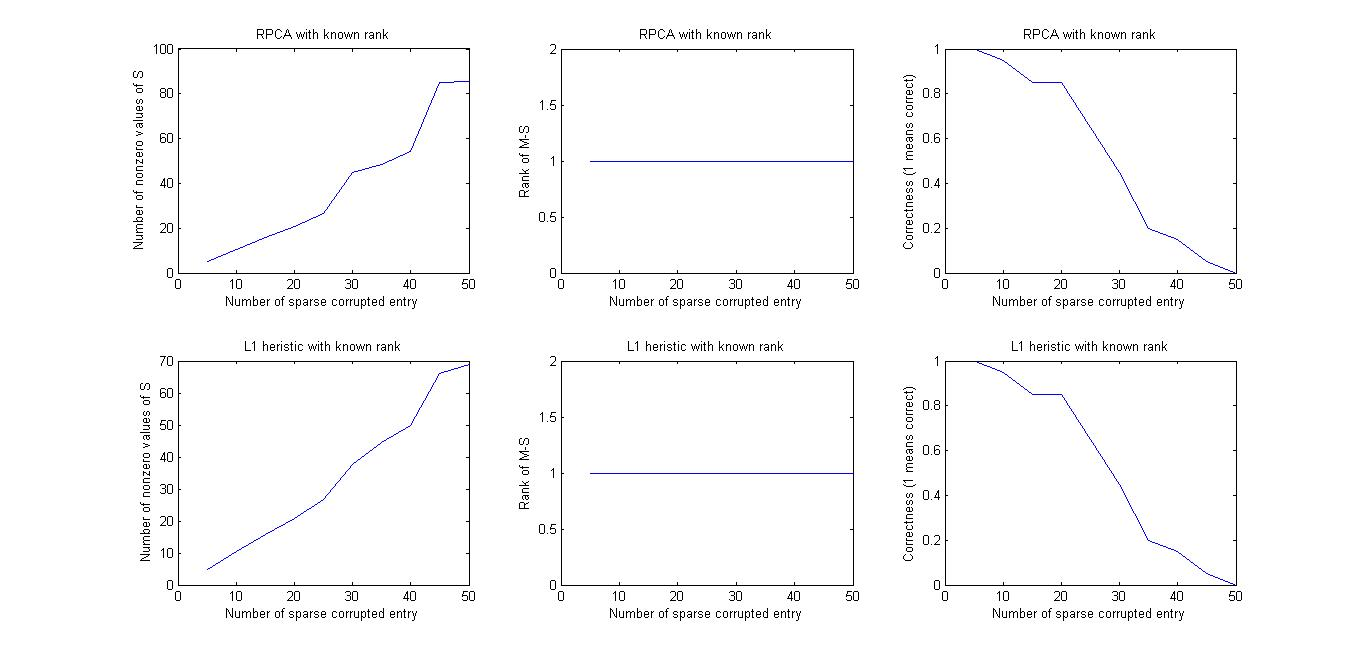
\includegraphics[width=16cm]{../figures/compare.jpg}
\end{figure}





%============================================================================================
%============================================================================================
\chapter{Algorithms}
%%%%%%%%%%%%%%%%%%%%%%%%%%%%%%%%%%%%%%%%%%%%%%%%%%%%%%%%%%%%
% EE227A Project: algorithms.tex
% Created by: Maximilian Balandat
% Last edited: Apr 02 2012
%%%%%%%%%%%%%%%%%%%%%%%%%%%%%%%%%%%%%%%%%%%%%%%%%%%%%%%%%%%%

% Use our own document class
\documentclass{../../common/projectreport}

% Input some of my LaTeX macros - Max
\newcommand{\norm}[3]{{\left\|#1\right\|}_{#2}^{#3}}
\newcommand{\normball}[2]{{\mathbb{B}_{#1}^{#2}}}
\newcommand{\proximal}[2]{{\prox_{#1}(#2)}}
\newcommand{\forAll}{{\forall \,}}
\newcommand{\Rbb}{{\mathbb R}}
\newcommand{\Rbf}{{\mathbf R}}
\newcommand{\Lhat}{{\hat{L}}}
\newcommand{\Shat}{{\hat{S}}}
\newcommand{\Yhat}{{\hat{Y}}}
\newcommand{\Xhat}{{\hat{X}}}
\newcommand{\Nbb}{{\mathbb N}}
\newcommand{\Fbb}{{\mathbb F}}
\newcommand{\Cbb}{{\mathbb C}}
\newcommand{\Tbb}{{\mathbb T}}
\newcommand{\Zbb}{{\mathbb Z}}
\newcommand{\etabar}{{\bar{\eta}}}
\newcommand{\kbar}{{\bar{k}}}
\newcommand{\rbar}{{\bar{r}}}
\newcommand{\xibar}{{\bar{\xi}}}
\newcommand{\ubar}{{\bar{u}}}
\newcommand{\vbar}{{\bar{v}}}
\newcommand{\uhat}{{\hat{u}}}
\newcommand{\vbf}{{\mathbf{v}}}
\newcommand{\vhat}{{\hat{v}}}
\newcommand{\xbar}{{\bar{x}}}
\newcommand{\xhat}{{\hat{x}}}
\newcommand{\xdot}{{\dot{x}}}
\newcommand{\Xdot}{{\dot{X}}}
\newcommand{\xtilde}{{\tilde{x}}}
\newcommand{\xtildedot}{{\dot{\tilde{x}}}}
\newcommand{\Phitilde}{{\tilde{\Phi}}}
\newcommand{\phat}{{\hat{p}}}
\newcommand{\shat}{{\hat{s}}}
\newcommand{\xbf}{{\mathbf{x}}}
\newcommand{\wbf}{{\mathbf{w}}}
\newcommand{\Pbf}{{\mathbf{P}}}
\newcommand{\Xbf}{{\mathbf{X}}}
\newcommand{\Ebf}{{\mathbf{E}}}
\newcommand{\Obf}{{\mathbf{0}}}
\newcommand{\ebf}{{\mathbf{e}}}
\newcommand{\alphabf}{{\mathbf{\alpha}}} 
\newcommand{\alphabar}{{\bar{\alpha}}} 
\newcommand{\sgn}{\text{sgn}}
\newcommand{\Range}{\mathcal{R}}
\newcommand{\Nullspace}{\mathcal{N}}

\newcommand{\pderiv}[2]{\frac{\partial #1}{\partial #2}}
\newcommand{\pderivsq}[2]{\frac{\partial^2 #1}{\partial #2^2}}
\newcommand{\pderivxy}[3]{\frac{\partial^2 #1}{\partial #2 \partial #3}}

\newcommand{\One}{{\mathbf{1}}}

\newcommand{\Ccal}{{\mathcal{C}}}
\newcommand{\Dcal}{{\mathcal{D}}}
\newcommand{\Fcal}{{\mathcal{F}}}
\newcommand{\Hcal}{{\mathcal{H}}}
\newcommand{\Lcal}{{\mathcal{L}}}
\newcommand{\Ncal}{{\mathcal{N}}}
\newcommand{\Pcal}{{\mathcal{P}}}
\newcommand{\Qcal}{{\mathcal{Q}}}
\newcommand{\Rcal}{{\mathcal{R}}}
\newcommand{\Scal}{{\mathcal{S}}}
\newcommand{\Tcal}{{\mathcal{T}}}
\newcommand{\Ucal}{{\mathcal{U}}}
\newcommand{\Xcal}{{\mathcal{X}}}
\newcommand{\Ycal}{{\mathcal{Y}}}


\newcommand{\ifthen}[2]{\textbf{if} #1 \textbf{then} #2}
\newcommand{\ifthenreturn}[2]{\textbf{if} #1 \textbf{then return} #2}
\newcommand{\then}[1]{\textbf{then} #1}
\newcommand{\return}[1]{\textbf{return} #1}
\newcommand{\returns}[1]{\textbf{returns} #1}
\newcommand{\thenreturn}[1]{\textbf{then return} #1}
\newcommand{\foreachindo}[3]{\textbf{for each} #1 \textbf{in} #2 \textbf{do} #3}
\newcommand{\algindent}[1]{\STATE\hspace{#1\algorithmicindent}}

\DeclareMathOperator{\blkdiag}{blkdiag}
\DeclareMathOperator{\trace}{\mathbf{Tr}}
\DeclareMathOperator{\Convh}{Conv}
\DeclareMathOperator{\rank}{rk}
\DeclareMathOperator{\diag}{diag}
\DeclareMathOperator{\Realpart}{Re}
\DeclareMathOperator{\Imagpart}{Im}
\DeclareMathOperator{\Poles}{Poles}
\DeclareMathOperator{\spanspace}{span}
\DeclareMathOperator*{\argmax}{arg\,max}
\DeclareMathOperator*{\argmin}{arg\,min}
\DeclareMathOperator{\Onebf}{{\mathbf{1}}}
\DeclareMathOperator{\dom}{dom}
\DeclareMathOperator{\grad}{\nabla\!\!}
\DeclareMathOperator{\epi}{epi}
\DeclareMathOperator{\sign}{sign}
\DeclareMathOperator{\divergence}{div}
\DeclareMathOperator{\prox}{prox}

\newcommand\independent{\protect\mathpalette{\protect\independenT}{\perp}}
\def\independenT#1#2{\mathrel{\rlap{$#1#2$}\mkern2mu{#1#2}}}


\newcommand{\Acal}{{\mathcal{A}}}
\newcommand{\Abar}{{\bar{A}}}


\theoremstyle{plain}
\newtheorem{thm}{Theorem}
\theoremstyle{plain}
\newtheorem{fact}[thm]{Fact}
\theoremstyle{plain}
\newtheorem{prop}[thm]{Proposition}




%%%%%%%%%%%%%%%%%%%%%%%%%%%%%%%%%%%%%%%%%%%%%%%%%%%%%%%%%%%%
\begin{document}


%%%%%%%%%%%%%%%%%%%%%%%%%%%%%%%%%%%%%%%%%%%%
\section{Overview}
\label{Algorithms:Overview:Sec}

This section discusses some of the algorithms that have recently been proposed in the literature to solve the Robust PCA problem
%
\begin{align}
\begin{split}
p^* = \min_{L,S} \; &\norm{L}{*}{} + \lambda \norm{S}{1}{} \\
\text{s.t.} \quad &M = L+S
\end{split}
\label{Algorithms:Overview:RecallRPCA}
\end{align}

There are various methods that can be used to solve~\eqref{Algorithms:Overview:RecallRPCA}. A straightforward way described in section~\ref{Algorithms:MainAlgs:IPM:Subsec} is to use general purpose interior point solvers~\cite{Sturm:1999uq,Toh:1999kx} to solve an SDP formulation of the dual of~\eqref{Algorithms:Overview:RecallRPCA}, an approach that works well for low-dimensional data~$M$ but unfortunately does not scale well. Another approach is to use iterative thresholding techniques as described in section~\ref{Algorithms:MainAlgs:ITM:Subsec}, which result in a very simple algorithm that can be applied also to high-dimensional data. Unfortunately the convergence of this algorithm is extremely slow. More sophisticated approaches include an accelerated proximal gradient algorithm (section~\ref{Algorithms:MainAlgs:PGM:Subsec}) and a gradient ascent algorithm applied to the dual problem of~\eqref{Algorithms:Overview:RecallRPCA} (section~\ref{Algorithms:MainAlgs:GAD:Subsec}). The current state of the art seems to be a adaptation of the Augmented Lagrangian Method to the non-smooth problem~\eqref{Algorithms:Overview:RecallRPCA}, an approach that is discussed in section~\ref{Algorithms:MainAlgs:AugLag:Subsec}.



%%%%%%%%%%%%%%%%%%%%%%%%%%%%%%%%%%%%%%%%%%%%
\section{Main algorithms for Robust PCA}
\label{Algorithms:MainAlgs:Sec}

%This section reviews a number of different approaches to solving the Robust PCA problem. 

%%%%%%%%%%%%%%%%%%%%%%%%%%%%
\subsection{Interior Point Methods}
\label{Algorithms:MainAlgs:IPM:Subsec}

As will be shown in the following section, the dual problem of~\eqref{Algorithms:Overview:RecallRPCA} can be cast as a Semidefinite Programming (SDP) problem for which a number of efficient polynomial-time interior-point solvers have been developed. In principle, one can then just apply these general purpose off-the-shelf solvers to the dual SDP. This approach will work well for small and medium sized problems, but unfortunately it does not scale with the size of the data matrix~$M$. The following section first develops the dual of the Robust PCA problem, section~\ref{Algorithms:MainAlgs:IPM:Complexity:Subsubsec} then discusses the limitations of using interior point methods on the resulting SDP. 


%%%%%%%%%%%%%%%%%
\subsubsection{Formulation of the Dual problem of Robust PCA as an SDP}
\label{Algorithms:MainAlgs:IPM:SDPform:Subsubsec}

Let us use the equality constraint to eliminate the variable~$L$ from~\eqref{Algorithms:Overview:RecallRPCA}. Using the facts that $\norm{X}{*}{} = \max_{\norm{Y}{2}{}\leq 1} \trace Y^T\!X$ and $\norm{X}{1}{} = \max_{\norm{Z}{\infty}{}\leq 1} \trace Z^T\!X$  the problem can be written as
%
\begin{align}
\begin{split}
p^* = \min_S \;\max_{Y,Z} \;\; &\trace Y^T(M-S) + \lambda \trace Z^TS \\
\text{s.t.} \quad & \norm{Y}{2}{}\leq 1 \\
&\norm{Z}{\infty}{}\leq 1
\end{split}
\label{Algorithms:MainAlgs:IPM:SDPform:NoNorms}
\end{align}
%
The dual function is 
\begin{align}
\begin{split}
g(Y,Z) &= \min_S \;\; \trace Y^T\!M + \trace (\lambda Z-Y)^T\!S \\
&= \begin{cases}
\trace Y^T\!M  & \text{ if } \; \lambda Z = Y \\
-\infty & \text{ otherwise }
\end{cases} 
\end{split}
\label{Algorithms:MainAlgs:IPM:SDPform:DualFunct}
\end{align}
%
We obtain the dual problem 
\begin{align}
\begin{split}
p^* \geq d^* = \max_{Y,Z} \;\; &\trace Y^T\!M \\
\text{s.t.} \quad & \lambda Z = Y \\
&\norm{Y}{2}{}\leq 1 \\
&\norm{Z}{\infty}{}\leq 1
\end{split}
\label{Algorithms:MainAlgs:IPM:SDPform:DualProb}
\end{align}
%
which after eliminating the variable~$Z$ and using homogeneity of the norm becomes
\begin{align}
\begin{split}
d^* = \max_{Y} \;\; &\trace Y^T\!M \\
\text{s.t.} \quad & \norm{Y}{2}{}\leq 1 \\
&\norm{Y}{\infty}{}\leq \lambda
\end{split}
\label{Algorithms:MainAlgs:IPM:SDPform:DualSimpler}
\end{align}

Noting that $\norm{Y}{2}{}\leq 1 \; \Longleftrightarrow \; I-X^T(I)^{-1}X \succeq 0$ and using a Schur Complement lemma, the dual problem can be transformed into the following SDP standard form:
\begin{align}
\begin{split}
d^* = \max_{Y} \;\; &\trace M^T\!Y \\ 
\text{s.t.} \quad &\begin{bmatrix} I & Y^T \\ Y & I \end{bmatrix} \succeq 0 \\
&\trace \Delta_{ij}^TY \leq \lambda, \quad i = 1,\dotsc, m, \; j=1,\dotsc,n \\
&\trace \Delta_{ij}^TY \geq -\lambda, \quad i = 1,\dotsc, m, \; j=1,\dotsc,n
\end{split}
\label{Algorithms:MainAlgs:IPM:SDPform:DualSDP}
\end{align}
%
Here $\Delta_{ij} \in \Rbf^{m\times n}$ is such that $\Delta_{ij}(k,l) = \delta_{ik}\delta_{jl}$. Note that both primal and dual problem are (trivially) strictly feasible. In fact, the primal is unconstrained and an obvious strictly feasible dual variable is~$Y=0$. Hence strong duality holds ($p^* = d^*$) and both primal and dual problem are attained.\\

\textbf{Recovering the primal solution}

To recover the primal solution we can distinguish the two cases $\lambda \leq 1$ and $\lambda >1$. For the latter one, first note that $\norm{Y}{\infty}{} \leq \norm{Y}{2}{}$ for all~$Y$. To show this first recall that $c := \norm{Y}{2}{} = \max_{\norm{x}{2}{}=1} \norm{Yx}{2}{}$. This means that $c - x^TY^TYx \geq0, \,\forAll x$ or, equivalently, $cI-Y^TY \succeq 0$. Using a Schur Complement this can be written as
%
\begin{align*}
\begin{bmatrix} I & Y \\Y^T & cI \end{bmatrix} \succeq 0
\end{align*}
It is easy to see that this implies that  
\begin{align*}
\begin{bmatrix} 1 & Y_{ij} \\Y_{ij} & c \end{bmatrix} \succeq 0
\end{align*}
for all $i,j$, which is equivalent to $|Y_{ij}| \leq c,\; \forAll i,j$. This shows that $\norm{Y}{\infty}{} \leq \norm{Y}{2}{}$.

Hence we observe that if $\lambda >1$ the constraint $\norm{Y}{2}{} \leq \lambda$ will be inactive, that is $|Y_{ij}|<\lambda,\;\forAll i,j$. Therefore, for $\lambda > 1$, removing this constraint from~\eqref{Algorithms:MainAlgs:IPM:SDPform:DualSimpler} does not change the problem. We have $d^* = \max_{\norm{Y}{2}{}\leq 1} \trace Y^T\!M = \norm{M}{*}{}$, and this lower bound is achieved by the primal (feasible) solution $L=M$ and $S =0$.

If $\lambda \leq 1$, then ....

%If we then dualize the resulting problem, we obtain 
%\begin{align}
%\begin{split}
%p^*&=\max_{Y} \;\;\min_{\gamma\geq0}\;\; \trace Y^T\!M - \gamma \left(\min_{\norm{X}{*}{}\leq 1}\trace Y^T\!X-1\right) \\
%&= \min_{\gamma\geq0}\;\;\max_{Y,\norm{X}{*}{}\leq 1}\;\; \trace Y^T\!M + \gamma \left( 1- \trace Y^T\!X \right) \\
%&= \min_{\gamma\geq0}\;\;\max_{Y,\norm{X}{*}{}\leq 1}\;\; \trace Y^T\!(M -\gamma X) + \gamma 
%\end{split}
%\label{Algorithms:MainAlgs:IPM:SDPform:DualLambdaBig}
%\end{align}
%
%Lagrangian stationarity then implies that 
%
%If we dualize the constraint  of





%%%%%%%%%%%%%%%%%
\subsubsection{Using Interior Point Methods to Solve the Dual}
\label{Algorithms:MainAlgs:IPM:Complexity:Subsubsec}

Problem~\eqref{Algorithms:MainAlgs:IPM:SDPform:DualSimpler} is an SDP and can therefore in principle be solved using off-the-shelf solver packages like~\cite{Sturm:1999uq} and~\cite{Toh:1999kx}. These solvers are based on interior point methods which offer superior convergence rates~\cite{Boyd:2004aa} but unfortunately do not scale particularly well with the size of the matrix~$M$. The reason for this is that the computation of the step direction relies on second-order information of the (barrier-augmented) objective function, the computation of which is infeasible when the number of variables is very high. For applications that involve large-scale data matrices (with~$m$ in the thousands or even millions), the use interior point methods therefore quickly becomes infeasible. In order to overcome this scalability issue, a variety of first-order methods exploiting the particular structure of the Robust PCA problem have been proposed. Some of these methods will be described in the following.

%A bottleneck in higher dimensions is in particular the complexity of computing the Newton step direction, which is~$O(m^6)$ (CHECK THIS, PROVIDE REFERENCE). For applications that involve large-scale data matrices (with~$m$ in the thousands or even millions), the use interior point methods therefore quickly becomes infeasible.
%
%%The SDP formulation~\eqref{Algorithms:MainAlgs:IPM:SDPform:DualSDP} of the dual problem involves only the matrix variable~$Y\in\Rbf^{m\times n}$, hence the problem involves~$mn$ scalar variables. There are~$2mn$ scalar constraints (due to the constraint on the~$\infty$-norm) and a positive semidefiniteness constraint on a square matrix of dimension $m+n$ (due to the constraint on the operator norm). 
%
%The reason why interior point solvers do not scale well with the matrix size is because generally the computation of the step direction relies on second-order information of the objective function, the computation of which is infeasible when the number of variables is very high. In order to overcome this scalability issue, a variety of first-order methods exploiting the particular structure of the Robust PCA problem have been proposed. Some of these methods are described will be described in the following.


%%%%%%%%%%%%%%%%%%%%%%%%%%%%
\subsection{Iterative Thresholding Method}
\label{Algorithms:MainAlgs:ITM:Subsec}

Among the first techniques used to solve~\eqref{Algorithms:Overview:RecallRPCA} for high-dimensional data was an adaptation \cite{Wright:2009fk}\footnote{note that the iterative thresholding algorithm seems to never have appeared in the published version of~\cite{Wright:2009fk}, which instead contains the accelerated proximal gradient method described in section~\ref{Algorithms:MainAlgs:PGM:Subsec}} of an iterative thresholding method originally proposed for the matrix completion problem in~\cite{Cai:2010uq}. For this method the authors of consider a relaxation of the original problem~\eqref{Algorithms:Overview:RecallRPCA} of the form 
%
\begin{align}
\begin{split}
\min_{L,S} \;\; &\norm{L}{*}{} + \lambda \norm{S}{1}{} + \frac{1}{2\tau} \norm{L}{F}{2} + \frac{1}{2\tau} \norm{S}{F}{2} \\
\text{s.t.} \quad &M=L+S
\end{split}
\label{Algorithms:MainAlgs:ITM:Relax}
\end{align}
%
where $\tau \gg 1$ is a scalar parameter. Generalizing the result from~\cite{Cai:2010uq} (which considers the matrix completion problem, i.e. $S=0$), the authors of~\cite{Wright:2009fk} argue that for large values of~$\tau$ the solution of~\eqref{Algorithms:MainAlgs:ITM:Relax} will be very close to that of~\eqref{Algorithms:Overview:RecallRPCA} (but interestingly enough they do not prove it!). One can now use iterative thresholding techniques to solve~\eqref{Algorithms:MainAlgs:ITM:Relax}. Although the resulting algorithm has little relevance in practice because of its extremely slow convergence, we will see in the following sections that its main ideas are the basis for a number of other similar algorithms. Therefore we briefly describe the iterative thresholding algorithm here.\\ 

The Lagrangian of the problem~\eqref{Algorithms:MainAlgs:ITM:Relax} is given by
%
\begin{align}
\Lcal(L,S,Y) = \norm{L}{*}{} + \lambda \norm{S}{1}{} + \frac{1}{2\tau} \norm{L}{F}{2} + \frac{1}{2\tau} \norm{S}{F}{2} + \frac{1}{\tau} \langle Y, M-L-S \rangle
\label{Algorithms:MainAlgs:ITM:Lagr}
\end{align}
%
The idea of the iterative thresholding algorithm is, as the name suggests, to update the variables $L,S$ and $Y$ iteratively. More specifically, the Lagrangian $\Lcal(L,S,Y)$ is minimized w.r.t $L$ and $S$ for some fixed dual variable~$Y$, and the violation of the constraint is then used to update~$Y$ using the gradient step~$Y^+ = Y + t (M-L-S)$, where~$0<t<1$ is the step size.\\

Note that for fixed~$Y$ we have
%
\begin{align}
\begin{split}
(\Lhat,\Shat) :&= \argmin_{L,S} \; \Lcal(L,S,Y) \\
&= \argmin_{L,S} \; \norm{L}{*}{} + \lambda \norm{S}{1}{} + \frac{1}{2\tau} \norm{L}{F}{2} + \frac{1}{2\tau} \norm{S}{F}{2} + \frac{1}{\tau} \langle Y, M-L-S \rangle \\
&= \argmin_{L,S} \; \norm{L}{*}{} + \lambda \norm{S}{1}{} + \frac{1}{2\tau} \norm{L-Y}{F}{2} + \frac{1}{2\tau} \norm{S-Y}{F}{2}
\end{split}
\label{Algorithms:MainAlgs:ITM:ArgminLagr}
\end{align}
%
We note that the above problem is completely separable hence the minimizers~$\Lhat$ and~$\Shat$ can be determined independently. Using optimality conditions based on the subgradient it can be shown~\cite{Cai:2010uq,Wright:2009fk} that the minimizers~$\Lhat$ and~$\Shat$ are both of a simple form. To this end, consider the following 
% where~$\Scal_\varepsilon[X]$ is the 
extension to the matrix case of the well known soft-thresholding operator (e.g. from the proximal mapping of the~$l_1$-norm in the vector case):
%
\begin{align}
\left(\Scal_\varepsilon[X]\right)_{ij} := \begin{cases} x_{ij}-\varepsilon & \text{ if} \;\; x_{ij}>\varepsilon \\ x_{ij}+\varepsilon & \text{ if} \;\; x_{ij}<-\varepsilon \\ 0 & \text{ otherwise} \end{cases}
\label{Algorithms:MainAlgs:ITM:Shrink}
\end{align}


\begin{theorem}[Singular Value Thresholding~\cite{Cai:2010uq}]
For each $\tau \geq 0$ and $Y\in \Rbf^{m\times n}$, we have that
\begin{align}
\Dcal_\tau(Y) := U \Scal_\tau[\Sigma] V^T = \argmin_X \; \norm{X}{*}{} + \frac{1}{2\tau} \norm{X-Y}{F}{2}
\label{Algorithms:MainAlgs:ITM:SVTtheore:eq}
\end{align}
where $Y = U\Sigma V^*$ is the SVD of~$Y$.
\label{Algorithms:MainAlgs:ITM:SVTtheorem}
\end{theorem}

Since Theorem~\ref{Algorithms:MainAlgs:ITM:SVTtheorem} is central to all algorithms discussed in this chapter, we give its proof here.
%
\begin{proof}[Proof of Theorem~\ref{Algorithms:MainAlgs:ITM:SVTtheorem}] 
Since the objective function $f_0(X) := \argmin_X \; \norm{X}{*}{} + \frac{1}{2\tau} \norm{X-Y}{F}{2}$ is strictly convex its minimizer is unique. Recall that $Z$ is a subgradient of a convex function $f:\Rbf^{m\times n} \mapsto \Rbf$ at $X_0$ if $f(X) \geq f(X_0) + \langle Z,X-X_0\rangle$ for all~$X$. The set of all sugradients~$Z$ at $X_0$ is called the subdifferential and denoted $\partial f(X_0)$. By definition it follows that $\Xhat$ minimizes $f_0$ if and only if $0$ is as subgradient of $f_0$ at $\Xhat$. Using standard subgradient calculus this translates to $0 \in \Xhat - Y + \tau \partial ||\Xhat||_{*}$, where $\partial ||\Xhat||_{*}$ is the subdifferential of the nuclear norm at $\Xhat$. To show that $\Dcal_\tau(Y)$ satisfies~\eqref{Algorithms:MainAlgs:ITM:SVTtheore:eq} we therefore need to show that $0 \in \Dcal_\tau(Y)  - Y + \tau \partial ||\Dcal_\tau(Y) ||_{*}$.  

Let $X\in \Rbf^{m\times n}$ be arbitrary Let $U\Sigma V^*$ be its SVD. It can be shown that 
\begin{align*}
\partial ||X||_{*} = \left\{ UV^*+W \,\mid\, W\in \Rbf^{m\times n},\; U^*W =0,\; WV =0,\; \norm{W}{2}{}\leq 1 \right\}
\end{align*}
To use the above result decompose the SVD of~$Y$ as $Y = U_0\Sigma_0V_0^* + U_1\Sigma_1V_1^*$, where $U_0,V_0$ ($U_1,V_1$) are the singular vectors associated with singular values greater (less or equal) than~$\tau$. With this notation we have $\Dcal_\tau(Y) = U_0(\Sigma_0-\tau I)V_0^*$,  so $Y-\Dcal_\tau(Y) = \tau (U_0V_0^*+W)$ with $W=\tau^{-1}U_1\Sigma_1V_1^*$. By definition of the SVD $U_0^*W=0$ and $WV_0=0$. Furthermore, since $\max(\Sigma_1) \leq \tau$ it also holds that $\norm{W}{2}{}\leq 1$. Together this shows that $Y - \Dcal_\tau(Y) \in \tau \partial ||\Dcal_\tau(Y) ||_{*}$.
\end{proof}


It is also not hard to find the minimizer~$\Shat$ of~\eqref{Algorithms:MainAlgs:ITM:Lagr}, as the following proposition shows:

\begin{proposition}[Matrix Value Thresholding]
For each $\tau,\lambda \geq 0$ and $Y\in \Rbf^{m\times n}$, we have that
\begin{align}
\Scal_{\tau\lambda}[Y] = \argmin_X \; \lambda \norm{X}{1}{} + \frac{1}{2\tau} \norm{X-Y}{F}{2}
\label{Algorithms:MainAlgs:ITM:MVTprop:eq}
\end{align}
\label{Algorithms:MainAlgs:ITM:MVTprop}
\end{proposition}

\begin{proof}[Proof of Proposition~\ref{Algorithms:MainAlgs:ITM:MVTprop}] 
Note that the objective function $h_0(X) := \lambda \norm{X}{1}{} + \frac{1}{2\tau} \norm{X\!-\!Y}{F}{2}$ in~\eqref{Algorithms:MainAlgs:ITM:MVTprop:eq} is completely decomposable and can be written in the form $h_0(X) = \sum_{i,j} \lambda |X_{ij}| + \frac{1}{2\tau} (X_{ij}\!-\!Y_{ij})^2$, so the minimization over $X$ can be carried out element-wise. Using the same reasoning as in the proof of Theorem~\ref{Algorithms:MainAlgs:ITM:SVTtheorem}, we have that the element $X_{ij}$ is a minimizer if and only if $0 \in \partial h_0(X)$. This condition can be written as $Y_{ij}-X_{ij} \in \tau \lambda\, \partial |X_{ij}|$. We consider the cases $X_{ij} =0$ and $X_{ij} \neq 0$. If $X_{ij} =0$ then the condition reads $Y_{ij} \in \tau \gamma [-1,1]$. In other words, when $|Y_{ij}| \leq \tau \gamma$ then $X_{ij}=0$. On the other hand, if $X_{ij} \neq 0$, then  $\partial \, |X_{ij}| = \sign(X_{ij})$ and we have $X_{ij}= Y_{ij} -\tau\lambda \sign(Y_{ij})$, which is in fact the soft-thresholding operator $\Scal_{\tau\lambda}[X_{ij}]$.
\end{proof}


Applying Theorem~\ref{Algorithms:MainAlgs:ITM:SVTtheorem} and Proposition~\ref{Algorithms:MainAlgs:ITM:MVTprop} to~\eqref{Algorithms:MainAlgs:ITM:ArgminLagr} we find that the minimizers~$\Lhat$ and~$\Shat$ of~\eqref{Algorithms:MainAlgs:ITM:Lagr} are given, respectively, by 
%
\begin{align}
\Lhat &= U \Scal_\tau[\Sigma] V^T
\label{Algorithms:MainAlgs:ITM:ArgminLhat} \\
\Shat &= \Scal_{\tau\lambda}[Y]
\label{Algorithms:MainAlgs:ITM:ArgminShat}
\end{align}
%
%
The overall iterative thresholding algorithm for Robust PCA is given in Algorithm~\ref{Algorithms:MainAlgs:ITM:Algorithm}. 
%
\begin{algorithm}
\caption{Iterative Thresholding Algorithm}
\KwIn{Observation matrix~$M$, parameters~$\lambda,\tau$}
initialization: $k=0$, $Y_0 = 0$\;
\While{not converged}{
$k=k+1$\;
$(U,\Sigma,V) = \text{svd}(Y_{k-1})$\;
$L_k = U \Scal_\tau[\Sigma] V^T$\;
$S_k = \Scal_{\lambda\tau}[Y_{k-1}]$\;
$Y_k = Y_{k-1} + t_k (M-L_k-S_k)$\;
}
\KwOut{$L=L_k$, $S=S_k$}
\label{Algorithms:MainAlgs:ITM:Algorithm}
\end{algorithm}

Algorithm~\ref{Algorithms:MainAlgs:ITM:Algorithm} is extremely simple to implement, as each iteration only requires the computation of an SVD of the current dual variable~$Y_k$ and a few elementary matrix operations. Note that, in fact, since the shrinking operator sets all singular values less than the threshold parameter to zero one really only needs to compute the singular values that lie above this threshold. However, while this iterative thresholding scheme is very simple and has been proved to converge, its convergence unfortunately is extremely slow. The authors of~\cite{Wright:2009fk} found that it typically requires about~$10^4$ iterations to converge for problems of reasonable size. Furthermore it is hard to find good general schemes to optimize the choice of the step size~$t_k$~\cite{Lin:2010fk}. Therefore the practical applicability of this approach is limited.


%%%%%%%%%%%%%%%%%%%%%%%%%%%%
\subsection{Accelerated Proximal Gradient Method}
\label{Algorithms:MainAlgs:PGM:Subsec}

An accelerated proximal gradient (APG) method for solving~\eqref{Algorithms:Overview:RecallRPCA} was proposed in~\cite{Lin:2009kx}. The method is essentially an application of the FISTA algorithm~\cite{Beck:2009kx} to a relaxation of the original RPCA problem in combination with a continuation technique. This FISTA algorithm algorithm is reminiscent of Nesterov's ``optimal'' first-oder method for smooth objective functions~\cite{Nesterov:1983uq}, whose~$O(1/k^2)$ convergence rate result was extended to non-smooth objectives in~\cite{Nesterov:2007kx}. Besides being theoretically appealing, the APG method is also in practice much faster than the iterative thresholding algorithm discussed in section~\ref{Algorithms:MainAlgs:ITM:Subsec}.\\

The following sections describe the APG algorithm. As in~\cite{Lin:2009kx} we first give a general formulation and then show how it can be applied to the Robust PCA problem, using ideas from section~\ref{Algorithms:MainAlgs:ITM:Subsec}.


%%%%%%%%%%%%%%%%%
\subsubsection{A General Form of the Accelerated Proximal Gradient Method}
\label{Algorithms:MainAlgs:PGM:General:Subsubsec}

Proximal gradient algorithms in general can be used to solve unconstrained problems of the form 
%
\begin{align}
\min_{x} \;\; &f(x) := g(x) + h(x)
\label{Algorithms:MainAlgs:PGM:General:GenPGA}
\end{align}
%
where~$g$ is convex and differentiable and~$h$ is closed\footnote{that is, its epigraph is closed}, convex but need not be differentiable. The proximal mapping of a convex function~$h$ is defined as
%
\begin{align}
\proximal{h}{x} := \argmin_u \left( h(u) + \frac{1}{2}\norm{u-x}{}{2} \right)
\label{Algorithms:MainAlgs:PGM:General:proxmapping}
\end{align}
%
Here $\norm{\cdot}{}{}$ denotes the inner product norm\footnote{Note that the derivation holds for real inner product spaces, not just~$\Rbf^n$. We are particularly interested in the case~$\Rbf^{m\times n}$}. Note that since~$h$ is convex and the norm is strictly convex, the optimizer in~\eqref{Algorithms:MainAlgs:PGM:General:proxmapping} is unique. The step of each iteration of the classic (non-accelerated) proximal gradient algorithm is
%
\begin{align}
x^+ = \proximal{\delta h}{x-\delta \nabla g(x)}
\label{Algorithms:MainAlgs:PGM:General:proxAlg}
\end{align}
%
where~$x^+$ denotes the next iterate, based on the current iterate~$x$, and~$\delta$ is the step size (which can be fixed or determined via backtracking line search). Since the proximal mapping~\eqref{Algorithms:MainAlgs:PGM:General:proxAlg} needs to be computed at each iteration (possibly multiple times because of the line search), the algorithm is most effective when this can be done cheaply. Depending on the function~$h$, the proximal gradient algorithm can be seen as a generalization of different gradient-based algorithms. In particular, for~$h(x) \equiv 0$ the standard gradient algorithm is recovered and for~$h(x) = I_C(x)$, where $I_C$ denotes the indicator function for the convex set~$C$, the projected gradient algorithm is recovered. 

Note that~\eqref{Algorithms:MainAlgs:PGM:General:proxAlg} can be written as
%
\begin{align}
\begin{split}
x^+ &= \argmin_u \left( h(u) + \frac{1}{2\delta}\norm{u-x+\delta\nabla g(x)}{}{2} \right) = \argmin_u \left( h(u) +\frac{1}{2\delta} \norm{u-G(x)}{}{2} \right) \\
&= \argmin_u \left( h(u) +g(x) + \langle \nabla g(x),u-x\rangle + \frac{1}{2\delta}\norm{u-x}{}{2} \right)
\end{split}
\label{Algorithms:MainAlgs:PGM:General:proxAlgRewritten}
\end{align}
%
where $G(x) := x-\delta\grad g(x)$. Therefore, each step~\eqref{Algorithms:MainAlgs:PGM:General:proxAlg} can be interpreted as minimizing the function~$h(u)$ plus a quadratic local model of~$g(u)$ around the current iterate~$x$. This classic form of the proximal gradient algorithm is well known in the literature and, under Lipschitz continuity of the gradient of~$g$ and some technical conditions on the step size~$t$, has been shown to have a convergence rate no worse than~$O(1/k)$ (PUT REFERENCE). In particular, a popular choice for~$\delta$ is the fixed step size $\delta = 1/L_g$, where~$L_g$ is a Lipschitz constant of the gradient of~$g$, that is we have $\norm{\grad g(x) -\grad g(y)}{}{} \leq L_g \norm{x-y}{}{}$ for all~$x,y$. Note that in practice for a general problem the value of~$L_g$ might be unknown. This is not a big concern for the type of problem arising in Robust PCA, hence we will assume this choice of~$\delta=1/L_g$ in the following.

It turns out that the choice for the point around which the quadratic local model of~$g(u)$ is constructed has an important effect on the convergence rate, and that less obvious choices than just the previous iterate~$x$ are actually better (in the sense that they yield higher convergence rates). Specifically, consider a generalized version of~\eqref{Algorithms:MainAlgs:PGM:General:proxAlgRewritten}, where the approximation of~$g$ is constructed around some~$y$ that may depend on all prior iterates~$x_0,\dotsc,x_k$:
%
\begin{align}
x^+ &= \argmin_u \left( h(u) +\frac{L_g}{2} \norm{u-G(y)}{}{2} \right)
\label{Algorithms:MainAlgs:PGM:General:proxAlgGeneralized}
\end{align}
%
Nesterov in~\cite{Nesterov:1983uq} showed that in the smooth case the standard gradient algorithm (i.e.~$h(x) \equiv 0$) can be accelerated by choosing $y_k = x_k + \frac{t_{k-1}-1}{t_k}(x_k-x_{k-1})$, leading to a theoretical convergence rate of~$O(1/k^2)$. This algorithm is optimal in the sense that its convergence rate achieves (in terms of order) the theoretical complexity bound on all first order algorithms. The seminal work~\cite{Nesterov:1983uq} has been extended to the non-smooth case in~\cite{Beck:2009kx,Nesterov:2007kx}, yielding the generic accelerated proximal gradient method given in Algorithm~\ref{Algorithms:MainAlgs:PGM:General:Algorithm}.
%
\begin{algorithm}
\caption{Accelerated Proximal Gradient Algorithm}
initialization: $k=0$, $t_0=t_{-1} = 1$\;
\While{not converged}{
$y_k = x_k + \frac{t_{k-1}-1}{t_k} (x_k-x_{k-1})$\;
$G_k = y_k - \frac{1}{L_g} \grad g(y_k) $\;
$x_{k+1} = \argmin_x \left( h(x) +\frac{L_g}{2} \norm{x-G(y_k)}{}{2} \right) $\;
$t_{k+1} = \frac{1+\sqrt{4t_k^2+1}}{2}$\;
$k=k+1$\;
}
\label{Algorithms:MainAlgs:PGM:General:Algorithm}
\end{algorithm}



%%%%%%%%%%%%%%%%%
\subsubsection{Accelerated Proximal Gradient Algorithm Applied to Robust PCA}
\label{Algorithms:MainAlgs:PGM:APGRPCA:Subsubsec}

Using some the ideas from the iterative thresholding method in section~\ref{Algorithms:MainAlgs:ITM:Subsec}, it is possible to construct an accelerated proximal gradient algorithm for a relaxation of the original problem~\eqref{Algorithms:Overview:RecallRPCA}. In particular, it is easy to see that in the common case~$h(x) = \norm{x}{1}{}$ the update for~$x$ in Algorithm~\ref{Algorithms:MainAlgs:PGM:General:Algorithm} is simply given by $x_{k+1} = \Scal_{1/L_g}[G(y_k)]$, where~$\Scal_\varepsilon$ is the soft-thresholding operator defined in~\eqref{Algorithms:MainAlgs:ITM:Shrink}. Similar ideas can be used to develop an APG algorithm for the Robust PCA problem. 

The authors of~\cite{Lin:2009kx} consider a relaxation of~\eqref{Algorithms:Overview:RecallRPCA} of the form
%
\begin{align}
\min_{L,S} \;\; &\mu \norm{L}{*}{} + \mu \lambda \norm{S}{1}{} + \frac{1}{2} \norm{L+S-M}{F}{2} 
\label{Algorithms:MainAlgs:PGM:APGRPCA:Relax}
\end{align}
%
It can be shown that for~$\mu \rightarrow 0$, any solution of~\eqref{Algorithms:MainAlgs:PGM:APGRPCA:Relax} approaches the solution set of~\eqref{Algorithms:Overview:RecallRPCA}. In practice, rather than fixing~$\mu$ to some small value, one can achieve superior convergence of the algorithm by using a continuation technique on~$\mu$, that is, by solving~\eqref{Algorithms:MainAlgs:PGM:APGRPCA:Relax} by repeatedly decreasing the value of~$\mu$ in the steps of the accelerated proximal gradient algorithm. This can be interpreted as a particular homotopy method. 

With $X=(L,S)$ we identify $h(X) = \mu \norm{L}{*}{} + \mu \lambda \norm{S}{1}{}$ and $g(X) = \frac{1}{2} \norm{L+S-M}{F}{2}$ in~\eqref{Algorithms:MainAlgs:PGM:APGRPCA:Relax}. The gradient of~$g$ is $\nabla g(X) = (\nabla_{\!L} g(X),\nabla_{\!S} g(X))$, where $\nabla_{\!L} g(X) = \nabla_{\!S} g(X) = L+S-M$. Thus
\begin{align*}
\norm{\grad g(X_1) -\grad g(X_2)}{}{} &= \norm{\begin{bmatrix} L_1+S_1-M \\ L_1+S_1-M  \end{bmatrix} - \begin{bmatrix} L_2+S_2-M \\ L_2+S_2-M  \end{bmatrix}}{}{} = \norm{\begin{bmatrix} L_1-L_2 + S_1-S_2 \\ L_1-L_2 + S_1-S_2  \end{bmatrix}}{}{} \\
&\leq \norm{\begin{bmatrix} L_1-L_2\\ S_1-S_2  \end{bmatrix}}{}{} + \norm{\begin{bmatrix} S_1-S_2\\ L_1-L_2  \end{bmatrix}}{}{} = 2\, \norm{X_1-X_2}{}{}
\end{align*}
which means that a Lipschitz constant is given by $L_g =2$. It turns out that because of the separability of both the function~$h$ and the Frobenius norm the update can be be decomposed as follows:
%
\begin{align*}
(L_{k+1},S_{k+1}) &= X_{k+1} = \argmin_X \left( h(X) +\frac{L_g}{2} \norm{X-G(Y_k)}{}{2} \right)  \\
&= \argmin_{L,S} \left( \mu \norm{L}{*}{} + \mu \lambda \norm{S}{1}{} + \norm{\begin{bmatrix}L \\ S\end{bmatrix} - \begin{bmatrix}G_k^L \\ G_k^S\end{bmatrix} }{}{2} \right) \\
&= \argmin_{L,S} \left( \norm{L}{*}{} + \frac{1}{2\frac{\mu}{2}} \norm{L - G_k^L}{}{2}  + \lambda \norm{S}{1}{}  + \frac{1}{2\frac{\mu}{2}}  \norm{S - G_k^S}{}{2} \right)
\end{align*}
The problem is therefore completely separable and clearly the sum of two problems of the form~\eqref{Algorithms:MainAlgs:PGM:General:GenPGA}. In particular, if $G_k^L = U \Sigma V^T$ is the SVD of~$G_k^L$ then, using the results from section~\ref{Algorithms:MainAlgs:ITM:Subsec}, the iterates~$L_{k+1}$ and $S_{k+1}$ are given by 
\begin{align}
L_{k+1} &= U \Scal_\frac{\mu}{2}[\Sigma] V^T \label{Algorithms:MainAlgs:PGM:APGRPCA:LIterate} \\
S_{k+1} &= \Scal_\frac{\lambda\mu}{2}[G_k^S] \label{Algorithms:MainAlgs:PGM:APGRPCA:SIterate}
\end{align}
Therefore it is rather straightforward to formulate a version Algorithm~\ref{Algorithms:MainAlgs:PGM:General:Algorithm} for the Robust PCA problem. One extension to Algorithm~\ref{Algorithms:MainAlgs:PGM:General:Algorithm} is the use of a continuation technique (or homotopy method) for the parameter~$\mu$. In~\cite{Lin:2009kx}, the authors propose to start from some large value~$\mu_0$ and then choose~$\mu_{k+1} = \max(\eta \mu_k,\bar{\mu})$, where $0<\eta<1$ and $\bar{\mu}$ is a lower limit on~$\mu_k$. This continuation technique has been observed to improve convergence. The Accelerated Proximal Gradient Algorithm applied to the Robust PCA problem is given in Algorithm~\ref{Algorithms:MainAlgs:PGM:APGRPCA:Algorithm}.
%
\begin{algorithm}
\caption{Accelerated Proximal Gradient Algorithm for Robust PCA}
\KwIn{Observation matrix~$M$, parameter~$\lambda$}
initialization: $k=0$, $L_0=L_{-1}=0$, $S_0=S_{-1}= 0$, $t_0=t_{-1} = 1$, $\bar{\mu} = \delta \mu_0$\;
\While{not converged}{
$Y_k^L = L_k + \frac{t_{k-1}-1}{t_k} (L_k-L_{k-1})$, $\; Y_k^S = S_k + \frac{t_{k-1}-1}{t_k} (S_k-S_{k-1})$\;
$G_k^L = Y_k^L -\frac{1}{2} (Y_k^L+Y_k^S-M)$\;
$(U,\Sigma,V) = \text{svd}(G_{k}^L)$, $L_{k+1} = U \Scal_{\mu_k/2}[\Sigma] V^T$\;
$G_k^S = Y_k^S -\frac{1}{2} (Y_k^L+Y_k^S-M)$\;
$S_{k+1} = \Scal_{\lambda\mu_k/2}[G_{k}^S]$\;
$t_{k+1} = \frac{1+\sqrt{4t_k^2+1}}{2}$\;
$\mu_{k+1} = \max(\eta \mu_k,\bar{\mu})$\;
$k=k+1$\;
}
\KwOut{$L=L_k$, $S=S_k$}
\label{Algorithms:MainAlgs:PGM:APGRPCA:Algorithm}
\end{algorithm}

We will restate the main convergence theorem for Algorithm~\ref{Algorithms:MainAlgs:PGM:APGRPCA:Algorithm} without proof. 

\begin{theorem}[\cite{Lin:2010fk}]
Let $F(X) = F(L,S) := \bar{\mu} \norm{L}{*}{} + \bar{\mu} \lambda \norm{S}{1}{} + \frac{1}{2} \norm{L+S-M}{F}{2}$. Then for all $k>k_0 := -C_1\log(\eta)$ it holds that
\begin{align*}
F(X_k) - F(X^*) \leq \frac{4\norm{C_{k_0}-X^*}{F}{2}}{(k-k_0+1)^2}
\end{align*}
where~$C_1 = \log(\mu_0/\bar{\mu})$ and $X^*$ is any solution to~\eqref{Algorithms:MainAlgs:PGM:APGRPCA:Relax}.
\end{theorem}


\begin{remark}[Accuracy of the APG method]
Note that for any finite $\bar{\mu}$ Algorithm~\ref{Algorithms:MainAlgs:PGM:APGRPCA:Algorithm} provides only an approximate solution of the Robust PCA problem due to the replacement of the equality constraint with the penalty term $\frac{1}{2\bar{\mu}} \norm{L+S-M}{F}{2}$.
\end{remark}


%%%%%%%%%%%%%%%%%%%%%%%%%%%%
\subsection{Gradient Ascent on the Dual}
\label{Algorithms:MainAlgs:GAD:Subsec}

In section~\ref{Algorithms:MainAlgs:IPM:Complexity:Subsubsec} we discussed why solving the Robust PCA dual problem~\eqref{Algorithms:MainAlgs:IPM:SDPform:DualSimpler} via interior point techniques quickly becomes infeasible with growing size of the data matrix~$M$. Another way of solving the dual given in~\cite{Lin:2009kx} is based on a steepest ascent algorithm. Note that the dual problem~\eqref{Algorithms:MainAlgs:IPM:SDPform:DualSimpler} derived in section~\ref{Algorithms:MainAlgs:IPM:SDPform:Subsubsec} can be written as 
%
\begin{align}
d^* = \max_{Y} \; &\trace M^T\!Y \quad \text{subject to}\quad J(Y) \leq 1
\label{Algorithms:MainAlgs:GAD:Dual}
\end{align}
%
where $J(Y) := \max\left(\norm{Y}{2}{}, \lambda^{-1}\norm{Y}{\infty}{}\right)$. Denote by $F := \{Y \mid J(Y)\leq1 \}$ the feasible set. The maximum operator in the function~$J$ implies that~$F=\{Y \mid \norm{Y}{2}{}\leq1\}\, \cap\, \{Y \mid \lambda^{-1}\norm{Y}{\infty}{}\leq1\}$, hence~$F$ is clearly convex, being the intersection of two convex sets. Further, the function~$J(Y)$ is positive and homogenous in~$Y$, hence the maximum over a linear of the objective function is achieved on the boundary~$\partial F$ of the feasible set, that is, the optimum is achieved when~$J(Y)=1$. 

Top solve~\eqref{Algorithms:MainAlgs:GAD:Dual}, the authors in~\cite{Lin:2009kx} propose to use a projected gradient algorithm. The gradient of the objective function~$\trace M^T\!Y$ is simply~$M$. The projection onto the constraint set is more involved but can be treated using standard methods from convex optimization. In particular, the algorithm at each iteration~$k$ involves projecting the gradient~$M$ onto the tangent cone~$T_F(Y_k)$ of the feasible set~$F$ at the point~$Y_k$. If~$W_k$ is the steepest ascent direction obtained from this projection, the iterate can be updated using the (projected) gradient step
%
\begin{align}
Y_{k+1} = \frac{Y_k+t_kW_k}{J(Y_k+t_kW_k)}
\label{Algorithms:MainAlgs:GAD:GradStep}
\end{align}
%
where~$t_k$ is the step size that can be determined by a simple line search of the form
%
\begin{align}
t_k = \argmax_{t\geq0} \left\langle M, \frac{Y_k+t W_k}{J(Y_k + t W_k)} \right\rangle
\label{Algorithms:MainAlgs:GAD:LineSearch}
\end{align}
%
Note that the division by~$J(Y_k+t_kW_k)$ ensures that the next iterate~$Y_{k+1}$ lies on~$\partial F$. It is shown in~\cite{Lin:2009kx} that if the maximizing step size~$t_k$ is equal to zero at some point~$Y_k$, then~$Y_k$ is the optimal solution to the dual problem~\eqref{Algorithms:MainAlgs:GAD:Dual}.


In order to perform the projection on the tangent cone~$T_F$ of~$F$ at the point~$Y_k$, the authors of~\cite{Lin:2009kx} make use the following two facts:
\begin{enumerate}
\item For any convex subset~$K \subseteq V$ of a real vector space~$V$ the normal cone~$N_K(x)$ at the point~$x\in K$ is the polar cone to the tangent cone~$T_K(x)$.
\item If two cones $C_1$ and~$C_2$ in~$V$ are are polar cones to each other and $\Pcal_{C_1}$ and $\Pcal_{C_2}$ are the projection operators onto $C_1$ and~$C_2$, respectively, then $\Pcal_{C_1}(X)+ \Pcal_{C_1}(X) = X $ for any point $X\in V$. 
\end{enumerate}

From these facts, it follows immediately that~$\Pcal_{T_F(Y_k)}(M)$, the projection of~$M$ onto the dual cone of~$F$ at~$Y_k$, can be computed as $\Pcal_{T_F(Y_k)}(M) = M - M_k$, where $M_k := \Pcal_{N_F(Y_k)}(M)$. It can be shown that the normal cone is characterized by the subgradient of the function~$J$ via $N(Y_k) = \{\alpha X \mid \alpha \geq0, X\in \partial J(Y_k) \}$. Note that~$J$ is in fact the pointwise maximum over two functions, hence from strong subgradient calculus it follows that
%
\begin{align}
\partial J(Y_k) = \begin{cases}  
\partial \norm{Y_k}{2}{} &\text{ if }\;\; \norm{Y_k}{2}{} > \lambda^{-1}\norm{Y_k}{\infty}{} \\
\lambda^{-1} \partial \norm{Y_k}{\infty}{} &\text{ if }\;\;  \norm{Y_k}{2}{} < \lambda^{-1}\norm{Y_k}{\infty}{} \\
\Convh\!\left\{\partial \norm{Y_k}{2}{} \,,\, \lambda^{-1}\partial \norm{Y_k}{\infty}{}\right\} &\text{ if }\;\; \norm{Y_k}{2}{} = \lambda^{-1}\norm{Y_k}{\infty}{} \\
\end{cases}
\label{Algorithms:MainAlgs:GAD:SubDifferential}
\end{align}
%
where~$\norm{\cdot}{\infty}{}$ is the maximum absolute value of the matrix entries (not the induced $\infty$-norm). 

The first two cases are rather simple and the associated projections $\Pcal_{2}(\cdot)$ and $\Pcal_{\infty}(\cdot)$ onto the normal cones generated by the sub gradients of~$\norm{\cdot}{2}{}$ and~$\norm{\cdot}{\infty}{}$ at~$Y_k$, respectively,  are efficiently computable~\cite{Lin:2009kx}. In particular, at each step the projection $\Pcal_{2}(\cdot)$ requires the computation of the largest singular value\footnote{Note that the largest singular value of~$Y_k$ needs to be computed anyway at each step in order to distinguish the three cases in~\eqref{Algorithms:MainAlgs:GAD:SubDifferential}} (and associated singular vectors) of the matrix~$Y_k$, and the projection $\Pcal_{\infty}(\cdot)$ requires only a simple element-wise comparison of the matrices~$M$ and~$Y_k$. The projection in the third case, i.e. when $N(Y_k) = N_2(Y_k) + N_\infty(Y_k)$, is more involved and can be performed using an alternating projections algorithm. It can be shown~\cite{Lin:2009kx} that by initializing $S_0 = 0$ and $j=0$, and then repeatedly setting $L_{j+1} = \Pcal_{2}(M-S_j)$, $S_{j+1} = \Pcal_{\infty}(M-L_{j+1})$ will yield the projection~$M_k = \Pcal_{N(Y_k)}(M)$ in the sense that $\lim_{j\rightarrow \infty} L_j+S_j = M_k$. The projected gradient ascent algorithm for the dual problem is given in Algortihm~\eqref{Algorithms:MainAlgs:GAD:Algorithm}.

%
\begin{algorithm}
\caption{Projected Gradient Ascent for the Dual Problem}
\KwIn{Observation matrix~$M$, parameter~$\lambda$}
initialization: $k=0$, $Y_0 = \sign(M)/J(M)$\;
\While{not converged}{
Compute the projection~$M_k$ of~$M$ onto $N_F(Y_k)$:\\
\If{$\norm{Y_k}{2}{}>\lambda^{-1}\norm{Y_k}{\infty}{}$}{$M_k = \Pcal_{2}(M)$, $L=M$, $S=0$}
\ElseIf{$\norm{Y_k}{2}{}<\lambda^{-1}\norm{Y_k}{\infty}{}$}{$M_k = \Pcal_{\infty}(M)$, $L=0$, $S=M$}
\Else{$L=0$, $S=0$\;
\While{not converged}{$L = \Pcal_{2}(M-S)$, $S = \Pcal_{\infty}(M-L)$}$M_k = L+S$}
Perform a line search as in~\eqref{Algorithms:MainAlgs:GAD:LineSearch} to determine step size~$t_k$\;
$Y_{k+1} = \frac{Y_k+t_k(M-M_k)}{J(Y_k+t_k(M-M_k))}$\;
$k=k+1$\;
}
\KwOut{$L$, $S$}
\label{Algorithms:MainAlgs:GAD:Algorithm}
\end{algorithm}

Using the properties of dual norms, it is possible to show~\cite{Lin:2009kx} that the primal solution~$(\Lhat,\Shat)$ can easily be recovered from the dual optimal~$\Yhat$. Specifically, it can be shown that if $\norm{Y_k}{2}{} <1$ or $\lambda^{-1}\norm{Y_k}{\infty}{}<1$ the solution is degenerate and given by $\Lhat = 0,\Shat =M$ (in case $\norm{Y_k}{2}{} <1$) or $\Lhat = M,\Shat =0$ (in case $\lambda^{-1} \norm{Y_k}{\infty}{} <1$). If $\norm{Y_k}{2}{} = \lambda^{-1} \norm{Y_k}{\infty}{} =1$, then $(\Lhat,\Shat)$ is any pair of points that achieves convergence of the alternating projections method described above. 

The algorithm at heart is a simple projected gradient ascent algorithm, the convergence rate of which is known to be $O(1/k)$ (outer iterations, not counting the alternating projection sub-algorithm). The most costly operations are the projections $\Pcal_{2}(\cdot)$ that require the computation of the largest singular value of matrices of the same size as $M$. 




%%%%%%%%%%%%%%%%%%%%%%%%%%%%
\subsection{Augmented Lagrangian Method}
\label{Algorithms:MainAlgs:AugLag:Subsec}


%%%%%%%%%%%%%%%%%
\subsubsection{The General Case}
\label{Algorithms:MainAlgs:AugLag:General:Subsubsec}

The classic Augmented Lagrangian Method (ALM), described in~\cite{Bertsekas:1996fk}, is a method for solving equality-constrained convex optimization problems. Consider a generic equality-constrained optimization problem of the form
%
\begin{align}
p^* = \min_{x\in\Hcal} \;&f_o(x) \quad \text{s.t.} \quad f_c(x) =0
\label{Algorithms:MainAlgs:AugLag:General:GenericProb}
\end{align}
%
where $\Hcal$ and $\Hcal'$ are Hilbert spaces and $f_o:\Hcal \mapsto \Rbf$ and $f_c:\Hcal \mapsto \Hcal'$ are both convex functions. The conventional Lagrangian of the problem is $\Lcal(x,\lambda) = f_o(x) + \langle \lambda, f_c(x) \rangle$, with~$\lambda\in\Hcal'$ being the dual variable. The augmented Lagrangian method, as its name suggests, uses an augmented Lagrangian of the form 
%
\begin{align}
\Lcal(x,\lambda,\mu) = f_o(x) + \langle \lambda, f_c(x) \rangle + \frac{\mu}{2} \norm{f_c(x)}{}{2}
\label{Algorithms:MainAlgs:AugLag:General:GenAugLagr}
\end{align}
%
where $\norm{\cdot}{}{}$ is the inner product norm. Here $\lambda$ can now be interpreted as an estimate of a dual variable. The general algorithm is quite simple and given in Algorithm~\ref{Algorithms:MainAlgs:AugLag:General:GenericAlg}.
%
\begin{algorithm}
\caption{Generic Augmented Lagrangian Method}
\While{not converged}{
$x_{k+1} = \argmin_x \Lcal(x,\lambda_k,\mu_k)$\;
$\lambda_{k+1} = \lambda_k + \mu_k f_c(x_{k+1})$\;
update $\mu_k$ to $\mu_{k+1}$\;
$k=k+1$\;
}
\KwOut{$X=X_k$}
\label{Algorithms:MainAlgs:AugLag:General:GenericAlg}
\end{algorithm}


%%%%%%%%%%%%%%%%%
\subsubsection{Alternating Directions ALM for Robust PCA}
\label{Algorithms:MainAlgs:AugLag:RPCA:Subsubsec}

For the Robust PCA problem~\eqref{Algorithms:Overview:RecallRPCA} the augmented Lagrangian is (associating~$x = (L,S)$)
%
\begin{align}
\Lcal(L,S,Y,\mu) = \norm{L}{*}{} + \lambda \norm{S}{1}{} + \langle Y, M-L-S \rangle + \frac{\mu}{2} \norm{M-L-S}{F}{2}
\label{Algorithms:MainAlgs:AugLag:RPCA:AugLagr}
\end{align}
%
Note that one of the usual assumptions made when using an augmented Lagrangian method is that the objective function~$f_o$ is differentiable. This is clearly not the case for the Robust PCA problem. However, in~\cite{Lin:2010fk} the authors show that the same convergence properties as for the differentiable case can be retained also for the Robust PCA problem. The main step in Algorithm~\ref{Algorithms:MainAlgs:AugLag:General:GenericAlg} is solving the problem~$x_{k+1} = \argmin_x \Lcal(x,\lambda_k,\mu_k)$, which in the case of the Robust PCA problem reads
%
\begin{align}
(L_{k+1},S_{k+1}) = \argmin_{L,S} \; \norm{L}{*}{} + \lambda \norm{S}{1}{} + \langle Y_k, M-L-S \rangle + \frac{\mu_k}{2} \norm{M-L-S}{F}{2}
\label{Algorithms:MainAlgs:AugLag:RPCA:SubStep}
\end{align}
%
and can be solved using an alternating directions approach based on the ideas in section~\ref{Algorithms:MainAlgs:ITM:Subsec}. Specifically, consider~\eqref{Algorithms:MainAlgs:AugLag:RPCA:SubStep} for~$S$ fixed. The corresponding ``directional'' subproblem in the variable~$L$ can be formulated as
%
\begin{align}
\begin{split}
L_{k+1} &= \argmin_{L} \; \norm{L}{*}{} + \lambda \norm{S}{1}{} + \langle Y_k, M-L-S \rangle + \frac{\mu_k}{2} \norm{M-L-S}{F}{2} \\
&= \argmin_{L} \; \norm{L}{*}{} + \langle Y_k, M-L-S \rangle + \frac{1}{2\mu_k^{-1}} \norm{M-L-S}{F}{2} \\
&= \argmin_{L} \; \norm{L}{*}{} + \frac{1}{2\mu_k^{-1}} \norm{L-(M-S+\mu_k^{-1}Y_k)}{F}{2} 
\end{split}
\label{Algorithms:MainAlgs:AugLag:RPCA:Sfixed}
\end{align}
%
Suppose $U\Sigma V^T = M-S+\mu_k^{-1}Y_k$ is the SVD of $M-S+\mu_k^{-1}Y_k$. Using the same arguments as in section~\ref{Algorithms:MainAlgs:ITM:Subsec}, the minimizer in~\eqref{Algorithms:MainAlgs:AugLag:RPCA:Sfixed} is given by $L_{k+1} = U \Scal_{\mu_k^{-1}}[\Sigma] V^T$, where~$\Scal_\varepsilon$ is the soft-thresholding operator defined in~\eqref{Algorithms:MainAlgs:ITM:Shrink}. 

Conversely, suppose that~$L$ in~\eqref{Algorithms:MainAlgs:AugLag:RPCA:SubStep} is fixed. The ``directional'' subproblem in the variable~$S$ is
%
\begin{align}
\begin{split}
S_{k+1} &= \argmin_{S} \; \norm{L}{*}{} + \lambda \norm{S}{1}{} + \langle Y_k, M-L-S \rangle + \frac{\mu_k}{2} \norm{M-L-S}{F}{2} \\
&= \argmin_{L} \; \lambda \norm{S}{1}{} + \langle Y_k, M-L-S \rangle + \frac{1}{2\mu_k^{-1}} \norm{M-L-S}{F}{2} \\
&= \argmin_{L} \; \lambda \norm{S}{1}{} + \frac{1}{2\mu_k^{-1}} \norm{S-(M-L+\mu_k^{-1}Y_k)}{F}{2} 
\end{split}
\label{Algorithms:MainAlgs:AugLag:RPCA:Lfixed}
\end{align}
%
Again using the results from section~\ref{Algorithms:MainAlgs:ITM:Subsec} we find that $S_{k+1} = \Scal_{\lambda\mu_k^{-1}}[M-L+\mu_k^{-1}Y_k]$. 

The alternating directions method for solving~\eqref{Algorithms:MainAlgs:AugLag:RPCA:SubStep} is based on solving~\eqref{Algorithms:MainAlgs:AugLag:RPCA:Sfixed} and~\eqref{Algorithms:MainAlgs:AugLag:RPCA:Lfixed} iteratively, alternating between using a fixed~$S$ to update~$L$ and using the newly computed~$L$ to update~$S$ until convergence. Note that one can use prior iterates~$L_k$ and~$S_k$ for hot-starting the alternative directions based solution of~\eqref{Algorithms:MainAlgs:AugLag:RPCA:SubStep} in order to significantly reduce the necessary number of directional steps within each iteration. These are all the ingredients needed for the alternating directions ALM method, which is given is Algorithm~\ref{Algorithms:MainAlgs:AugLag:RPCA:Algorithm}.

\begin{algorithm}
\caption{Alternating Directions Augmented Lagrangian Method}
\KwIn{Observation matrix~$M$, parameter~$\lambda$}
initialization: $k=0$, $\mu_0>0$, $\Yhat_0 = \sign(M)/J(\sign(M))$\;
\While{not converged}{
$j=0$, $L_{k+1}^0 = \Lhat_k$, $S_{k+1}^0 = \Shat_k$\;
\While{not converged}{
$(U,\Sigma,V) = \text{svd}(M-S_{k+1}^j +\mu_k^{-1}\Yhat_{k})$\;
$L_{k+1}^{j+1} = U \Scal_{\mu_k^{-1}}[\Sigma] V^T$\;
$S_{k+1}^{j+1} = \Scal_{\lambda\mu_k^{-1}}[M-L_{k+1}^{j+1} +\mu_k^{-1}\Yhat_{k}]$\;
$ j = j+1$\;
}
$\Yhat_{k+1} = \Yhat_{k} + \mu_k (M-\Lhat_{k+1}-\Shat_{k+1})$\;
Update~$\mu_k$ to $\mu_{k+1}$\;
$k=k+1$\;
}
\KwOut{$L=\Lhat_k$, $S=\Shat_k$}
\label{Algorithms:MainAlgs:AugLag:RPCA:Algorithm}
\end{algorithm}

The following theorem gives the main convergence result for Algorithm~\ref{Algorithms:MainAlgs:AugLag:RPCA:Algorithm}.\\

\begin{theorem}[\cite{Lin:2010fk}]
For Algorithm~\ref{Algorithms:MainAlgs:AugLag:RPCA:Algorithm}, any accumulation point $(\Lhat,\Shat)$ of $(\Lhat_k,\Shat_k)$ is an optimal solution to the Robust PCA problem~\eqref{Algorithms:Overview:RecallRPCA} with convergence rate of at least~$O(\mu_{k-1}^{-1})$ in the sense that
\begin{align*}
\left| ||\Lhat_k||_* + \lambda ||\Shat_k||_1 - f^* \right| = O(\mu_{k-1}^{-1})
\end{align*}
where~$f^*$ is the optimal value of the Robust PCA problem.
\end{theorem}



%%%%%%%%%%%%%%%%%
\subsubsection{Inexact ALM for Robust PCA}
\label{Algorithms:MainAlgs:AugLag:Inexact:Subsubsec}

The authors in~\cite{Lin:2010fk} point out that it is not really necessary to solve~\eqref{Algorithms:MainAlgs:AugLag:RPCA:SubStep} exactly at each iteration~$k$ by running the alternating directions subroutine until convergence. It turns out that, under some technical conditions on the sequence~$\{\mu_k\}$, one can also prove convergence of the overall algorithm when performing only a single step in either direction at each iteration~$k$.  This results in Algorithm~\ref{Algorithms:MainAlgs:AugLag:Inexact:Algorithm} which in~\cite{Lin:2010fk} is referred to as the ``Inexact Augmented Lagrangian Method'' (IALM).

\begin{algorithm}
\caption{Inexact Augmented Lagrangian Method}
\KwIn{Observation matrix~$M$, parameter~$\lambda$}
initialization: $k=0$, $\mu_0>0$, $Y_0 = M/J(M)$\;
\While{not converged}{
$(U,\Sigma,V) = \text{svd}(M-S_{k} +\mu_k^{-1}Y_{k})$\;
$L_{k+1} = U \Scal_{\mu_k^{-1}}[\Sigma] V^T$\;
$S_{k+1} = \Scal_{\lambda\mu_k^{-1}}[M-L_{k+1} +\mu_k^{-1}Y_{k}]$\;
$\Yhat_{k+1} = Y_{k} + \mu_k (M-L_{k+1}-S_{k+1})$\;
Update~$\mu_k$ to $\mu_{k+1}$\;
$k=k+1$\;
}
\KwOut{$L=\Lhat_k$, $S=\Shat_k$}
\label{Algorithms:MainAlgs:AugLag:Inexact:Algorithm}
\end{algorithm}

While it is possible to show convergence of Algorithm~\ref{Algorithms:MainAlgs:AugLag:Inexact:Algorithm}, the authors do not provide a bound on the rate of convergence as they do for the ``exact ALM'' (Algorithm~\ref{Algorithms:MainAlgs:AugLag:RPCA:Algorithm}). However, empirical results suggest that the IALM algorithm is generally significantly faster that the EALM algorithm with only slightly lower accuracy. 



%%%%%%%%%%%%%%%%%%%%%%%%%%%%%%%%%%%%%%%%%%%%
\section{Discussion of Algorithms}
\label{Algorithms:Discussion:Sec}

The previous section discussed a number of algorithms for Robust PCA. The naive application of general-purpose interior point solvers to the dual problem works well for small problems but does not scale with the size of the data matrix~$M$. The simple iterative thresholding algorithm can handle very large problem sizes but its convergence is extremely slow. Both the APG and the dual gradient ascent algorithm are much faster and better suited for large problems. An extension of the APG algorithm that uses a prediction strategy for the dimension of the principal singular space whose singular values are larger than the threshold allows to only compute a partial SVD in each step of the algorithm. With this extension the the APG algorithm turns out to be faster than the dual gradient ascent algorithm. 

The current state of the art in terms of complexity, accuracy and convergence seem to be the ALM methods discussed in section~\ref{Algorithms:MainAlgs:AugLag:Subsec}. Though the authors of~\cite{Lin:2010fk} do not give a complexity analysis for the inexact ALM algorithm, empirical results suggest that for practical problems the inexact ALM is considerably faster than its exact counterpart. 



%%%%%%%%%%%%%%%%%%%%%%%%%%%%
\subsection{The Importance of the SVD}
\label{Algorithms:Discussion:SVD:Subsec}


Most of the presented algorithms (in fact, all of them except for the direct use of interior point solvers on the dual) involve repeated computations of the Singular Value Decomposition (or at least a partial SVD) of matrices of considerable size. This is not very surprising, as the nuclear norm in the objective function is the sum of the singular values of the matrix argument. This repeated computation of the SVD is in fact the bottleneck of most current algorithms for Robust PCA. Hence it seems that, at least for the algorithms discussed above, being able to perform SVD on large matrices are the key to developing fast algorithms that can be used in applications with large-scale data. 


%%%%%%%%%%%%%%%
\subsubsection{Comparison of different SVD algorithms}
\label{Algorithms:Discussion:SVD:Comparison:Subsubsec}

Figure~\ref{Algorithms:Discussion:SVD:MatlabVSPropack:figure} shows a comparison of the average computation time of the SVD of matrices of different sizes using Matlab's internal SVD routine (based on the algorithm in~\cite{Demmel:1990vn}) and PROPACK~\cite{Larsen:1998uq}, which is based on a Lanczos bidiagonalization algorithm with partial reorthogonalization. We have compared the average running time for square matrices of different sizes, up to dimension~$3000$. For each size we generated~$20$ random matrices, and determined the average running time over this set. From Figure~\ref{Algorithms:Discussion:SVD:MatlabVSPropack:figure} we see that for smaller matrices Matlab's internal SVD routine is significantly faster than PROPACK. On the other hand, for large matrices (of dimension greater than $500 \times 500$) PROPACK is much faster than the Matlab routine. In fact, for the largest matrices we tested it is about one order of magnitude faster. This shows that the SVD-based algorithms discussed above can all benefit strongly from fast SVD algorithms. 
%
\begin{figure}[htbp]
\centering
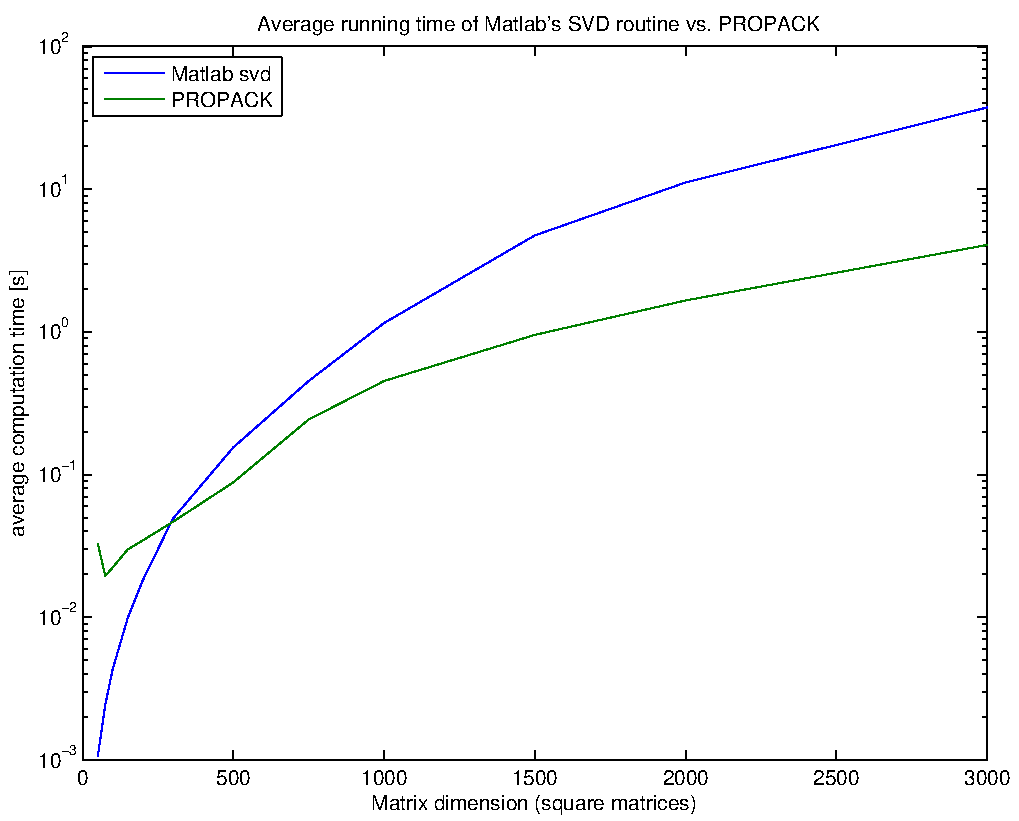
\includegraphics[width=0.75\textwidth]{../figures/svd_comparison}
\caption{Numerical comparison of Matlab's and PROPACK's SVD routines}
\label{Algorithms:Discussion:SVD:MatlabVSPropack:figure}
\end{figure}


When the matrix under consideration is sparse, the SVD can be carried out much faster using specialized methods~\cite{Berry:2005uq}. Unfortunately, while the iterates of the matrix~$S_k$ (in case of primal algorithms) are indeed sparse, the matrices for which the SVD actually needs to be computed are not. Therefore it does not seem clear how sparse SVD methods could help in improving performance of SVD-based Robust PCA algorithms. 


%%%%%%%%%%%%%%%
\subsubsection{Partial SVD methods}
\label{Algorithms:Discussion:SVD:PartialSVD:Subsubsec}

If we look at the a Singular Value Thresholding operation it is obvious that we really only needs to compute those singular values that lie above the specified threshold (which is known a priori in each step and does not depend on the singular values), since the other singular values will be set to zero anyway. One possibility to speed up the algorithms that involve thresholding of singular values is therefore to use a partial SVD to compute only those singular values of interest. For the APG algorithm the authors of~\cite{Lin:2010fk} use the software PROPACK that allows the computation of such a partial SVD. However, PROPACK by default requires the dimension of the principal singular space whose singular values are larger than the threshold, which is of course unknown a priori. Since it turns out that the rank of the the iterates~$L_k$ in the APG algorithm is monotonically increasing, a reasonable prediction of this dimension is not too hard~\cite{Lin:2010fk}. Doing so then allows to a partial SVD at each step rather than a full SVD, which can potentially speed up the algorithm (if the partial SVD can be computed efficiently). 

The PROPACK package has later also been modified to allow the computation of those singular values above a given threshold~\cite{Lin:2011kx}. Figure~\ref{Algorithms:Discussion:SVD:lasvdThrVSlasvd:figure} shows a comparison of the computation times of PROPACK's standard (full) SVD routine and the algorithm~\cite{Lin:2011kx} for different thresholds. Contrary to what one would expect, the full SVD in all cases is significantly faster than the partial SVD. At this point it is not clear what the reason for this is. Either the algorithm for performing the ``thresholded SVD'' itself is very slow, or the implementation that is provided by~\cite{Lin:2011kx} is very inefficient (or both). Either way, with the currently available implementation it does not seem to make sense to compute partial SVDs. 
%
\begin{figure}[htbp]
\centering
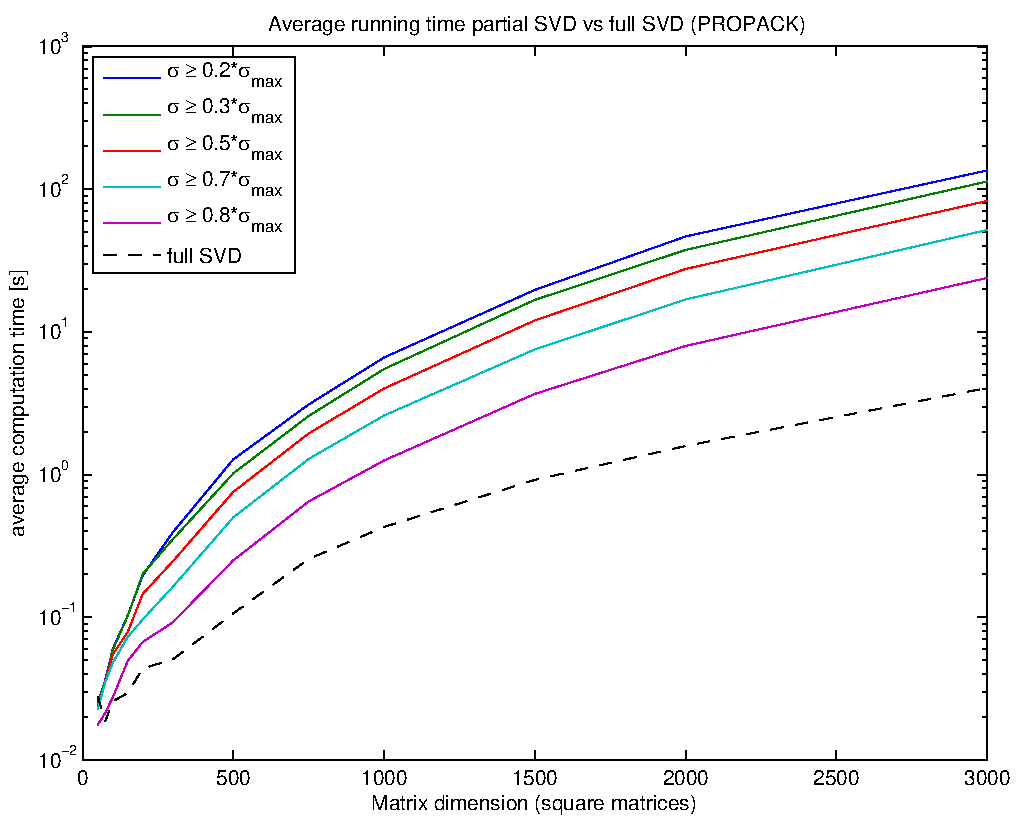
\includegraphics[width=0.75\textwidth]{../figures/thresh_svd_comparison}
\caption{Numerical comparison of partial and full SVD via PROPACK}
\label{Algorithms:Discussion:SVD:lasvdThrVSlasvd:figure}
\end{figure}





%
%
%This implementation can be used also in the ALM algorithms, where singular value thresholding is applied to matrices of the form $M-S_{k} +\mu_k^{-1}Y_{k}$.


%%%%%%%%%%%%%%%
\subsubsection{Warm-start methods for SVD}
\label{Algorithms:Discussion:SVD:WarmstartSVD:Subsubsec}


Another potential way of speeding up many SVD-based algorithms is to exploit the fact that the matrix of which the SVD has to be computed does generally not change much between iterations, in particular after a few iterations. To utilize this fact, the authors of~\cite{Lin:2010uq} propose a warm start technique for the block Lanczos method for SVD computation. 

Figure~\ref{Algorithms:Discussion:SVD:BLWScomptarison:figure} shows a comparison of the performance of the warm-start block Lanczos method~\cite{Lin:2010uq} on synthetic data of different size. It can be seen that the running time of the warm-start method is roughly two thirds of that of the standard method, over all dimensions considered in the simulation. The relative errors of the solution, given by $\|\hat{L}-L\|_F/\norm{L}{F}{}$ and $\|\hat{S}-S\|_F/\norm{S}{F}{}$, respectively, are generally worse than those of the standard method. This is due to the fact that only an approximate SVD is computed at each iteration. What is remarkable in Figure~\ref{Algorithms:Discussion:SVD:BLWScomptarison:figure} is that the number of iterations is essentially independent of the matrix size. Note however that this strong consistency very likely also has to do with the fact that all the considered randomly generated matrices are structurally identical. 

We want to emphasize here that the implementation of the warm-start block Lanczos method, as provided by~\cite{Lin:2011kx}, is completely Matlab-based and not fully optimized for performance. A careful implementation of the overall warm-start block Lanczos based inexact ALM algorithm in a performance-oriented language such as~C can be expected to yield further speedups. Nevertheless, even with the current implementation it is possible to solve rather large problems quite fast, with problems involving matrices with tens of million entries being solved in a few minutes. 

\begin{figure}[htbp]
\centering
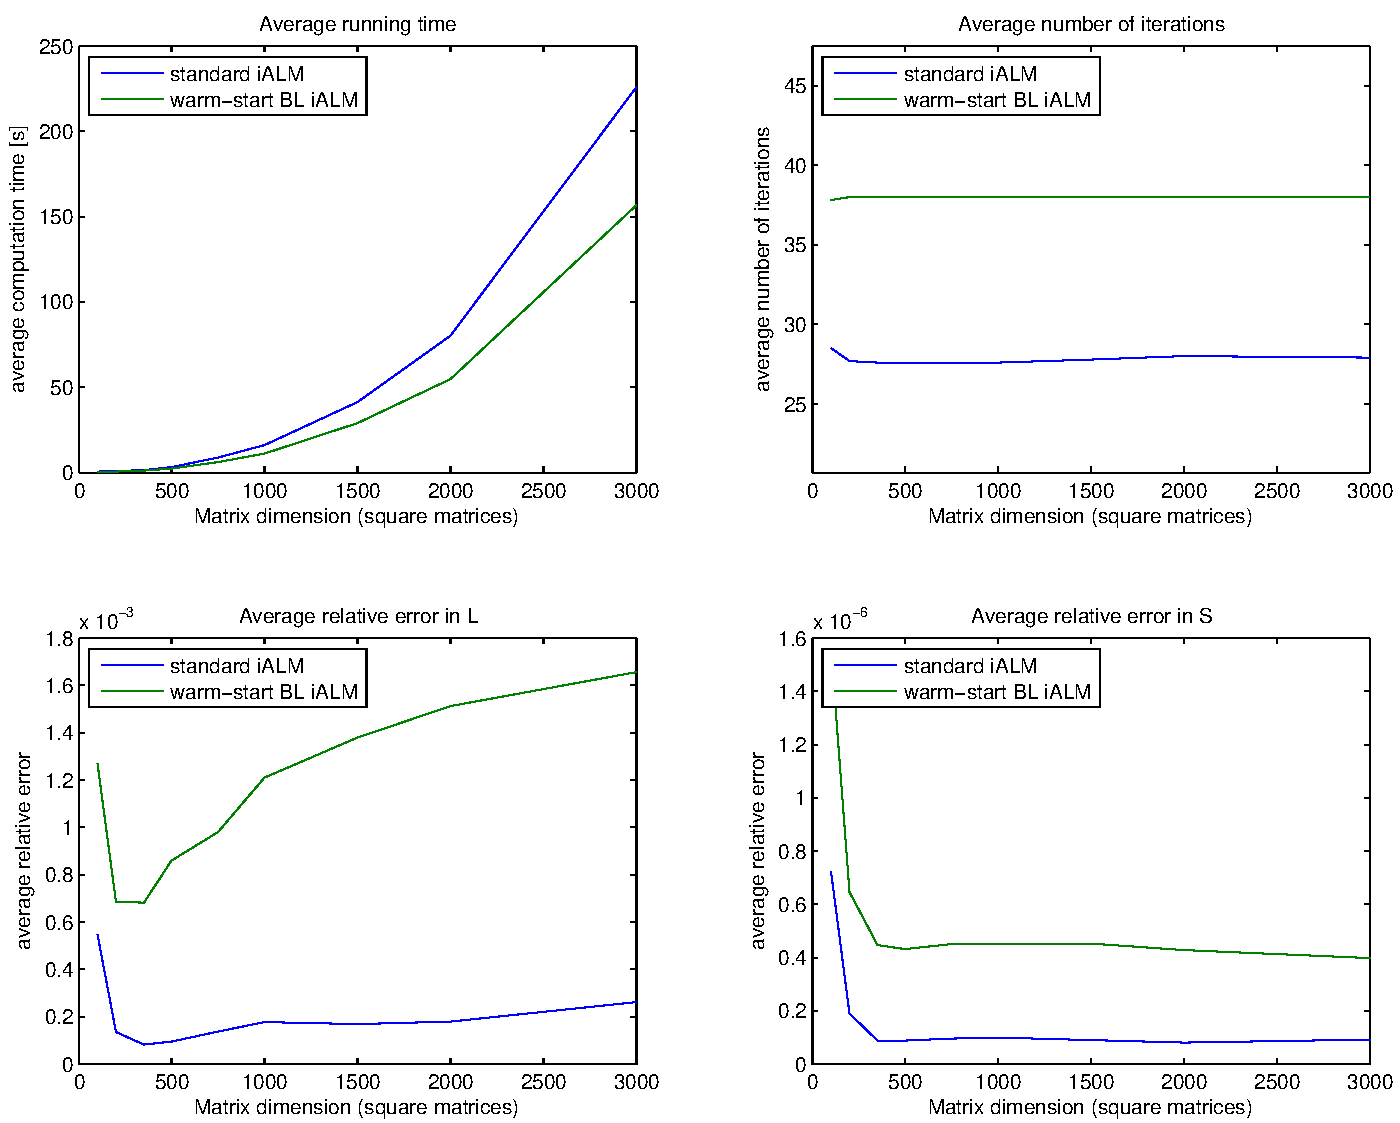
\includegraphics[width=0.95\textwidth]{../figures/BLWS_comparison}
\caption{Numerical comparison of warm-start vs. standard Block-Lanczcos method}
\label{Algorithms:Discussion:SVD:BLWScomptarison:figure}
\end{figure}







%%%%%%%%%%%%%%%%%%%%%%%%%%%%
\subsection{Possible Directions for Parallelization}
\label{Algorithms:Discussion:Parallel:Subsec}

With the advent of highly parallelized computing architectures in modern CPUs and GPUs, a number of projects have been devoted to the development and implementation of algorithms that exploit this massive computing power. Examples for these are MAGMA~\cite{Smith:2010tg} and CULA~\cite{Humphrey:2010kl}, which are adapting classic high-performance linear algebra packages such as LAPACK and BLAS to the highly parallelized architecture of modern GPUs. 

Some of the steps in the algorithms are inherently parallelizable, for example the entry-wise soft-thresholding of a matrix. Other steps require more work to be able to 

\cite{Boyd:2011hc}



%%%%%%%%%%%%%%%%%%%%%%%%%%%%%%%%%%%%%%%%%%%%
\section{Outlook: Algorithms for Stable Principal Component Pursuit}
\label{Algorithms:StablePCP:Sec}

As discussed in section REFERENCE, the results obtained for the Robust PCA problem have been extended to the case when in addition to the sparse noise, the data is corrupted also by a small non-sparse noise component~\cite{Zhou:2010vn}. This problem is usually referred to as Stable Principal Component Pursuit (Stable PCP). The associated optimization problem is 
%
\begin{align}
\begin{split}
p^* = \min_{L,S} \; &\norm{L}{*}{} + \lambda \norm{S}{1}{} \\
\text{s.t.} \quad &\norm{M - L - S}{F}{} \leq \delta
\end{split}
\label{Algorithms:StablePCP:StablePCP}
\end{align}
%
where $\delta>0$ is given. 

In~\cite{Aybat:2011vn} a number of different algorithms for Stable PCP are discussed, most of which are based on a smoothed or partially smoothed objective function and the application of Nesterov's optimal algorithms~\cite{Nesterov:2005fk}, which yields a theoretical complexity of~$O(1/\varepsilon)$. The authors also propose a first-order algorithm that works directly with the fully non-smooth objective. While they were not able to derive theoretical complexity results, empirical evidence suggests that this algorithm is very efficient in solving the problem. 





%%%%%%%%%%%%%%%%%%%%%%%%%%%%%%%%%%%%%%%%%%%%%%%%%%%%%%%%%%%%%%%%%%%%
\bibliographystyle{abbrv}
\bibliography{../../common/RobustPCA}


%%%%%%%%%%%%%%%%%%%%%%%%%%%%%%%%%%%%%%%%%%%%%%%%%%%%%%%%%%%%%%%%%%%%
\end{document}  






%============================================================================================
%============================================================================================
\chapter{Applications}
% !TEX root = ../report/report.tex

%%%%%%%%%%%%%%%%%%
% EE227A Project by Nathan Lam
%%%%%%%%%%%%%%%%%%


\section{Overview}

This section will review some applications using Robust PCA. Currently, most of the applications are related to computer vision. As we will show later, many images involve natural characteristic of low-rank structure, which makes Robust PCA a perfect fit to them. We will also explore some other applications that is theoretically with low-rank and sparse structure and show what we get from them. 

\section{Robust PCA Applications}

\subsection{Background modeling from surveillance video}

Video is a natural candidate for low-rank modeling, due to the correlation between frames. One of the most basic algorithmic tasks in video surveillance is to estimate a good model for the background variations in a scene. This task is complicated by the presence of foreground objects: in busy scenes, every frame may contain some anomaly. The background model needs to be flexible enough to accommodate changes in the scene, for example due to varying illumination In such situations, it is natural to model the background variations as approximately low rank. Foreground objects, such as cars or pedestrians, generally occupy only a fraction of the image pixels and hence can be treated as sparse errors.

\begin{figure}[h]
  \centering
  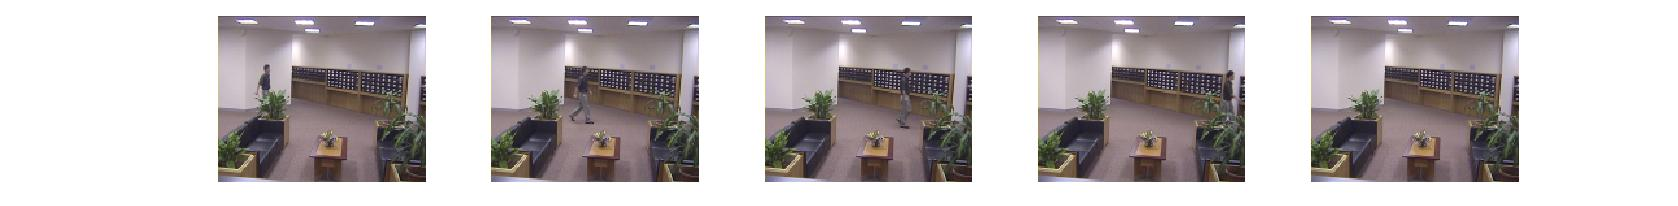
\includegraphics[width=1\textwidth]{../figures/SwitchLight_original.jpg}
  \caption{Original video frames}
  \label{fig:video:original}
\end{figure}

\begin{figure}[h]
  \centering
  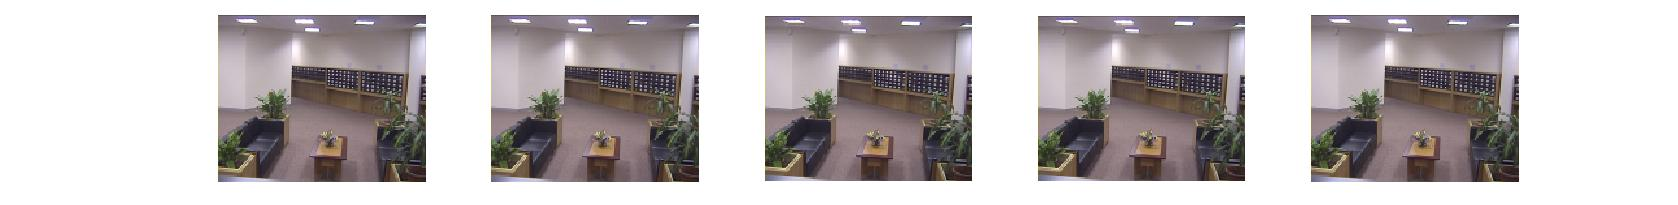
\includegraphics[width=1\textwidth]{../figures/SwitchLight_low_rank.jpg}
  \caption{Low-rank components}
  \label{fig:video:low_rank}
\end{figure}

\begin{figure}[h]
  \centering
  
\includegraphics[width=1\textwidth]{../figures/SwitchLight_sparse.jpg}
  \caption{Sparse components}
  \label{fig:video:sparse}
\end{figure}

We consider five frames from an original video, as shown in fig.~\ref{fig:video:original}, which is a scenario that  one man passes by. The resolution of each frame is $176\times144$. We first separate them into three channels (RGB). For each channel, we stack each frame as a column  of our matrix $M\in\mathbb{R}^{25344\times5}$. We decompose $M$ into low-rank components $L$ and sparse components $S$ by Robust PCA. Then we combine the three channels again to form images with low-rank component and sparse components respectively. We are using a 2GHz qual core laptop and it takes 0.92s to finish decomposition for three channels. We can find that the $L$, as shown in fig.~\ref{fig:video:low_rank}, correctly recovers the background, while $S$, as shown in fig.~\ref{fig:video:sparse}, correctly identifies the moving person.

The same setting is used into our own video that we took in UC Berkeley. The resolution in our video is $480\times640$, which is consistent with the resolution of most of the cell phone camera. Figure ~\ref{fig:video:campus:capture1} shows the result that we use 5 images which are taken every one second. It takes 15 seconds to finish. We can see that even though there are more than one person there, as long as the noise (here is the foreground) is sparse, the Robust PCA can still separate background and foreground. Since it does not consume too much time, this scenario can be considered as an application that removing wandering people when someone takes a picture.

\begin{figure}[h]
  \centering
  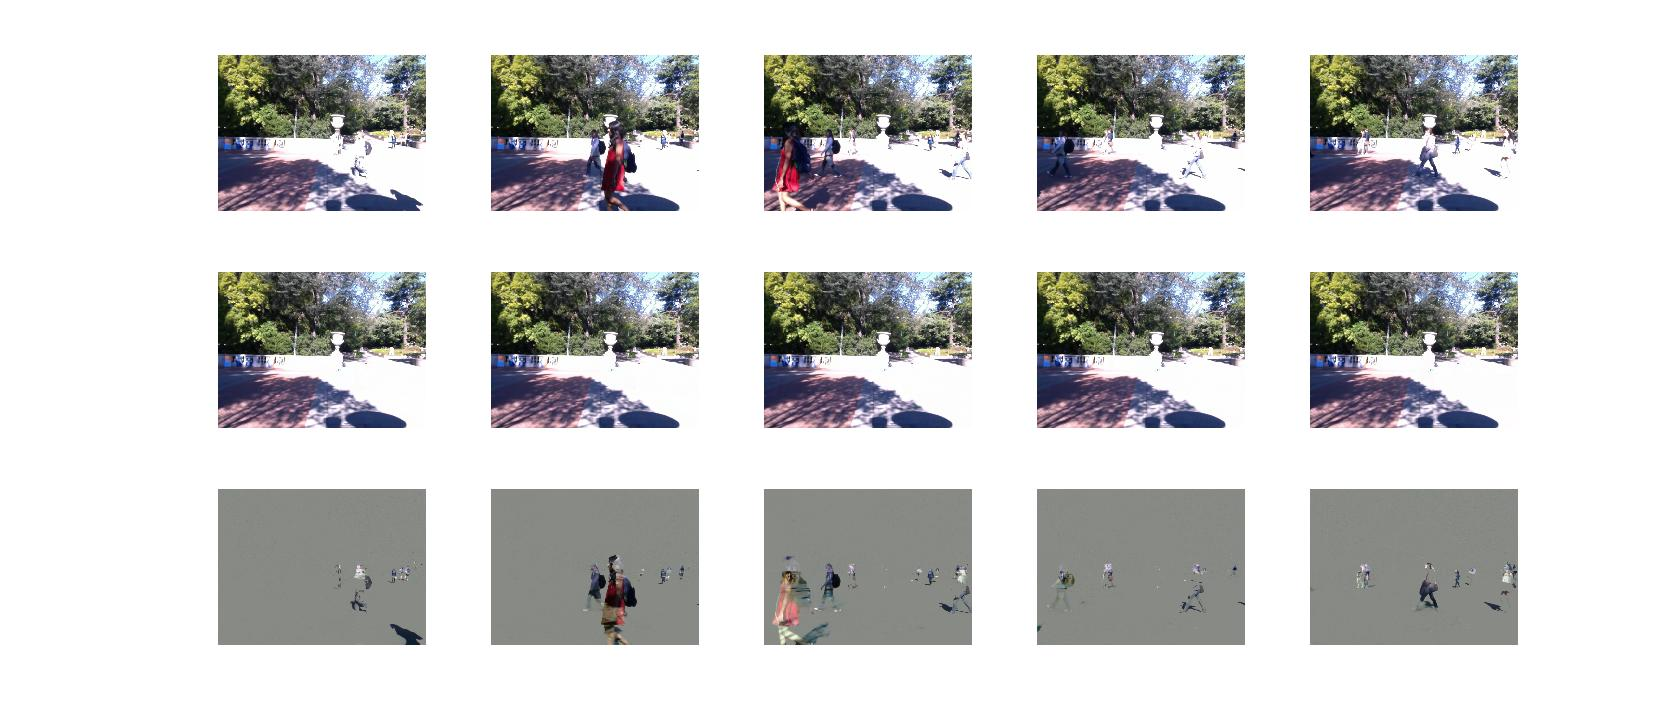
\includegraphics[width=1\textwidth]{../figures/campus_capture1.jpg}
  \caption{Perfect decomposition from campus video frames}
  \label{fig:video:campus:capture1}
\end{figure}

\begin{figure}[h]
  \centering
  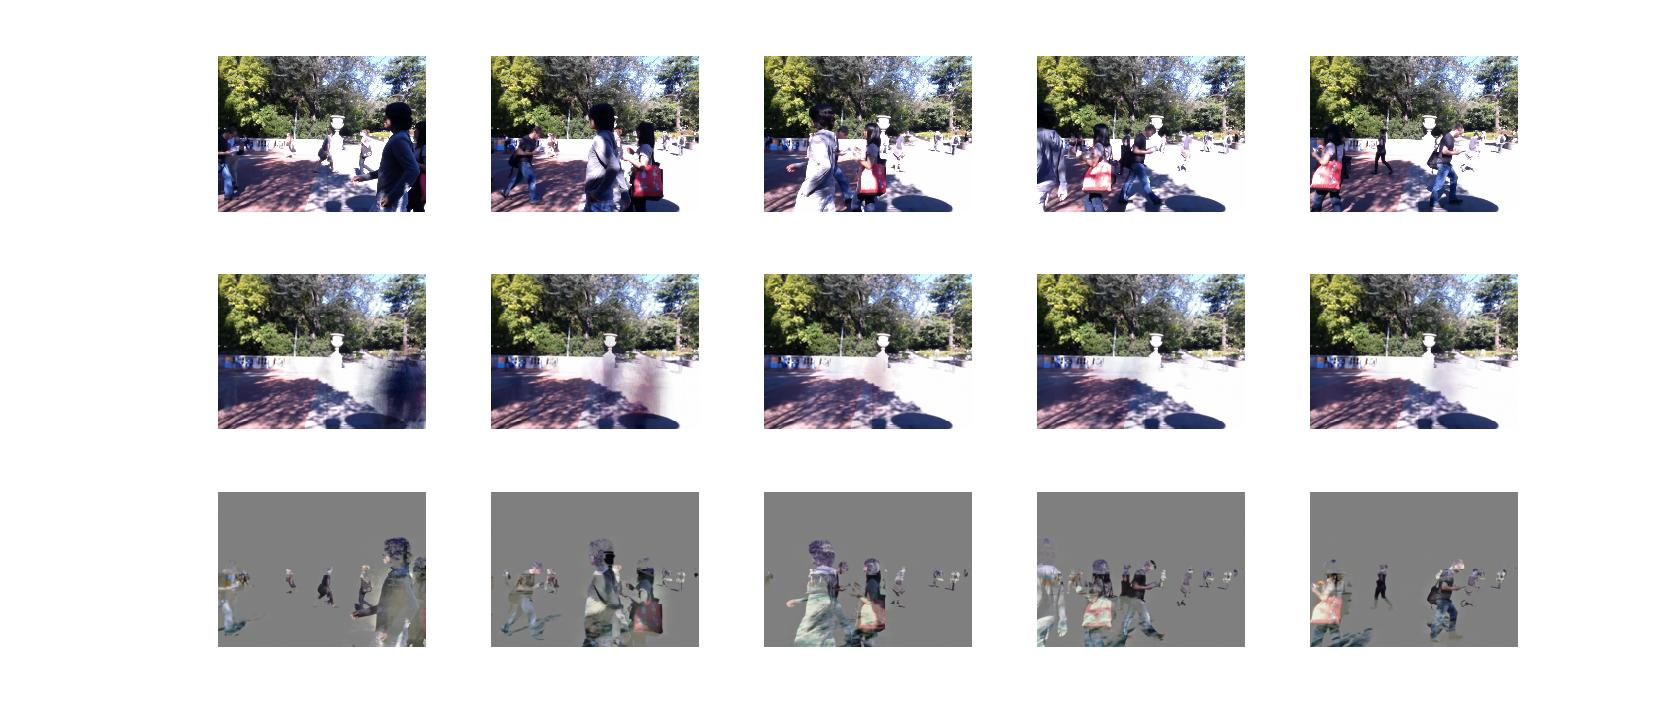
\includegraphics[width=1\textwidth]{../figures/campus_capture2.jpg}
  \caption{Imperfect decomposition from campus video frames}
  \label{fig:video:campus:capture2}
\end{figure}

Finally, we used all the frames from the 30 seconds video to run Robust PCA. We first down-sample them into $160\times214$ resolution in order to reduce the running time. We capture some frames from the resulting video. Most frames are good, but some are imperfect in terms of separating the foreground and background. We can find that in fig.~\ref{fig:video:campus:capture2}, when the foreground objects are dense, there are some "ghost" foreground people appearing in background video frames. To explain this result, we consider the following matrix:
\[
 M =
 \begin{bmatrix}
  100 & 100 & 100 & 100 & 100 \\
  100 & 100 & 100 & 100 & 100 \\
  0 & 0 & 100 & 100 & 100 \\
  100 & 100 & 100 & 100 & 100 \\
 \end{bmatrix}
\]
We can seperate $M$ into low-rank component and sparse component by Robust PCA. However, Robust PCA will favor a decomposition as:
\[
 M =
 \begin{bmatrix}
  100  & 100  & 100  & 100  & 100 \\
  100  & 100  & 100  & 100  & 100 \\
  0     &  0      & 100  & 100  & 100 \\
  100  & 100  & 100  & 100  & 100 \\
 \end{bmatrix}
 =
 \begin{bmatrix}
  100  & 100  & 100  & 100  & 100 \\
  100  & 100  & 100  & 100  & 100 \\
   34.0   & 34.0   & 36.8   & 36.8   & 36.8   \\
  100  & 100  & 100  & 100  & 100 \\
 \end{bmatrix}
 +
 \begin{bmatrix}
          0    &      0   &       0     &     0    &      0 \\
         0    &      0    &      0    &      0    &      0 \\
  -34.0  & -34.0   & 63.2   & 63.2   & 63.2 \\
         0    &      0   &       0     &     0     &     0 \\
 \end{bmatrix}
\]
such that $||L||_{*} + \lambda||S||_{1}  = 513.64$ 
rather than 
\[
 M =
 \begin{bmatrix}
  100  & 100  & 100  & 100  & 100 \\
  100  & 100  & 100  & 100  & 100 \\
  0     &  0      & 100  & 100  & 100 \\
  100  & 100  & 100  & 100  & 100 \\
 \end{bmatrix}
 =
 \begin{bmatrix}
  100  & 100  & 100  & 100  & 100 \\
  100  & 100  & 100  & 100  & 100 \\
  100  & 100  & 100  & 100  & 100 \\
  100  & 100  & 100  & 100  & 100 \\
 \end{bmatrix}
 +
 \begin{bmatrix}
          0    &      0   &       0     &     0    &      0 \\
         0    &      0    &      0    &      0    &      0 \\
  -100  & -100   & 0   & 0   & 0 \\
         0    &      0   &       0     &     0     &     0 \\
 \end{bmatrix}
\]
such that $||L||_{*} + \lambda||S||_{1}  = 536.66$ \\

From the above example, we can see that if most of the frames are corrupted in given pixels, Robust PCA hardly separates the background and foreground at those pixels perfectly. One way to solve it is to adjust the value of $\lambda$, but it is generally hard to choose a $\lambda$ that fits the entire video. Despite that, Robust PCA is still good for separating background and sparse foreground moving objects.


%%%%%%%
\subsection{Using Robust PCA in speech recognition}
Intuitively, a consistent sound would be of low-rank structure. If someone is speaking with background noise which is consistent, we would believe that we can separate a clearer speech (the sparse component) from background noise (low-rank component) via Robust PCA framework. If we get a clearer speech signal, the accuracy of speech recognition with current standard technique will increase. According to this thought, we did an experiment and try to see whether Robust PCA works in such case.

\begin{figure}[h]
  \centering
  \subfloat[clean]{\label{fig:speech:clean}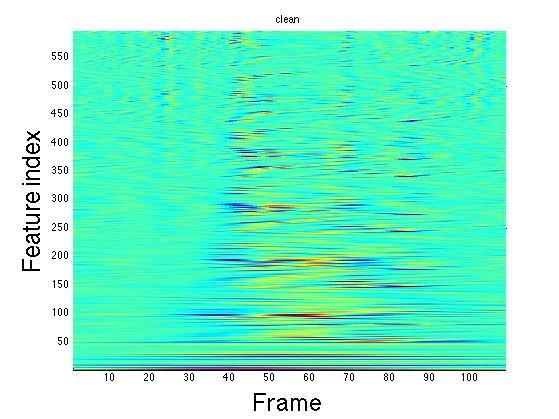
\includegraphics[width=0.5\textwidth]{../figures/speech_clean.jpg}}
  ~ %add desired spacing between images, e. g. ~, \quad, \qquad etc. (or a blank line to force the subfig onto a new line)
  \subfloat[noisy]{\label{fig:speech:noisy}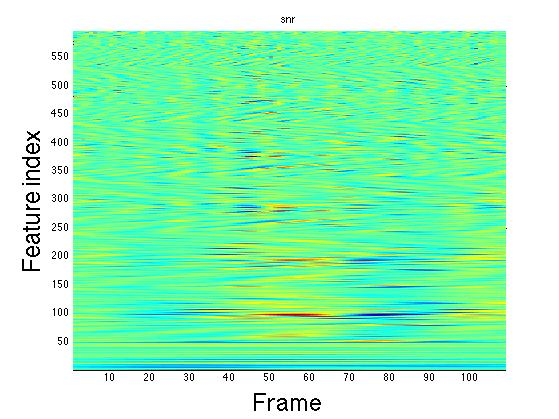
\includegraphics[width=0.5\textwidth]{../figures/speech_noisy.jpg}}
  ~ 
  \\ \subfloat[sparse]{\label{fig:speech:sparse}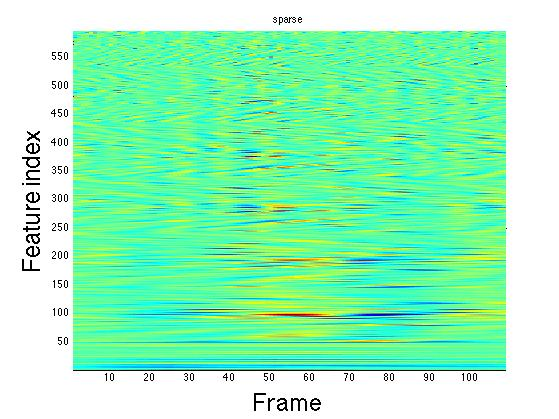
\includegraphics[width=0.5\textwidth]{../figures/speech_sparse.jpg}}
  ~
  \subfloat[low-rank]{\label{fig:speech:low_rank}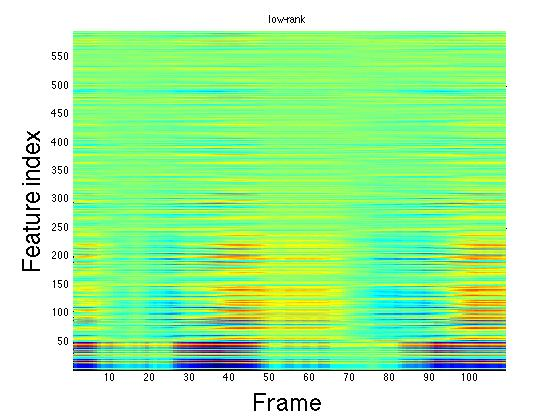
\includegraphics[width=0.5\textwidth]{../figures/speech_low_rank.jpg}}

  \caption{Speech features}
  \label{fig:speech}
\end{figure}

Figure~\ref{fig:speech:clean} shows the features of a clean speech signal, where the x-axis denotes indices of small time frames and the y-axis denote the features vectors at each frame. These features are computed by a standard method refering to \cite{}. Figure~\ref{fig:speech:noisy} shows the features domain of the same speech signal subjecting to noise with $SNR = 0$ in this case. We apply Robust PCA to decouple these features into low-rank component, as shown in fig.~\ref{fig:speech:low_rank}, and sparse component, as shown in fig.~\ref{fig:speech:sparse}. Technically, we would believe that sparse component is corresponding to our speech signal whereas low-rank component is corresponding to noise. Then we use the sparse component as new features and train a classifier via method in \cite{}. Unfortunately, comparing to the original method without  Robust PCA, we only got improvement in data set with subway noise, which we consider as the most consistent noise among the data set. In this data set, Robust PCA improve the accuracy rate with 3\% comparing to original method. For other noise, such as street noise and car noise, we both got decrease about 7\% in accuracy. One possible reason is that in the real world, most of the noise is not low-rank and they are not consistent. However, speech signal could be low-rank sometimes because there are only a limited vowels and consonants in a language, which makes Robust PCA not so suitable for de-noising.  

%%%%%%
%%%%%%
\subsection{Senators voting data analysis}
We have used Robust PCA to analyze voting data of the US senators. The data involves 100 senators voting at 542 bills around 2005 to 2008. The original data matrix is a $542\times100$ matrix with elements \{-1, 0, 1\}, representing voting for, against the bill and abstention. We first form a $100\times100$ covariant matrix and then run Robust PCA to this covariant matrix. We choose $\lambda = 1/\sqrt{10}$ as general. The rank of the low-rank component is 58 and the number of non-zero entries in sparse component is 6222. The results is shown in the following fig.~\ref{fig:vote:covariant}:


\begin{figure}[h]
  \centering
  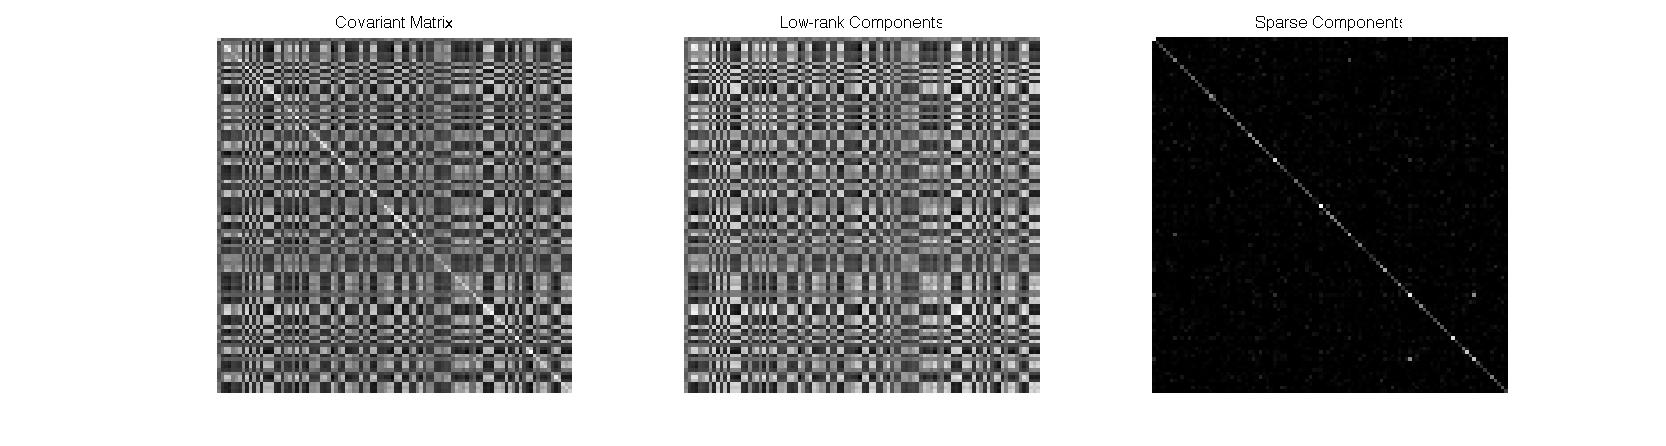
\includegraphics[width=1\textwidth]{../figures/vote_cov.jpg}
  \caption{Covariant matrix and its low-rank component and sparse component}
  \label{fig:vote:covariant}
\end{figure}

By analyzing the sparse component, we found that the sparse matrix seems to tell us some elements (i.e. senators) with strong connection. In general, the values in diagonal terms are large in sparse component because they are highly correlated. On the other hand, we could find there are some other highly correlated elements expect for the diagonal terms from the sparse matrix. We filter the value which is bigger than 0.8 in the sparse matrix expect for the diagonal terms. We found the following senators who are highly correlated in the sparse matrix: 1. (Specter, Snowe); 2. (Specter, Collins); 3. (Snowe, Collins) 4. (Jeffords, Collins) 5. (Dorgan, Conrad) 6. (Inouye, Akaka) 7. (McCain, Kyl). Interestingly, the real facts seem to match these results. First, the three Republican senators Specter, Snowe and Collins, who appear in pairs 1, 2 and 3, are always doing the same decisions, which can be shown by several reports\footnote{"The Gang of Three: Specter, Collins and Snowe" \url{http://usconservatives.about.com/b/2009/02/11/the-gang-of-three-specter-collins-and-snowe.htm}} \footnote{"NYT: Obama thanked Collins, Snowe, Specter for their �patriotism� \url{http://hotair.com/archives/2009/02/07/nyt-obama-thanked-collins-snowe-specter-for-their-patriotism/}}. Dorgan and Conrad in pair 5 are both from North Dakota. Inouye and Akaka in pair 6 are both from Hawaii. McCain and Kyl are both from Arizona. 

As shown is fig.~\ref{fig:vote:covariant:pca} and fig.~\ref{fig:vote:covariant:lr:pca}, we also compared the first two principal components in the original covariant matrix and the low-rank component. Their patterns remain similar with each other.  

\begin{figure}[h]
  \centering
  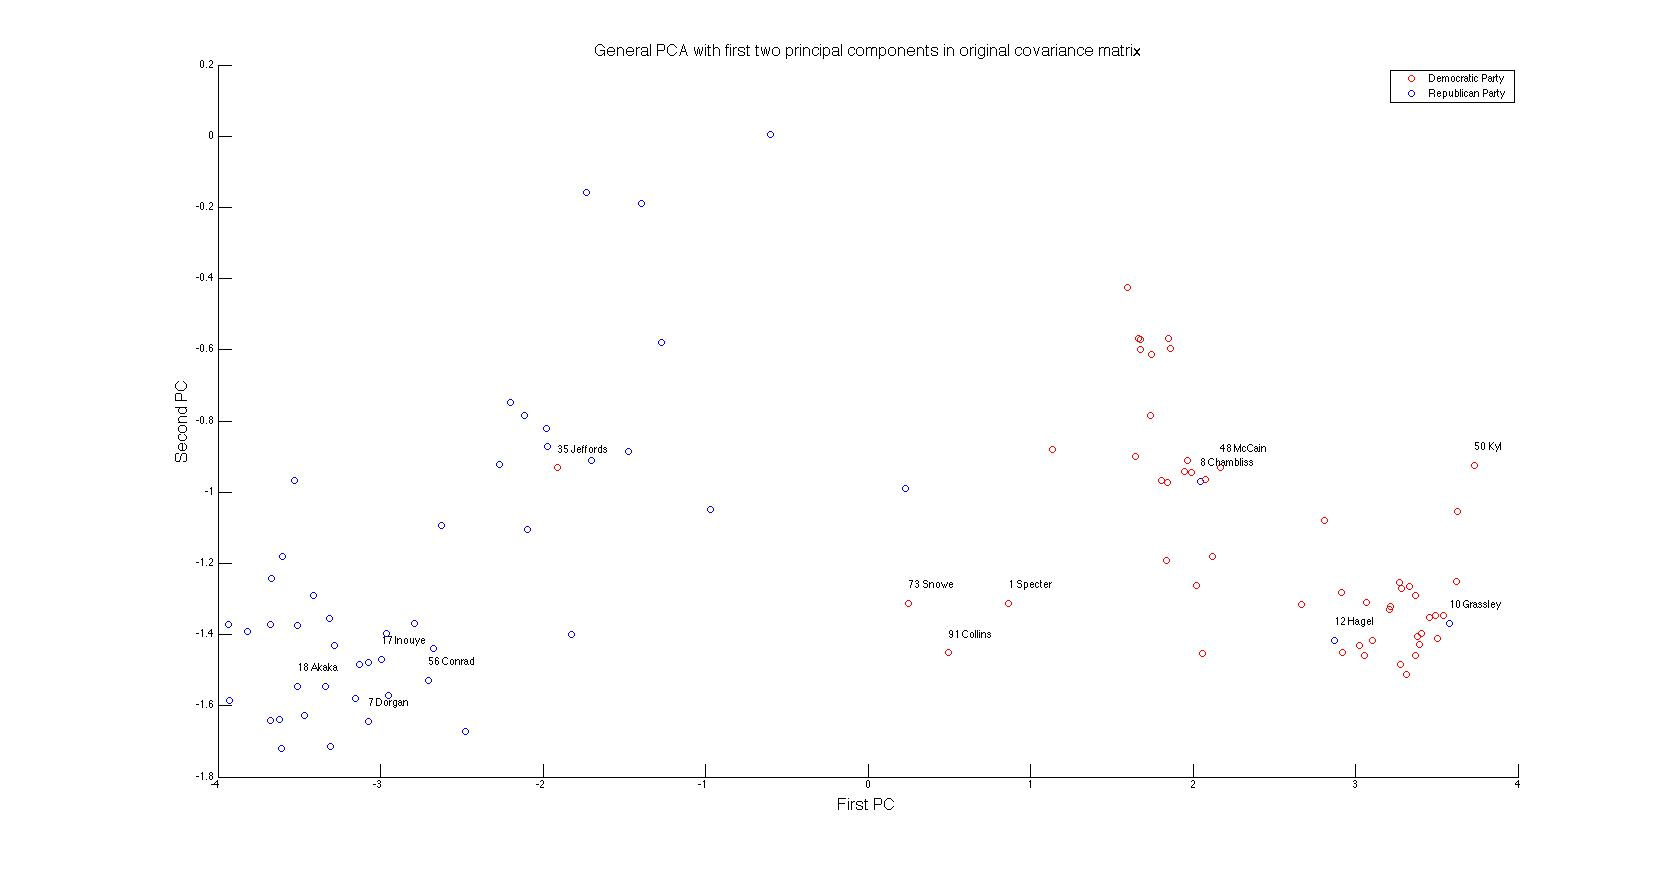
\includegraphics[width=0.85\textwidth]{../figures/vote_cov_mat_pca.jpg}
  \caption{General PCA with first two principal components in original covariant matrix}
  \label{fig:vote:covariant:pca}
\end{figure}

\begin{figure}[h]
  \centering
  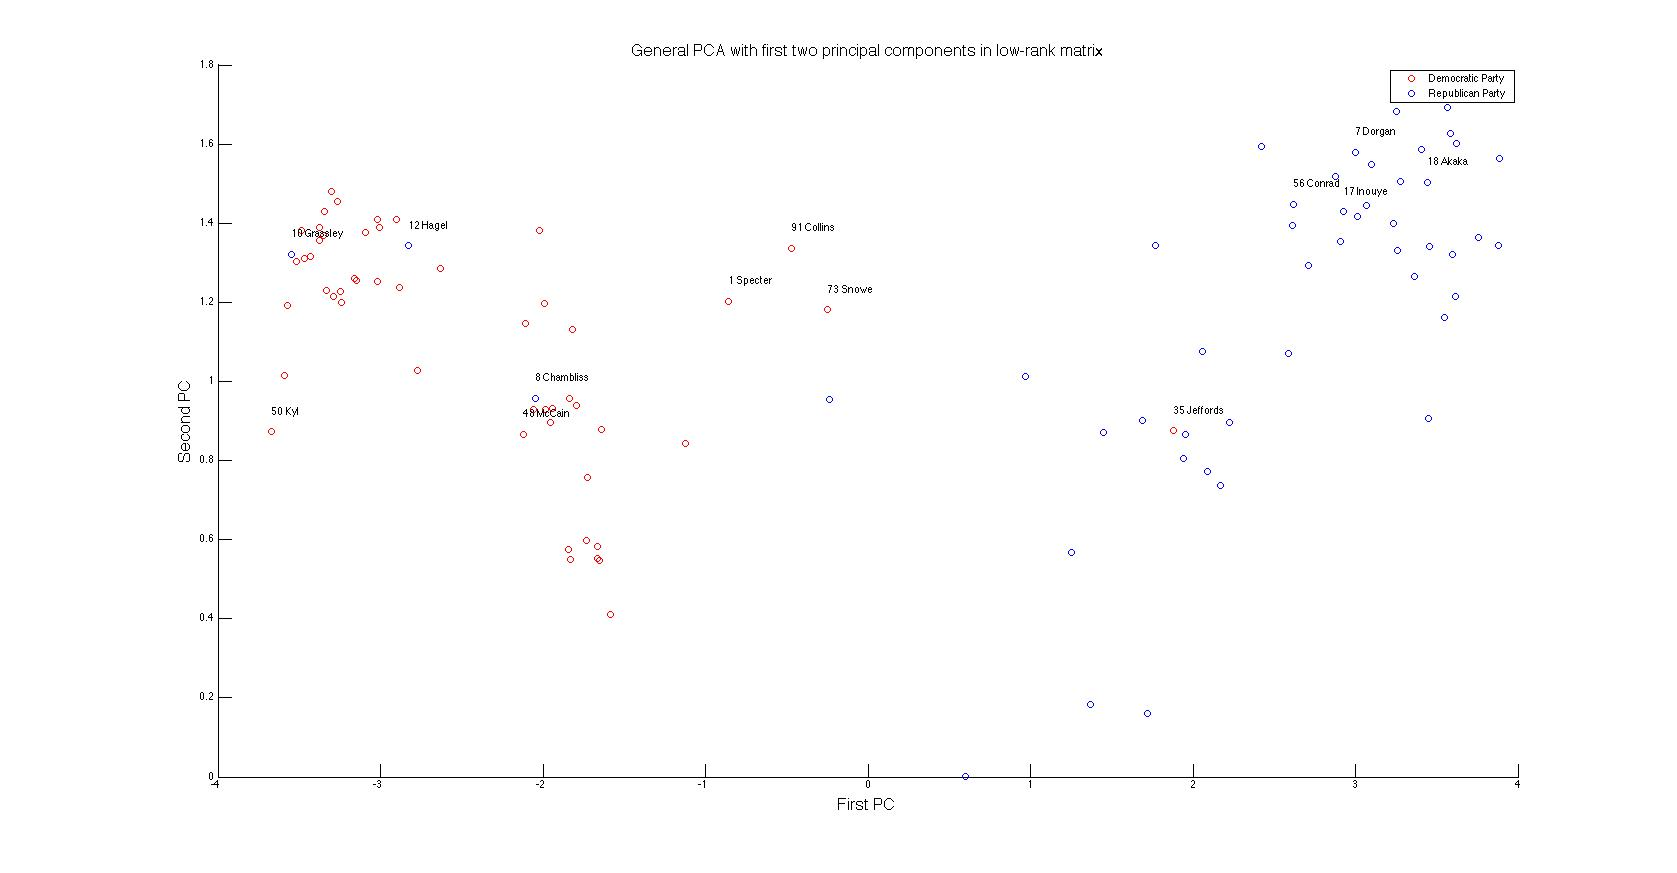
\includegraphics[width=0.85\textwidth]{../figures/vote_cov_lr_pca.jpg}
  \caption{General PCA with first two principal components in low-rank component of covariant matrix}
  \label{fig:vote:covariant:lr:pca}
\end{figure}



%%%%%
\subsection{Pre-processing of Brain-Machine Interface neural spike data}

We have used Robust PCA on some neural spike data that was collected from a monkey's brain. The Brain-Machine Interface project investigates how neural spike data can be used to interface with machines, with the ultimate goal of establishing some sort of bi-directional link (that is, to be able to control a machine through brain activity and, conversely, to ``feel'' feedback from measurements obtained by the machine). 

The particular problem we have looked at in this project was to use Robust PCA to analyze the neural spike data obtained from the motor cortex of a monkey, who was moving his arms to control a computer cursor in different directions. The assumption was that the measurements would consist of a somewhat ``low-rank'' component associated to the movement required by the particular task, and some superimposed sparse noise associated to neuron firings in the background. The data available was time-series neural spike data from a particular experiment, where the monkey had to move the cursor in 8 different directions, according to 45 degree increments. Each of the task was repeated a certain number of times. A total of 127 parallel measurement channels were available, each corresponding to a neuron (or a small number of neurons). 

As a pre-processing step, we normalized the time over the different trials for each component. The reasoning here was that the same task will correspond to the same neural firing pattern, independent of whether it was performed faster or slower\footnote{very little is known at this point about the structure of the dataset, so it was up to us to make reasonable assumptions about the data}. The next step was to group each of the trials for each of the tasks into a number of time bins, i.e. if the number of bins is~$N$ then the $i$-th bin associated to neuron~$k$ counts the number of firings of neuron~$k$ within the interval~$[(i-1)/N, i/N]$ (recall that trial time is normalized to~$1$). 

Figure~\ref{Applications:RPCAapps:BMI:raw3bins} shows the raw data after binning with 3 bins. 
%
\begin{figure}[h]
\centering
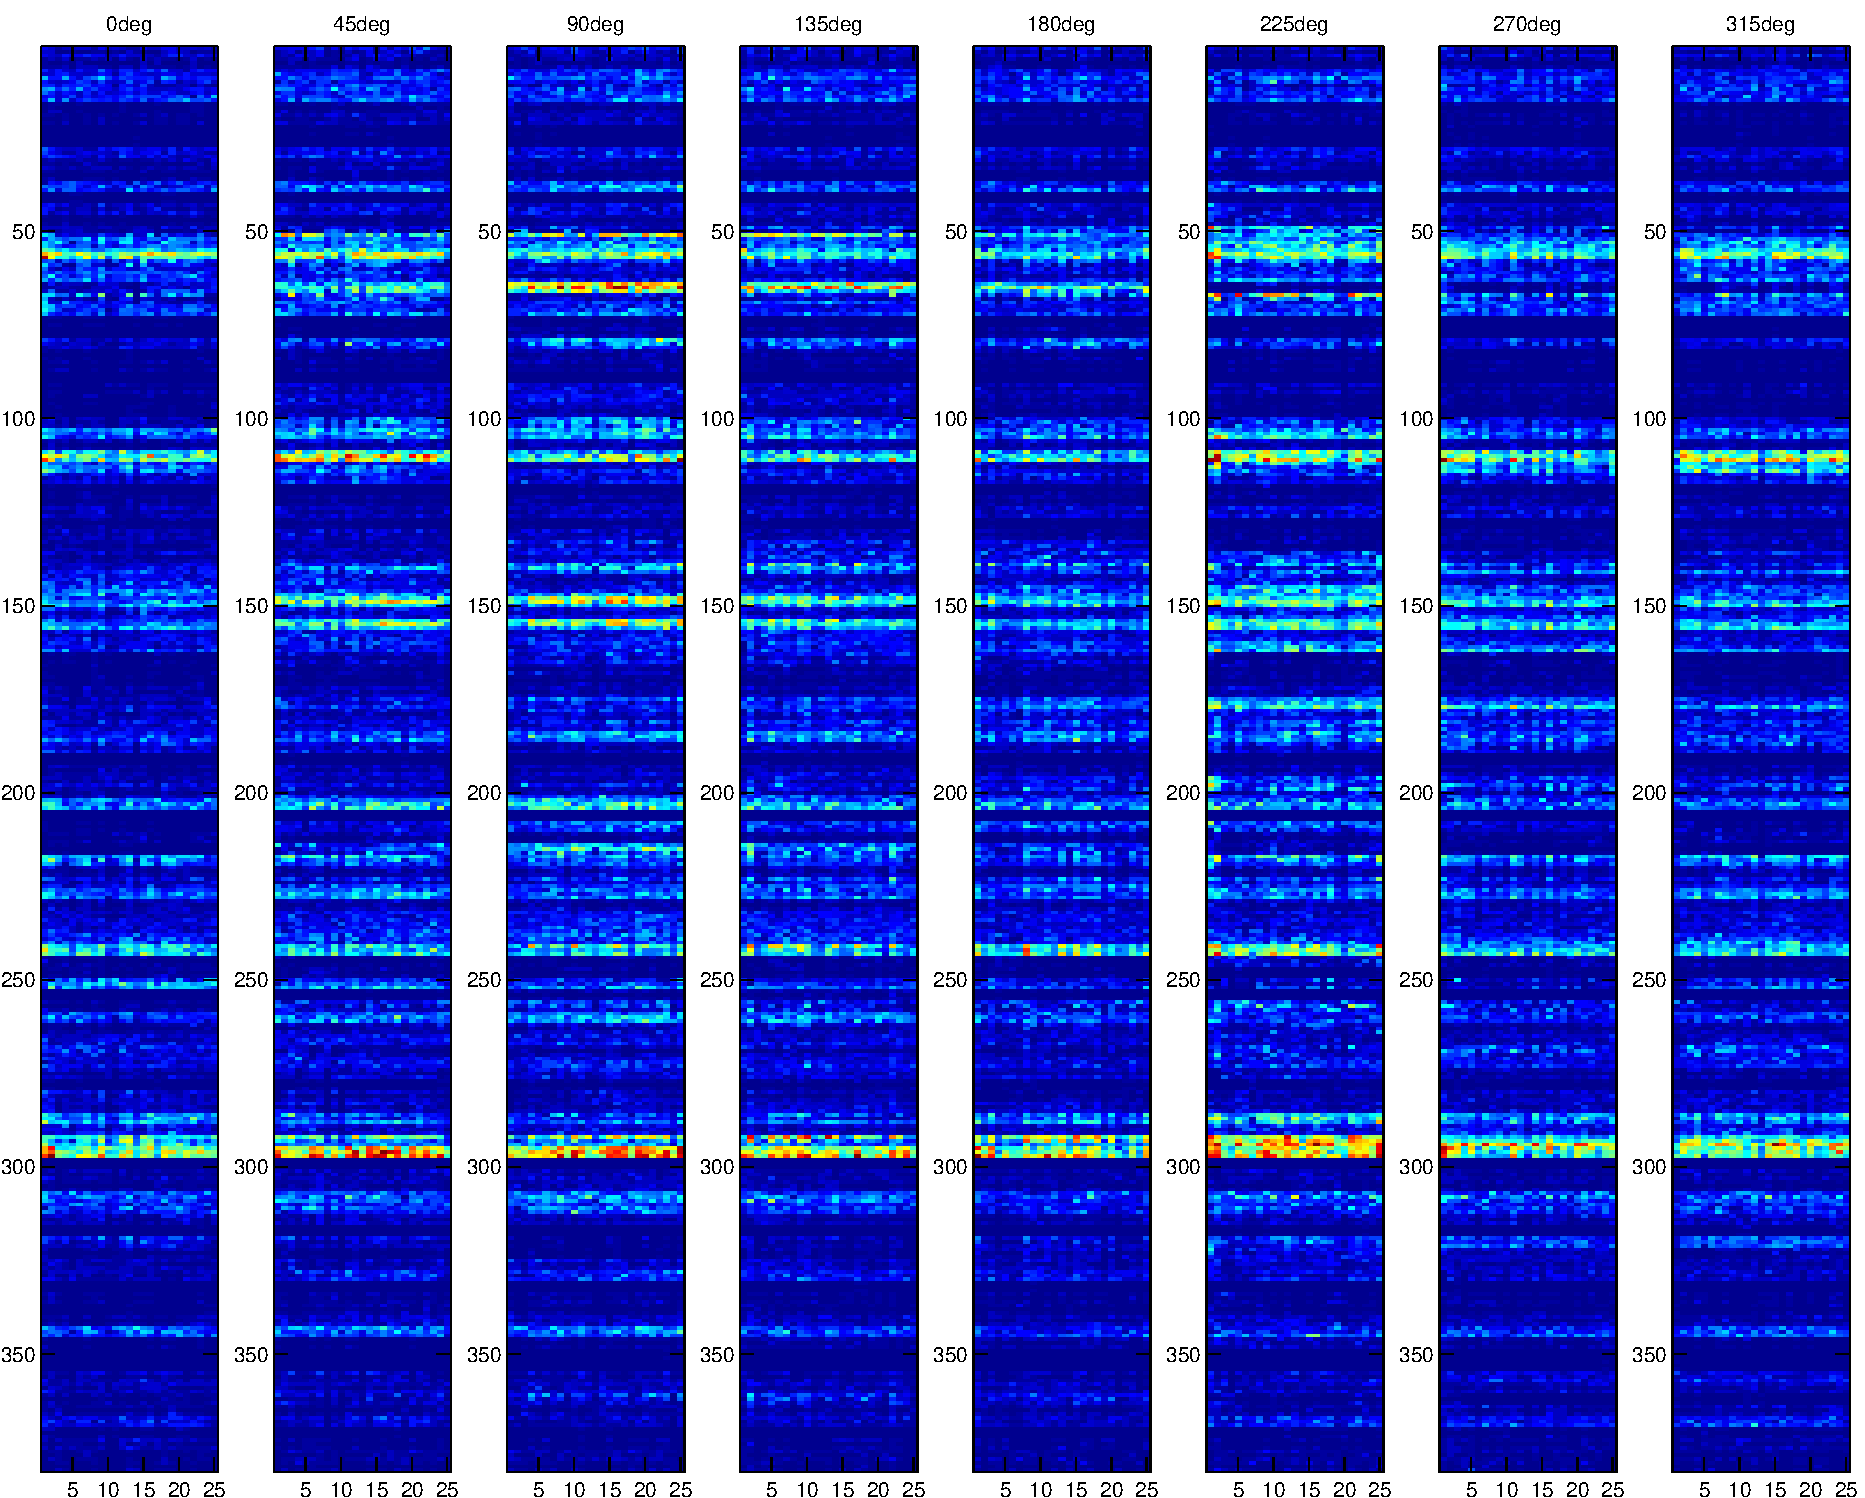
\includegraphics[width=\textwidth]{../figures/BMI_raw_3bins}
\caption{Raw (normalized and binned) neural spike data, $n_{bin}=3$}
\label{Applications:RPCAapps:BMI:raw3bins}
\end{figure}
%
here each of the 25 columns in each task represent the binned data from a single trial, where the 3 bins are stacked vertically. That is, within the large column associated to the $0\deg$ task, the first three entries of the first column correspond to the three time bins of the first neuron. The data is for 127 neurons, hence the overall matrix has $3\cdot127= 381$ rows. From the raw data in Figure~\ref{Applications:RPCAapps:BMI:raw3bins} we can already see some interesting features in the data, namely that each of the tasks seems to have its characteristic pattern. 

For each of the tasks we apply Robust PCA to the data matrix to extract low-rank and sparse components. Figure~\ref{Applications:RPCAapps:BMI:processed3bins} shows the low rank component extracted from the raw data of Figure~\ref{Applications:RPCAapps:BMI:raw3bins}. We notice that, as expected, the result is a ``filtered'' version of the raw data, in which the principal characteristics are retained while a sparse component has been removed. We think that the low-rank component in each of the tasks corresponds to the neuron firing pattern that can be directly related to the task, while the sparse component may be mis-detections, firings due to other movements, or simply sparse ``background'' firing that is always present.

%
\begin{figure}[h]
\centering
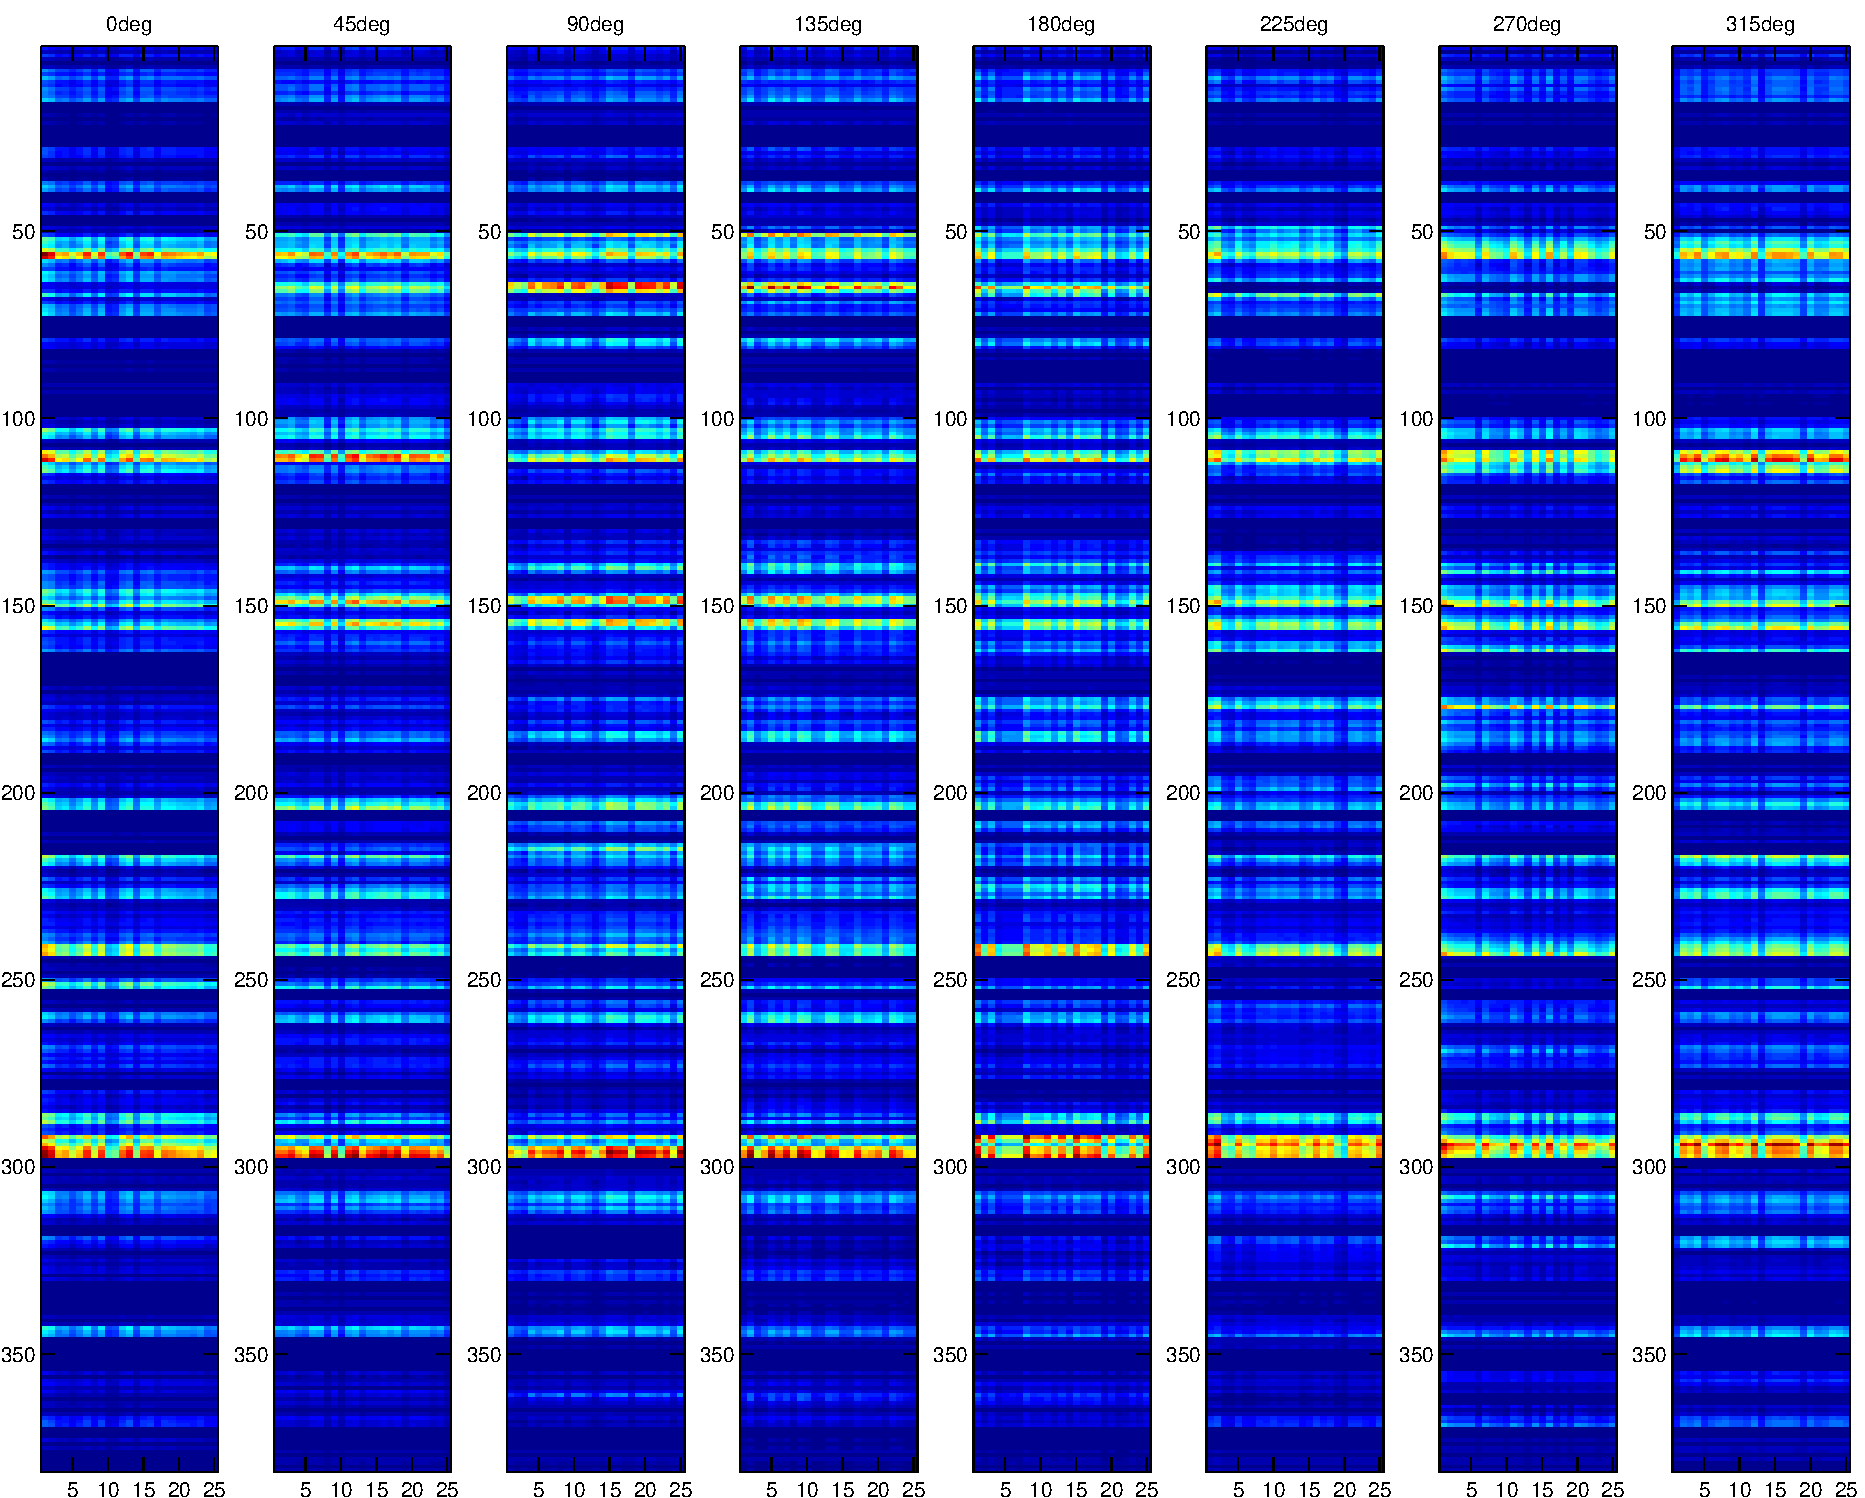
\includegraphics[width=\textwidth]{../figures/BMI_processed_3bins}
\caption{Processed neural spike data, $n_{bin}=3$}
\label{Applications:RPCAapps:BMI:processed3bins}
\end{figure}
%
For the $90\deg$ task Figure~\ref{Applications:RPCAapps:BMI:comparison90deg} shows a direct comparison of the raw data and the low-rank and sparse components obtained via Robust PCA. While for this comparably small data set the basic characteristics can be extracted visually just by looking at the matrix, this in general is not possible for high-dimensional data. One issue that we see with the available dataset is that the low rank component itself is quite sparse (since we are considering time-series data), hence some technical assumptions such as the incoherence condition will not necessarily hold. However, since not even neuroscientists have a clear understanding of what the data characteristics are and what the different patterns mean, we will not attempt to resolve this issue here. After the end of the semester we plan to learn more about the Brain-Machine interface project and, together with domain experts, to identify possible problems where Robust PCA could be used.

\begin{figure}[h]
\centering
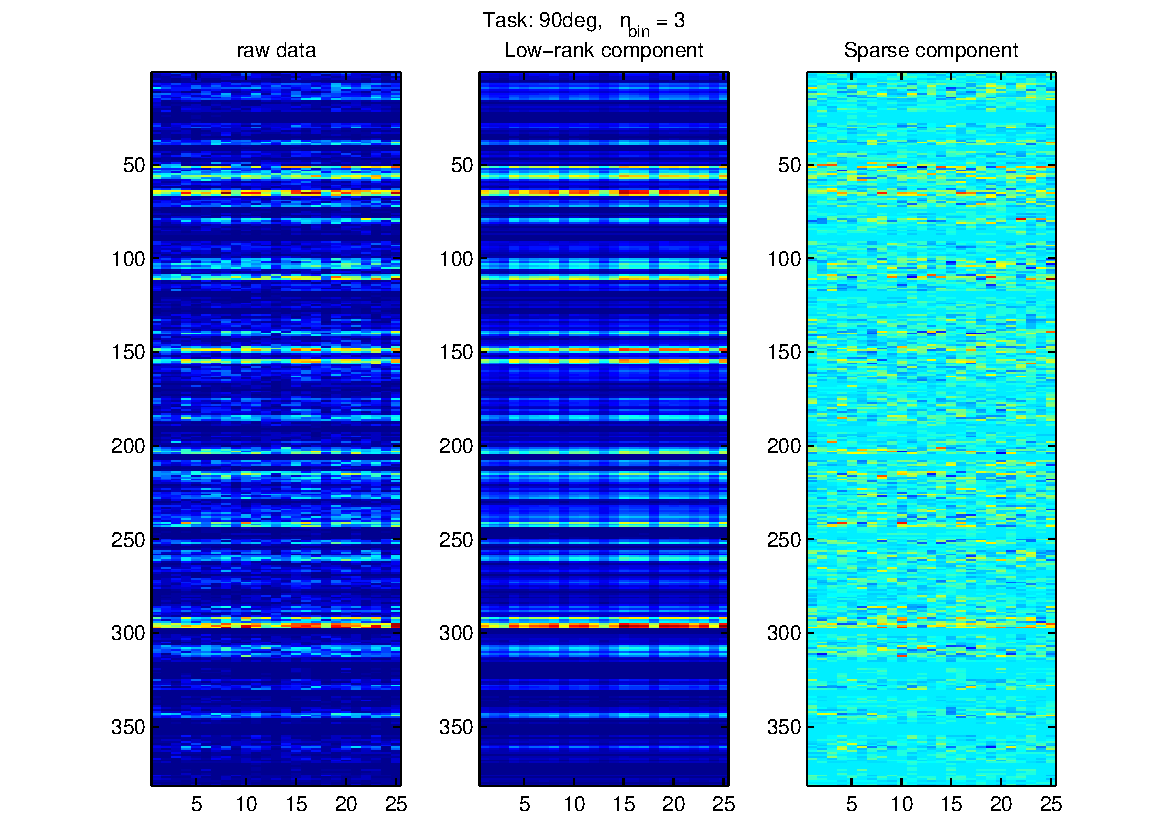
\includegraphics[width=0.95\textwidth]{../figures/BMI_comparison_90deg_3bins}
\caption{Raw data, low-rank component~$L$ and sparse component~$L$ for $90\deg$ task, $n_{bin}=3$}
\label{Applications:RPCAapps:BMI:comparison90deg}
\end{figure}

Based on the difference in neurons firing patterns between different tasks one can use machine learning techniques to predict from neural measurements which task the monkey is performing. Here Robust PCA could be used as a pre-processing step to filter out the sparse noise component. However, due to our lack of domain knowledge it is at this point unclear whether the Robust PCA framework has advantages over other and possibly simpler methods, for example a simple low-pass filters along the rows of the data matrix. Our main reason for presenting this application example here was to illustrate that Robust PCA can indeed be used as a tool to analyze interesting real data of reasonable size. 







\section{Discussion}
Robust PCA framework is a powerful tool to separate low-rank components and sparse components if we are given a combination of these two structures. However, generally most of the real world data is not directly a combination of these two structures unless the data is subjected to some kinds of transformation. One example is the data set of human faces with different expressions and illuminations. In this case, some researches have proposed some methods, RASL~\cite{Peng:2010} and TILT~\cite{Zhang:2011}, based on the original convex optimization problem in Robust PCA. They introduce transformation parameters to the original framework and by linearizing with respect to the transformation parameters, we got a new but not difficult convex problem. As long as the data is within a certain degree of transformation, the algorithms can still recover the low-rank structure and sparse structure.

We can also observe that is image data, the sparse noise is always presented as blocks. For example, the person in fig.~\ref{fig:video:sparse} appears in connected pixels, so the noise is not distributed randomly in pixels. A possible direction that can improve the separation in image data is that we can introduce a penalty term in the original optimization problem:
\begin{align}
\begin{split}
p^* = \min_{L,S} \; &||L||_{*} + \lambda \||S||_{1} + \beta\sum_{i, j\in\mathcal{N}(i)}^{} (S_{i} - S_{j})^2\\
\text{s.t.} \quad &M = L+S
\end{split}
\label{applications:discussion}
\end{align}
where $\mathcal{N}(i)$ means all the entries next to $i$ in matrix $S$. This problem is still convex so we can solve it via existing algorithm for convex optimization problems.








%============================================================================================
\newpage
\bibliographystyle{abbrv}
\bibliography{../../common/RobustPCA}

\end{document} 